\chapter*{Appendix}

\section{Chapter \ref{chap:routing}}


%figure : 3 time series (3 reservoirs) on average over the IP for both routings
\begin{figure}[htbp]
    \centering
    \begin{subfigure}[b]{0.48\textwidth}
        \caption{Groundwater reservoir average}
        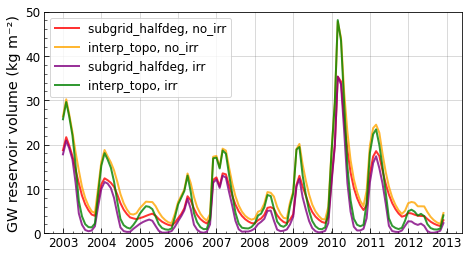
\includegraphics[width=\textwidth]{images/chap3/time_series/slowr_time_series.png}
    \end{subfigure}
        \begin{subfigure}[b]{0.48\textwidth}
        \caption{Groundwater reservoir average seasonal cycle}
        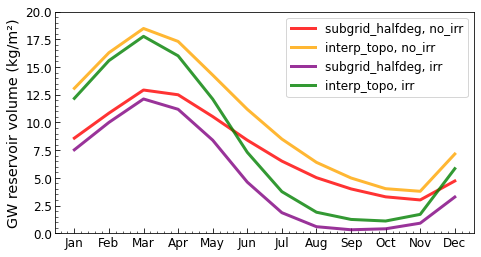
\includegraphics[width=\textwidth]{images/chap3/time_series/slowr_seasonal_cycle.png}
    \end{subfigure} \\
    
    \begin{subfigure}[b]{0.48\textwidth}
        \caption{Overland reservoir average}
        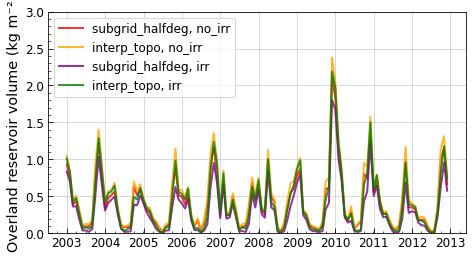
\includegraphics[width=\textwidth]{images/chap3/time_series/fastr_time_series.png}
    \end{subfigure}
    \begin{subfigure}[b]{0.48\textwidth}
        \caption{Overland reservoir average seasonal cycle}
        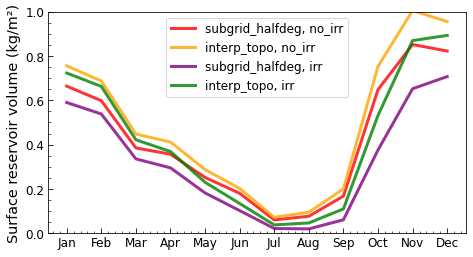
\includegraphics[width=\textwidth]{images/chap3/time_series/fastr_seasonal_cycle.png}
    \end{subfigure} \\
    
    \begin{subfigure}[b]{0.48\textwidth}
        \caption{River reservoir average}
        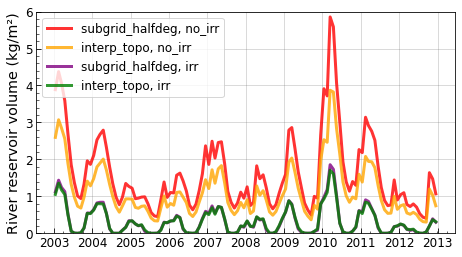
\includegraphics[width=\textwidth]{images/chap3/time_series/streamr_time_series.png}
    \end{subfigure} 
    \begin{subfigure}[b]{0.48\textwidth}
        \caption{River reservoir average seasonal cycle}
        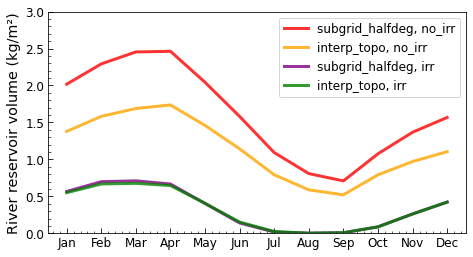
\includegraphics[width=\textwidth]{images/chap3/time_series/streamr_seasonal_cycle.png}
    \end{subfigure} \\

    \caption{Time series and seasonal cycles of reservoir volumes on average over the Iberian Peninsula domain.}
    \label{fig:reservoir_time_series}
\end{figure}

\section{Chapter \ref{chap:forcing}}
%Forcing influence

%figure : maps of relative diff vs ERA for 3 domain sizes
%todo:captions
\begin{figure}[htbp]
    \centering
    \begin{tabular}{ccc}
        %precip
        \begin{subfigure}[b]{0.33\textwidth}
            \caption{}
            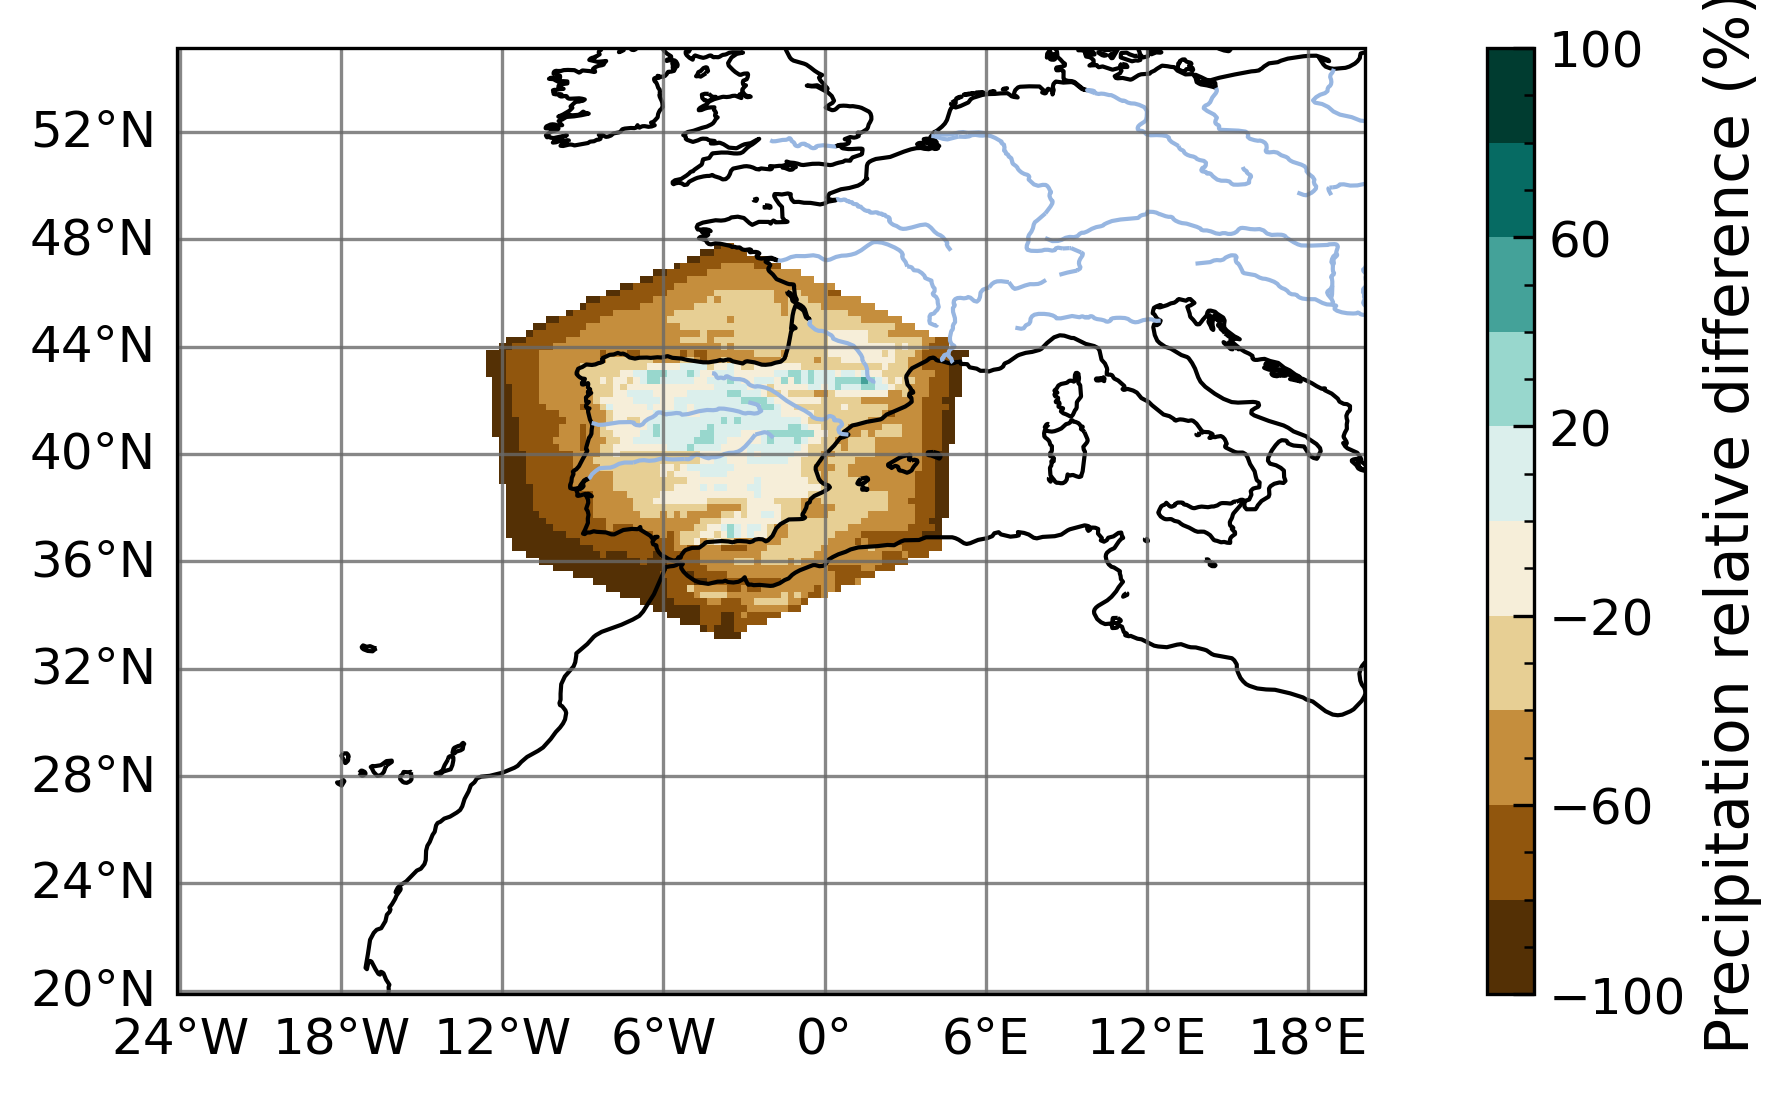
\includegraphics[width=\textwidth]{images/chap4/domain_size/rel_diff_map_precip_era_LAM_1000km_NBP40.png}
        \end{subfigure} &
        \begin{subfigure}[b]{0.33\textwidth}
            \caption{}
            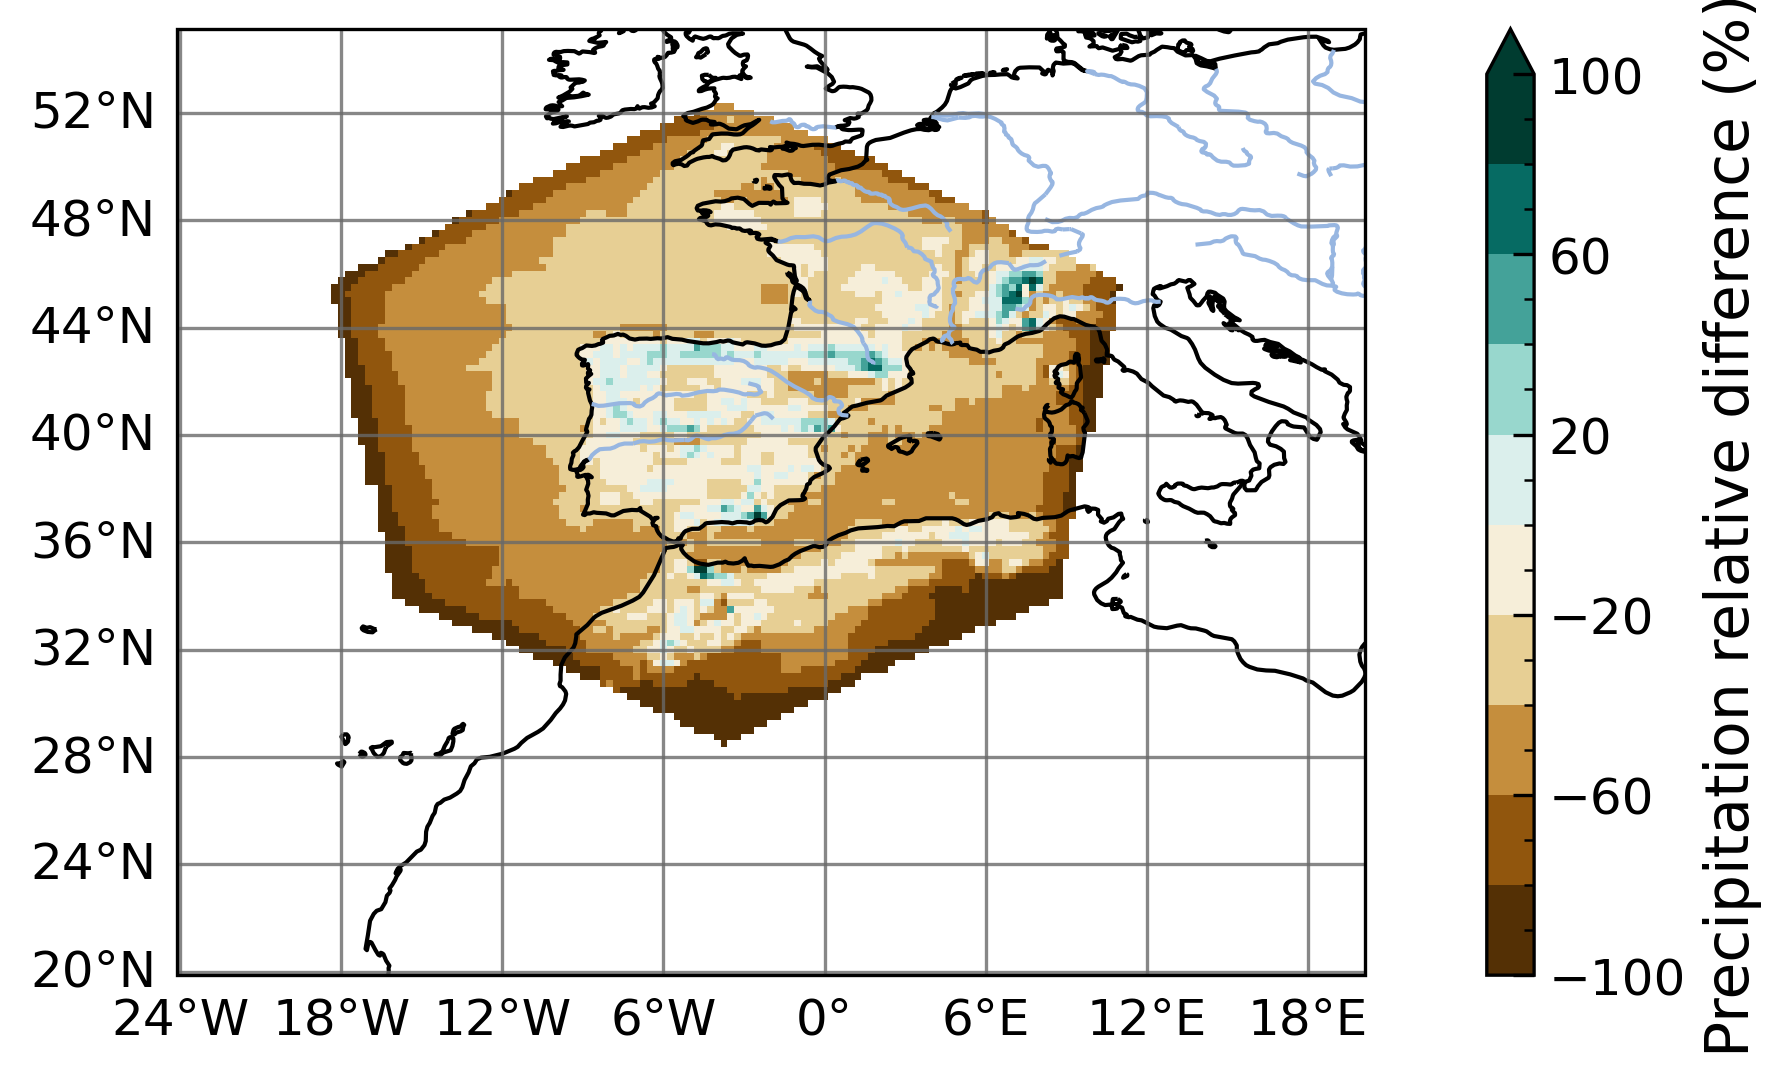
\includegraphics[width=\textwidth]{images/chap4/domain_size/rel_diff_map_precip_era_LAM_1500km_NBP60.png}
        \end{subfigure} &
        \begin{subfigure}[b]{0.33\textwidth}
            \caption{}
            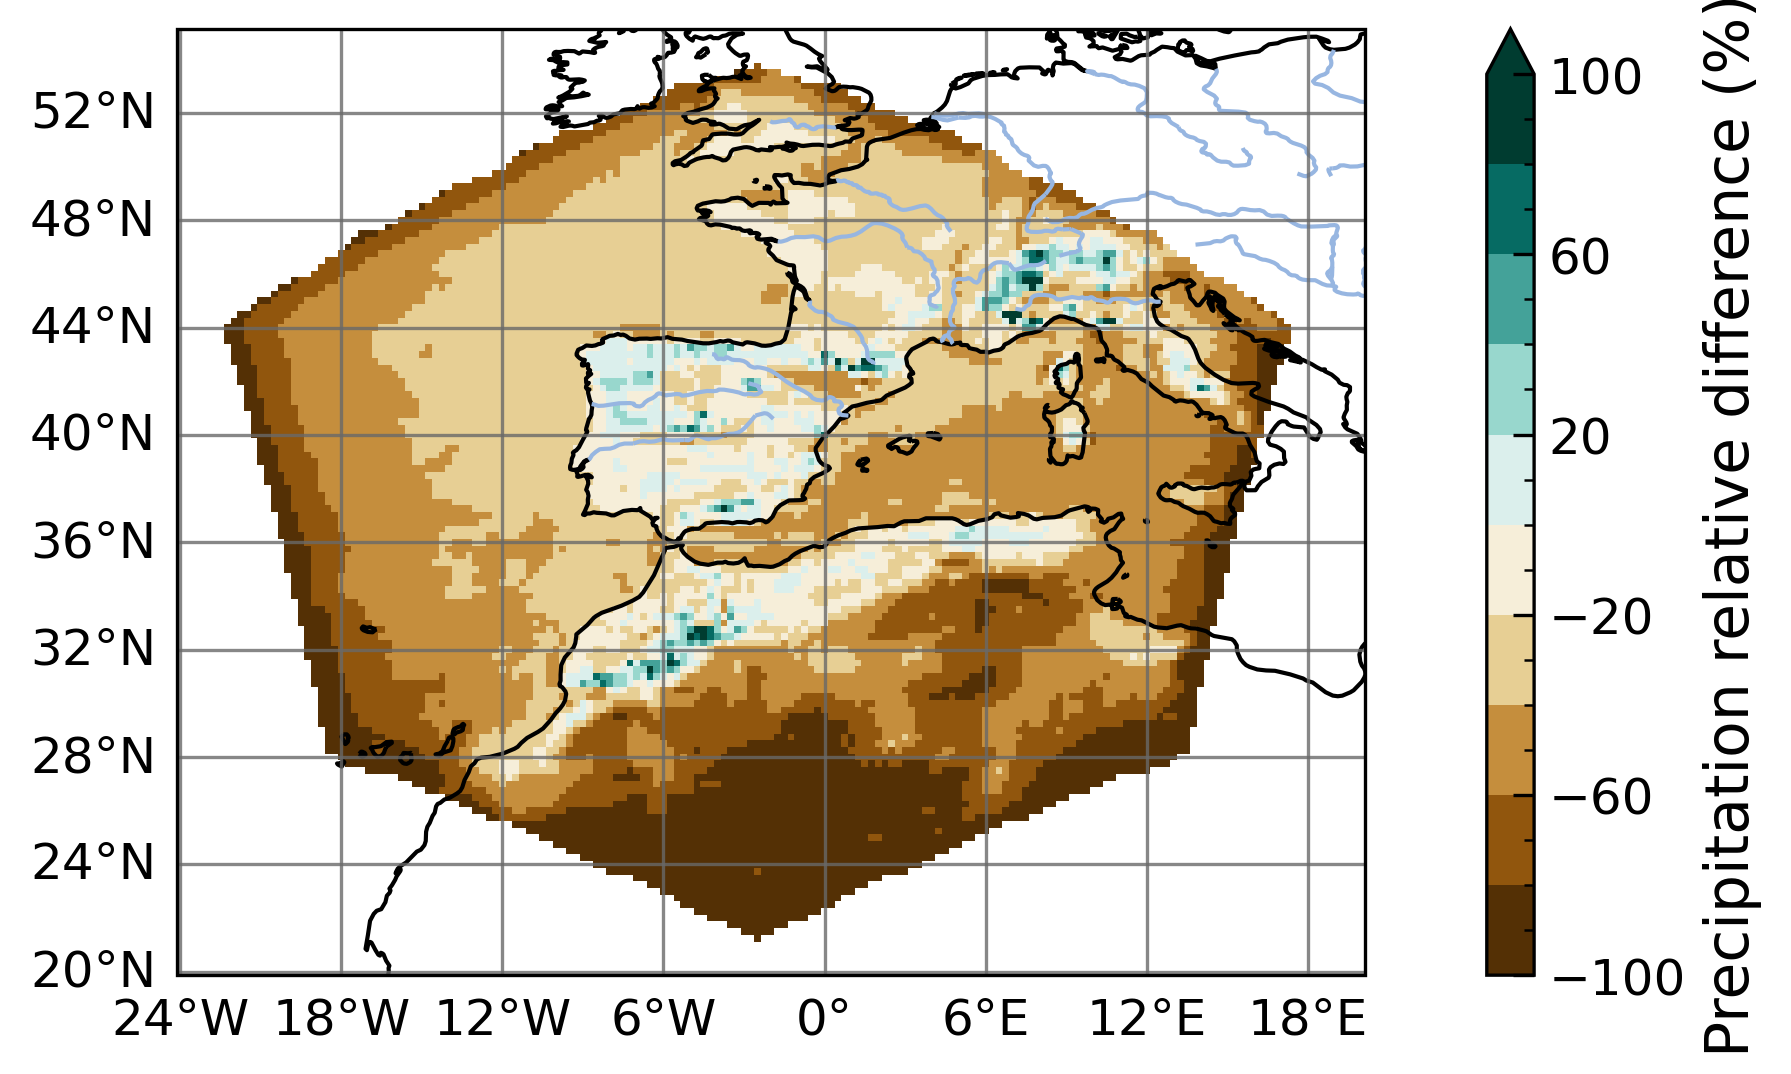
\includegraphics[width=\textwidth]{images/chap4/domain_size/rel_diff_map_precip_era_LAM_2000km_NBP80.png}
        \end{subfigure} \\
        
        %evap
        \begin{subfigure}[b]{0.33\textwidth}
            \caption{}
            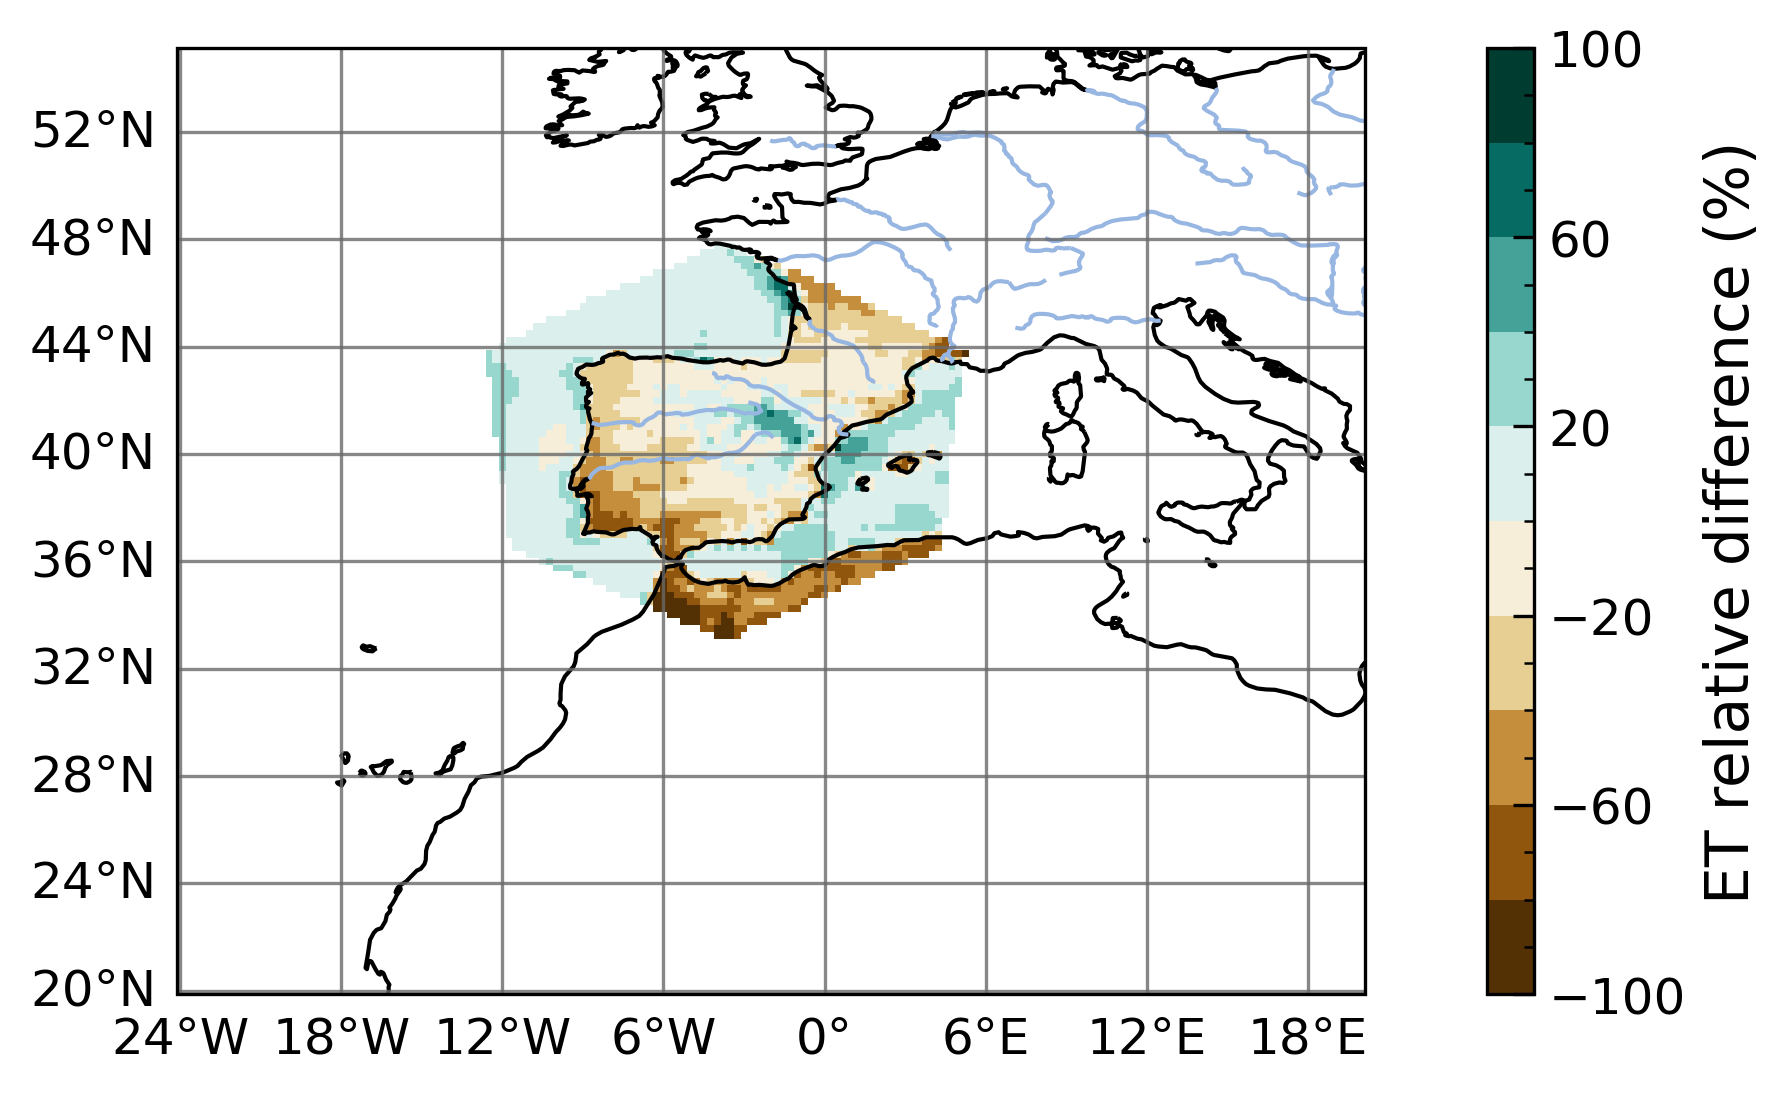
\includegraphics[width=\textwidth]{images/chap4/domain_size/rel_diff_map_evap_era_LAM_1000km_NBP40.png}
        \end{subfigure} &
        \begin{subfigure}[b]{0.33\textwidth}
            \caption{}
            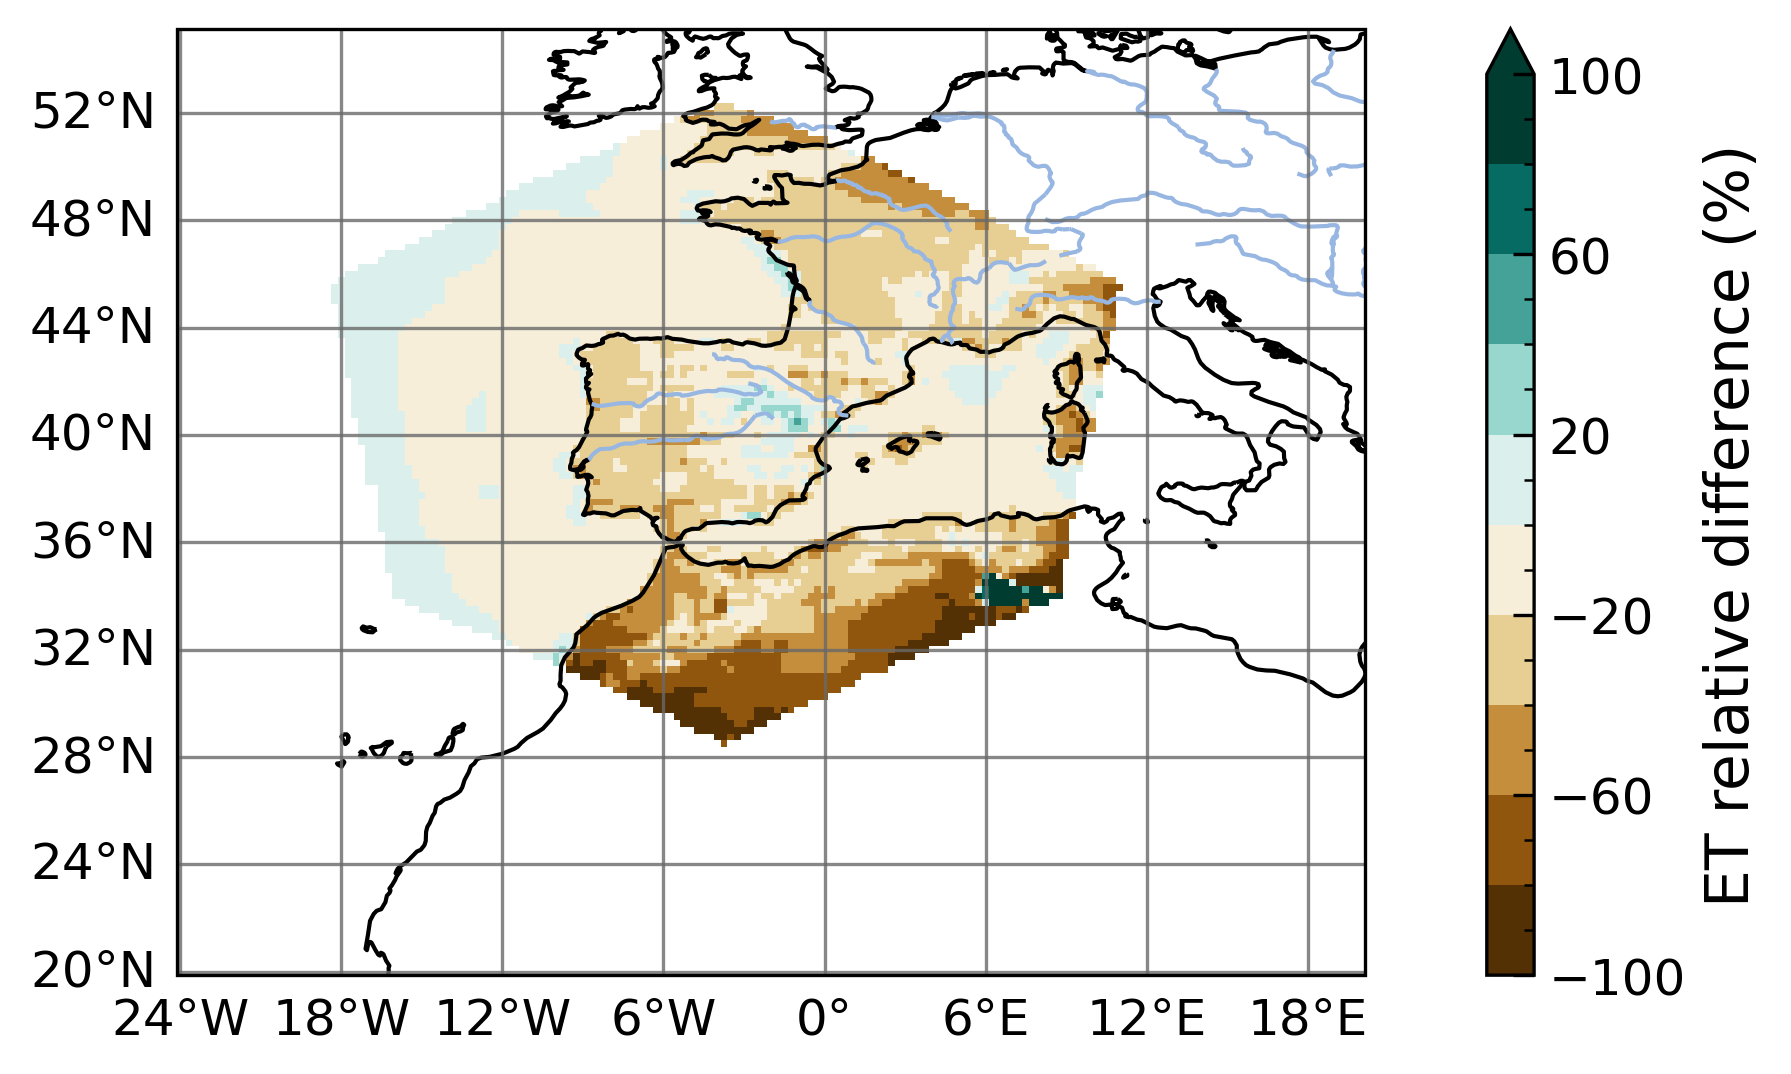
\includegraphics[width=\textwidth]{images/chap4/domain_size/rel_diff_map_evap_era_LAM_1500km_NBP60.png}
        \end{subfigure} &
        \begin{subfigure}[b]{0.33\textwidth}
            \caption{}
            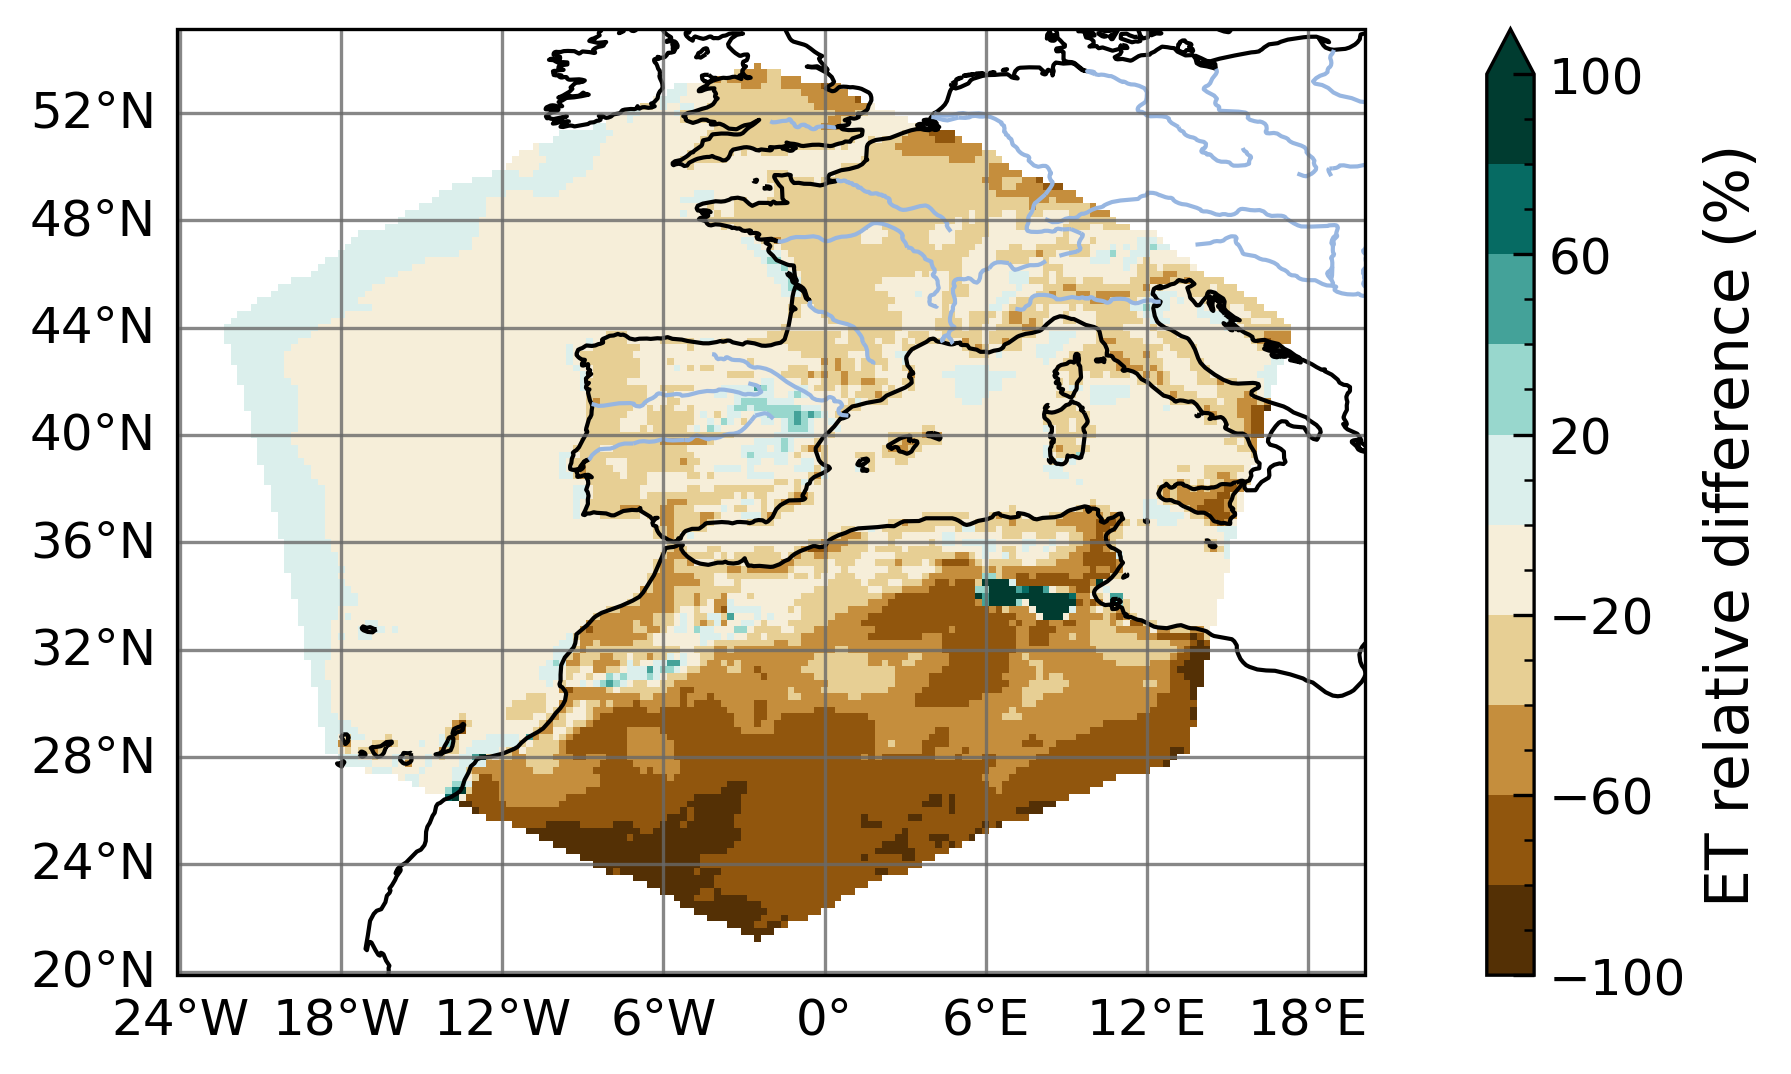
\includegraphics[width=\textwidth]{images/chap4/domain_size/rel_diff_map_evap_era_LAM_2000km_NBP80.png}
        \end{subfigure}
    \end{tabular}
    \caption{}
    \label{fig:domain_size_ERA_reldiff_maps}
\end{figure}
 
\section{Chapter \ref{chap:monthly}}
% Article

%f
\begin{figure}[htbp]
    \centering
    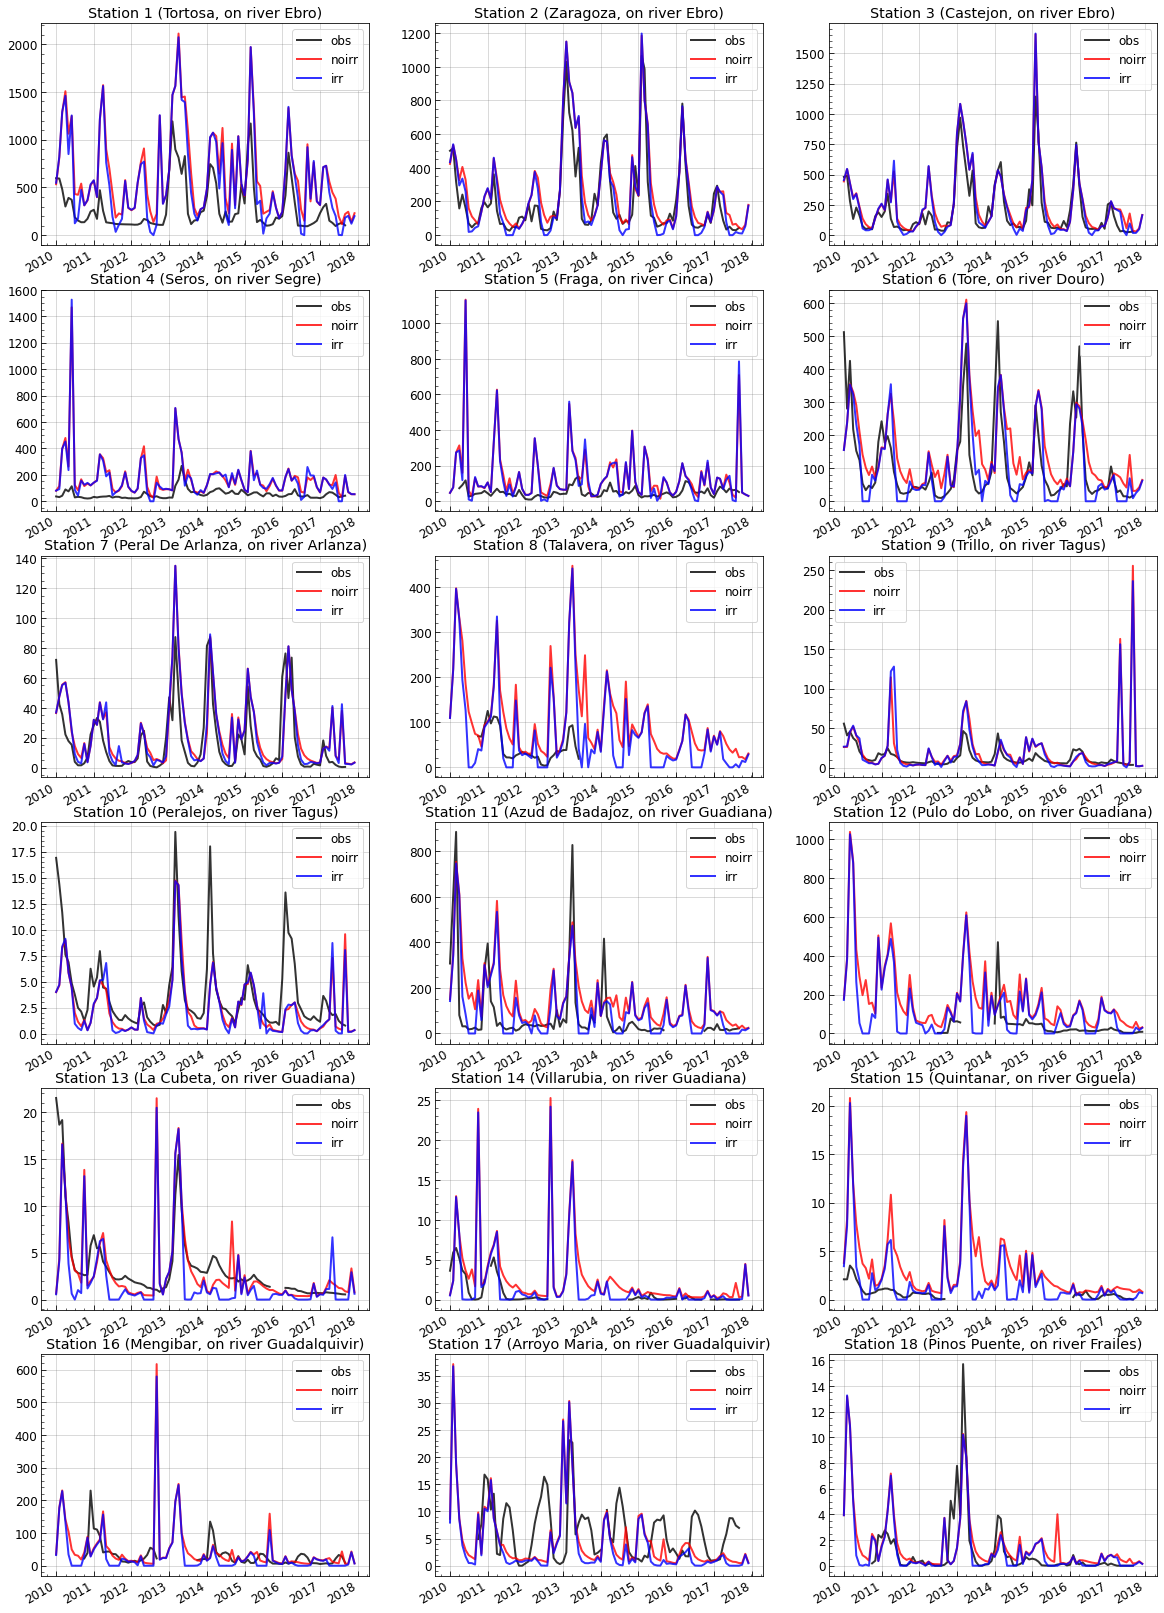
\includegraphics[width=\textwidth]{images/chap4/article/18_stations_TS.png}
    \caption{Time series of river discharge for the \irr and \noirr simulations and GRDC observations.}
    \label{fig:TS_discharge_18stations}
\end{figure}

%f
\begin{figure}[htbp]
    \centering
    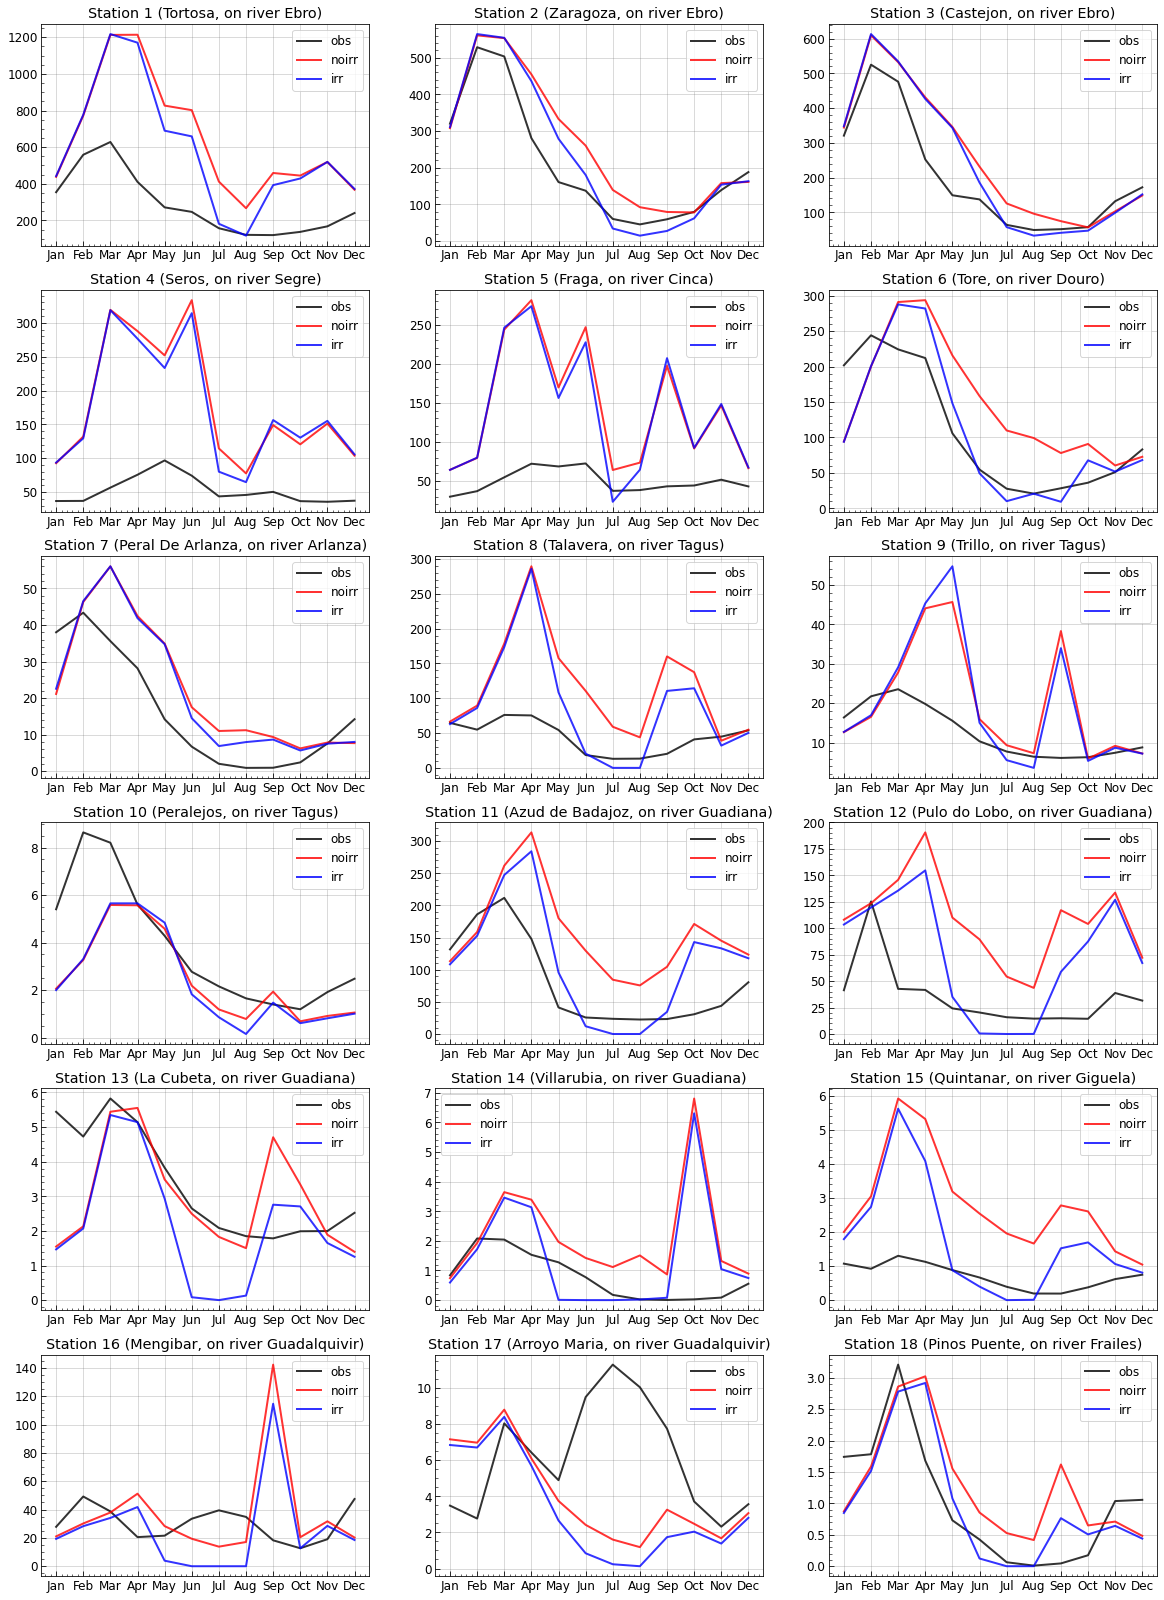
\includegraphics[width=\textwidth]{images/chap4/article/18_stations_SC.png}
    \caption{Mean seasonal cycle of river discharge for the \irr and \noirr simulations and GRDC observations. A mask is applied to the simulations to filter out months without corresponding observation data.}
    \label{fig:SC_discharge_18stations}
\end{figure}


% Climate change 

%figure : from chap 4 future vs present. Seasonnal cycle of variables for 3 sims
\begin{figure}[htbp]
    \centering
    \begin{tabular}{cc}
        %precip
        \begin{subfigure}[b]{0.5\textwidth}
            \caption{}
            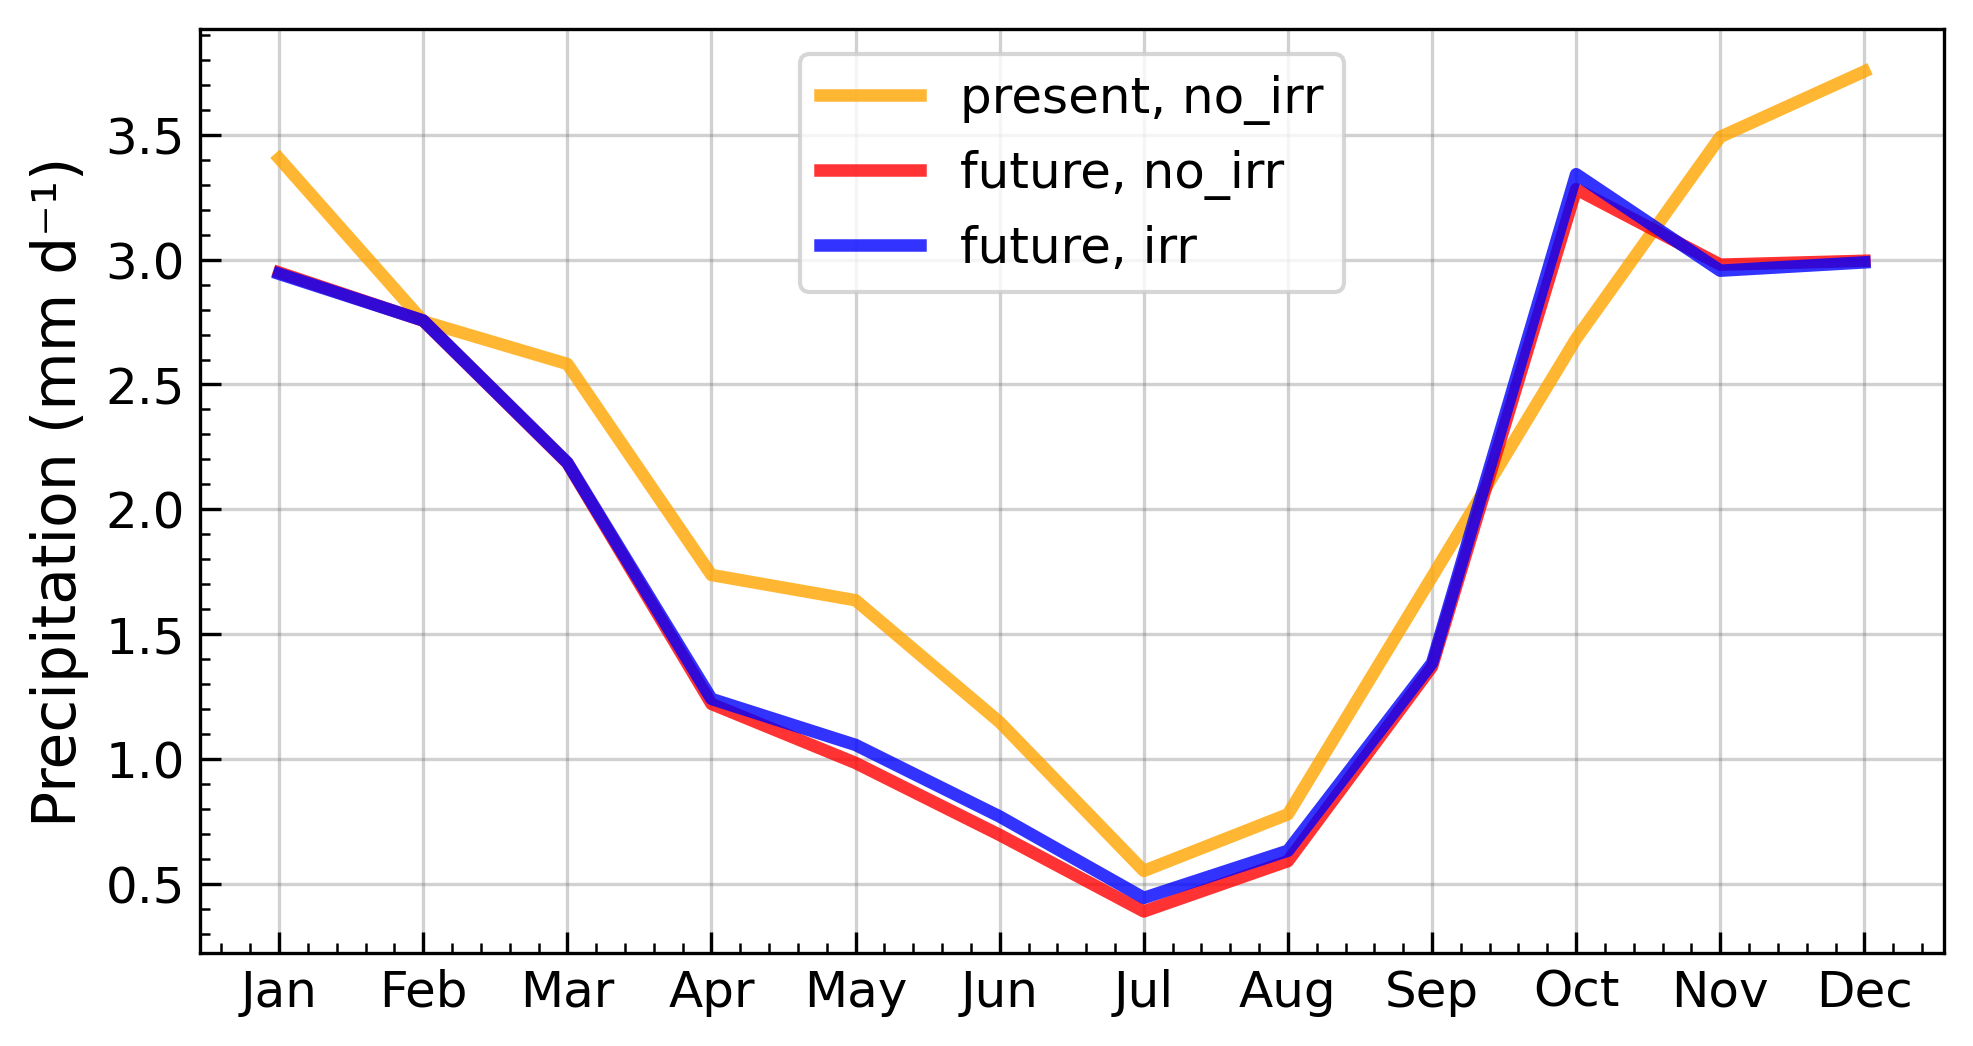
\includegraphics[width=\textwidth]{images/chap4/future/SC_precip_presfutirr.png}
        \end{subfigure} &
        %evap
        \begin{subfigure}[b]{0.5\textwidth}
            \caption{}
            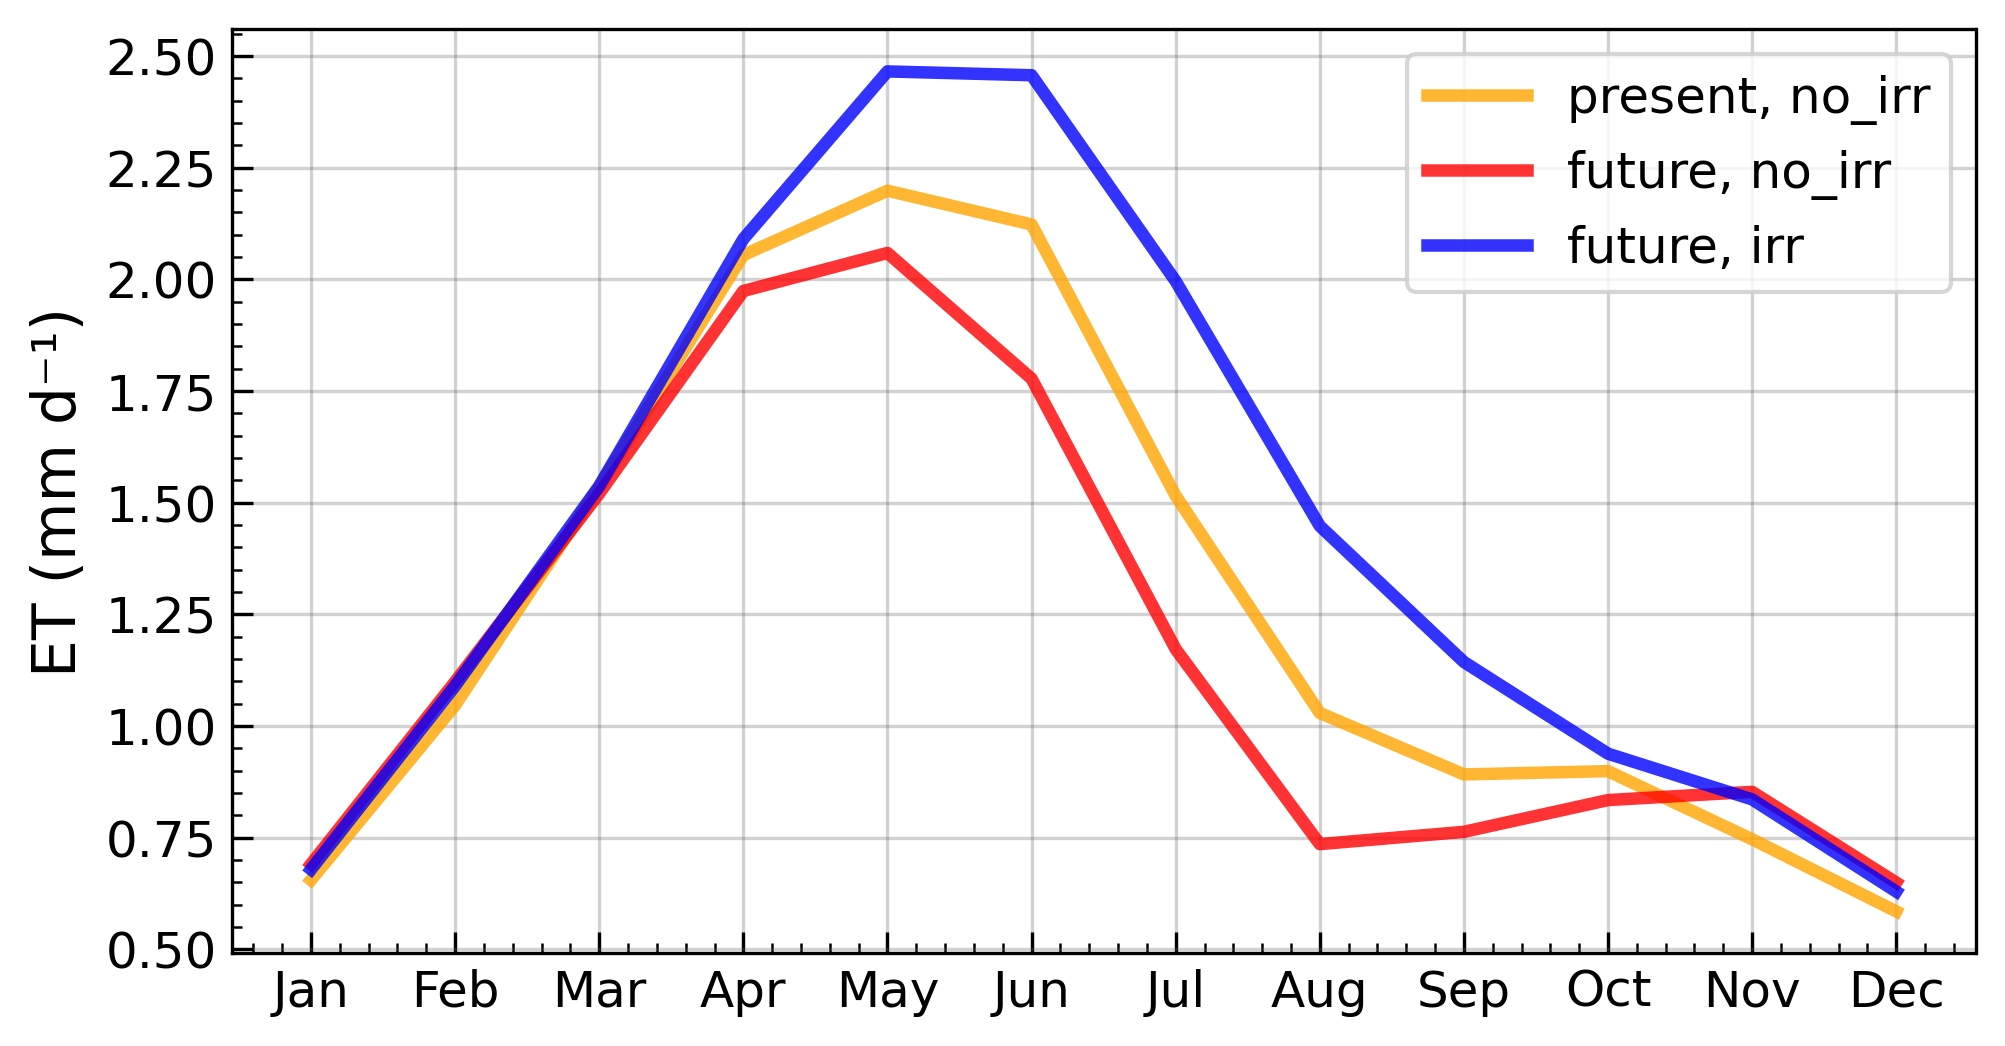
\includegraphics[width=\textwidth]{images/chap4/future/SC_evap_presfutirr.png}
        \end{subfigure} \\

        %t2m
        \begin{subfigure}[b]{0.5\textwidth}
            \caption{}
            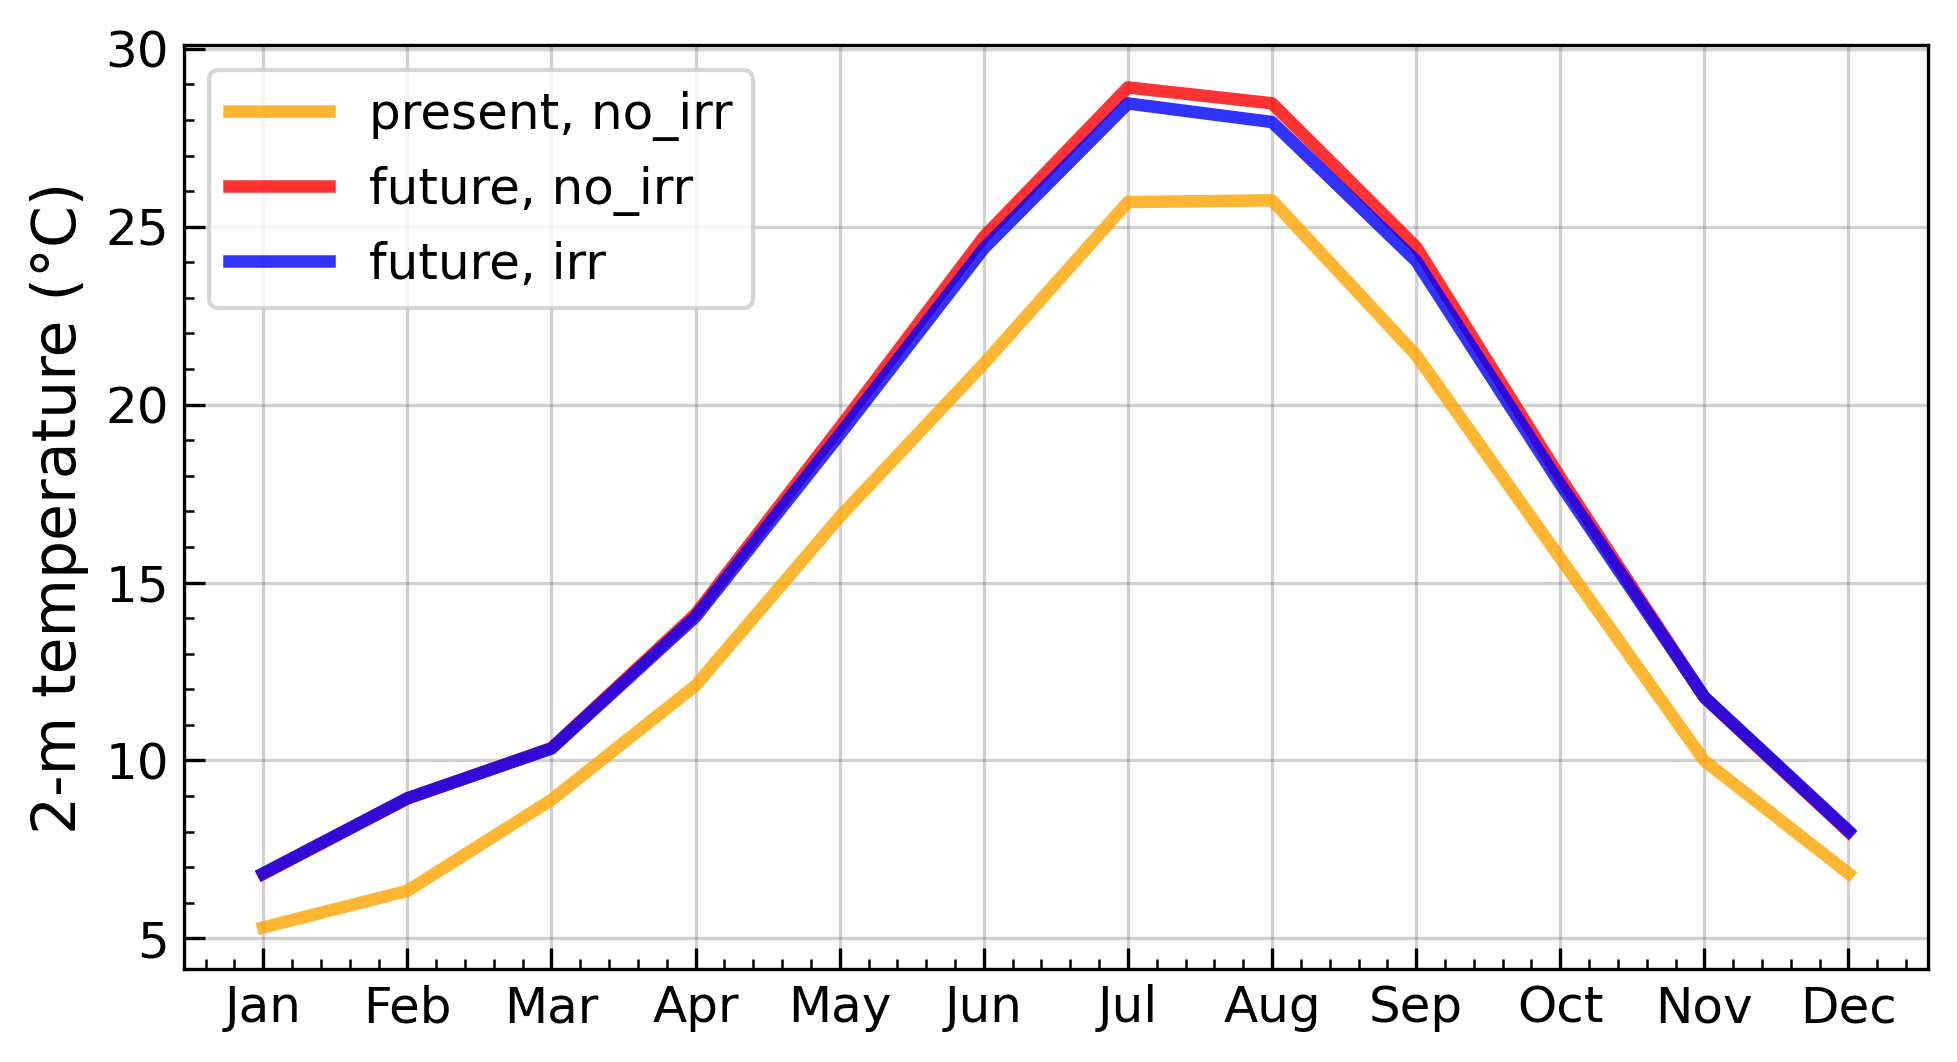
\includegraphics[width=\textwidth]{images/chap4/future/SC_t2m_presfutirr.png}
        \end{subfigure} &
        %fluxsens
        \begin{subfigure}[b]{0.5\textwidth}
            \caption{}
            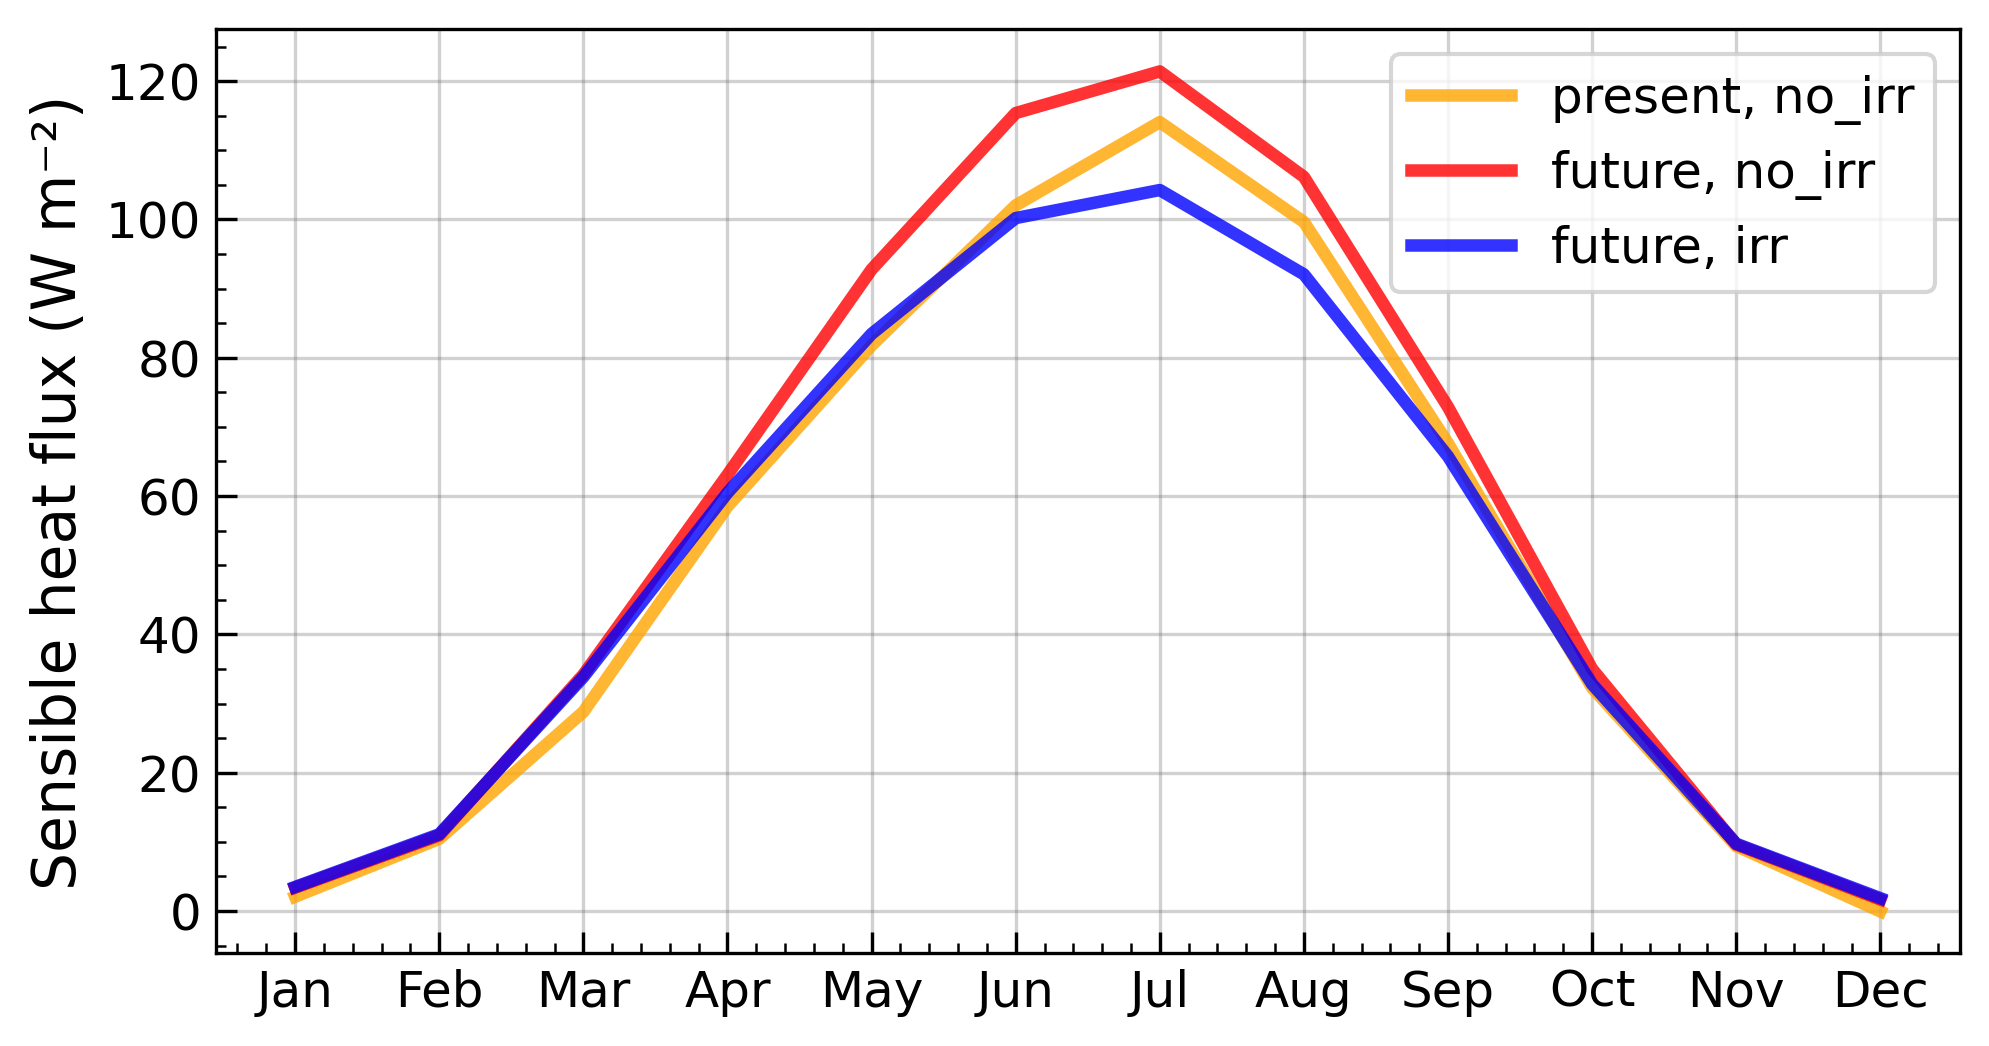
\includegraphics[width=\textwidth]{images/chap4/future/SC_fluxsens_presfutirr.png}
        \end{subfigure} \\

        %q2m
        \begin{subfigure}[b]{0.5\textwidth}
            \caption{}
            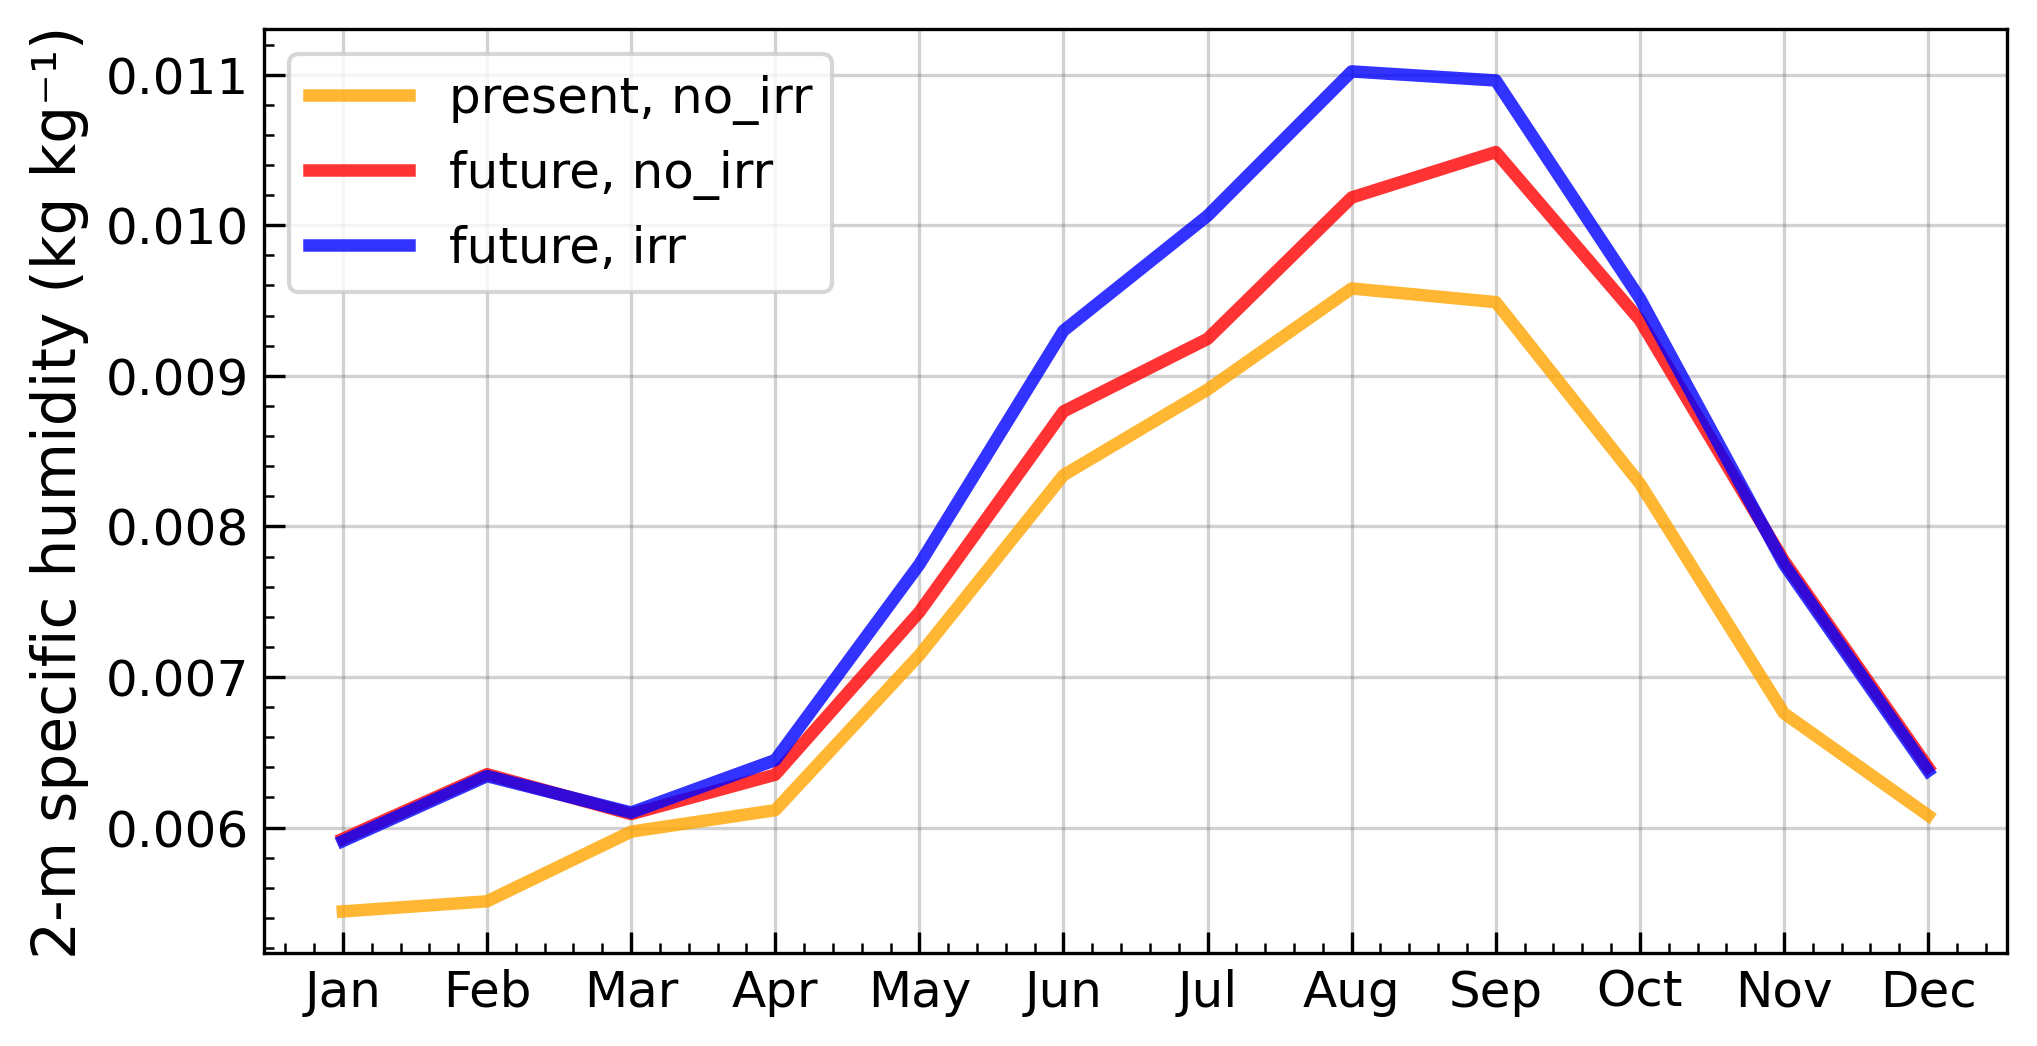
\includegraphics[width=\textwidth]{images/chap4/future/SC_q2m_presfutirr.png}
        \end{subfigure} &
        %rh2m
        \begin{subfigure}[b]{0.5\textwidth}
            \caption{}
            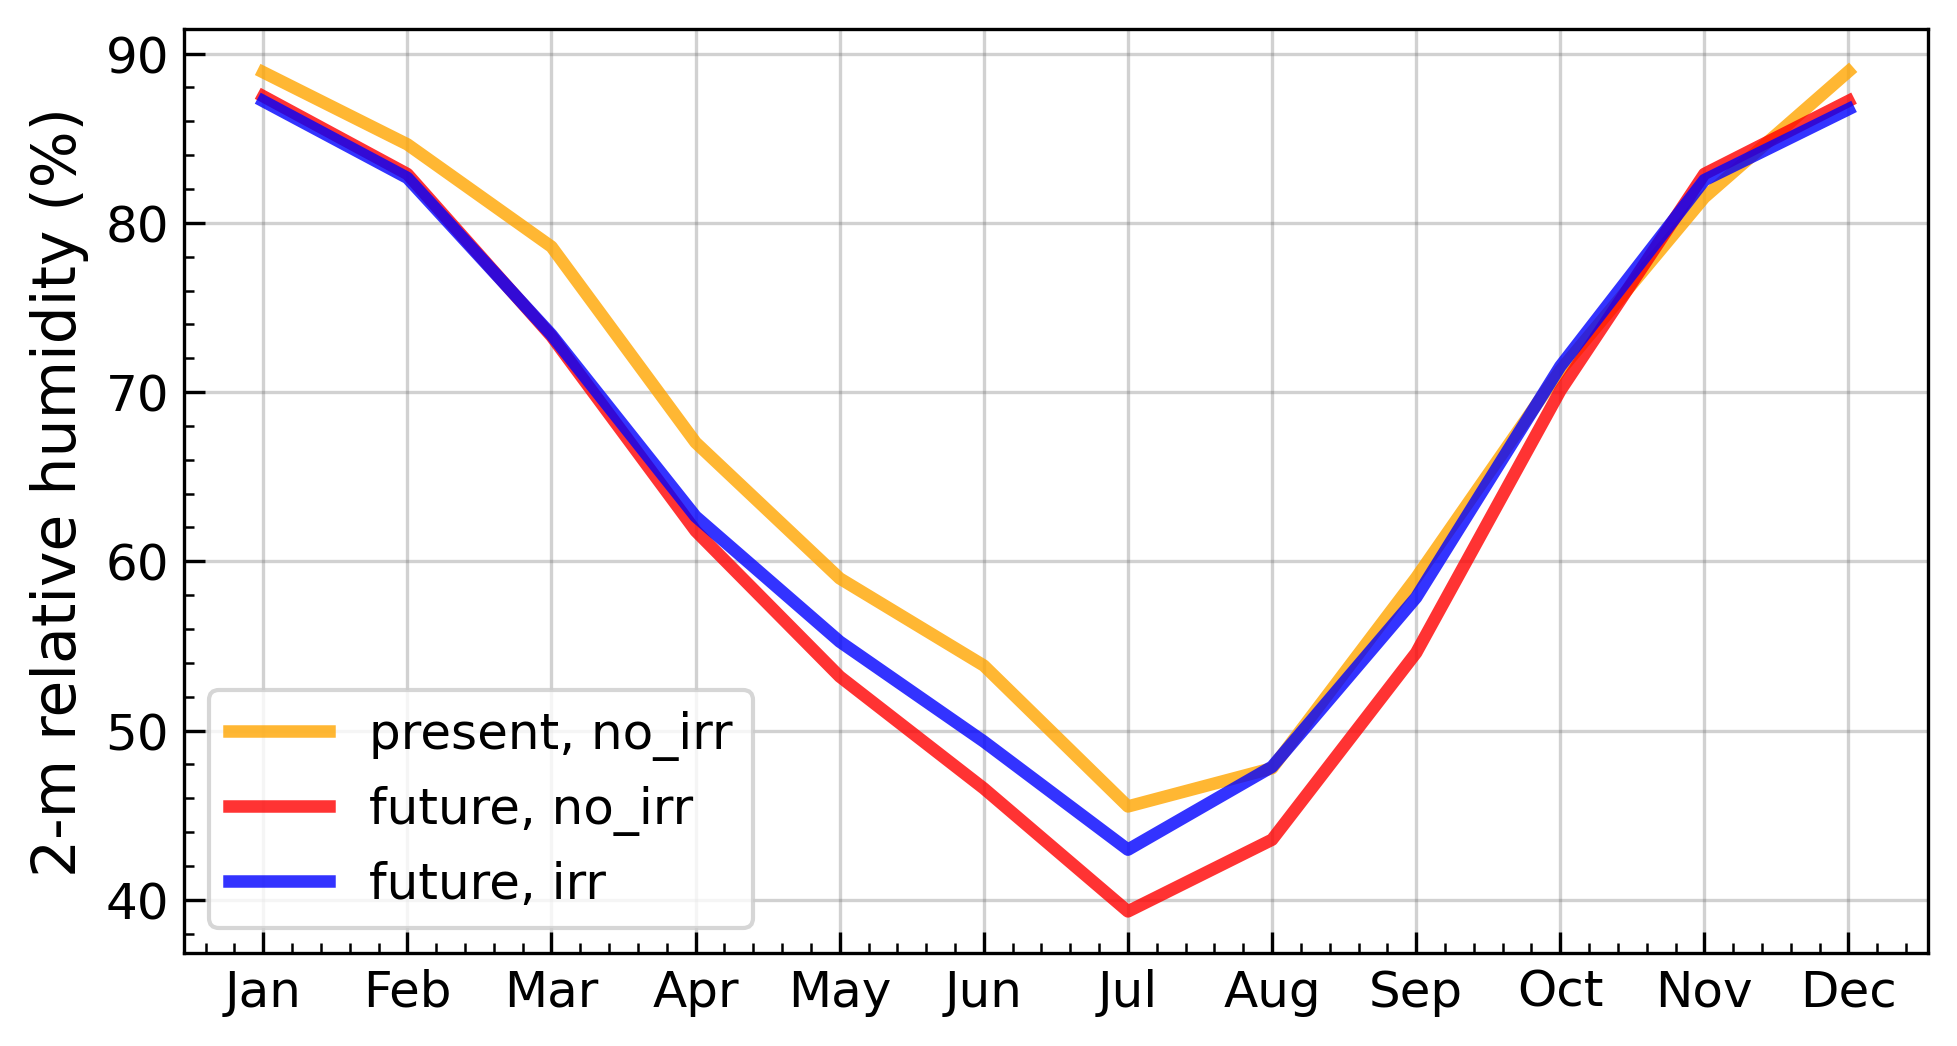
\includegraphics[width=\textwidth]{images/chap4/future/SC_rh2m_presfutirr.png}
        \end{subfigure} \\

        %pblh
        \begin{subfigure}[b]{0.5\textwidth}
            \caption{}
            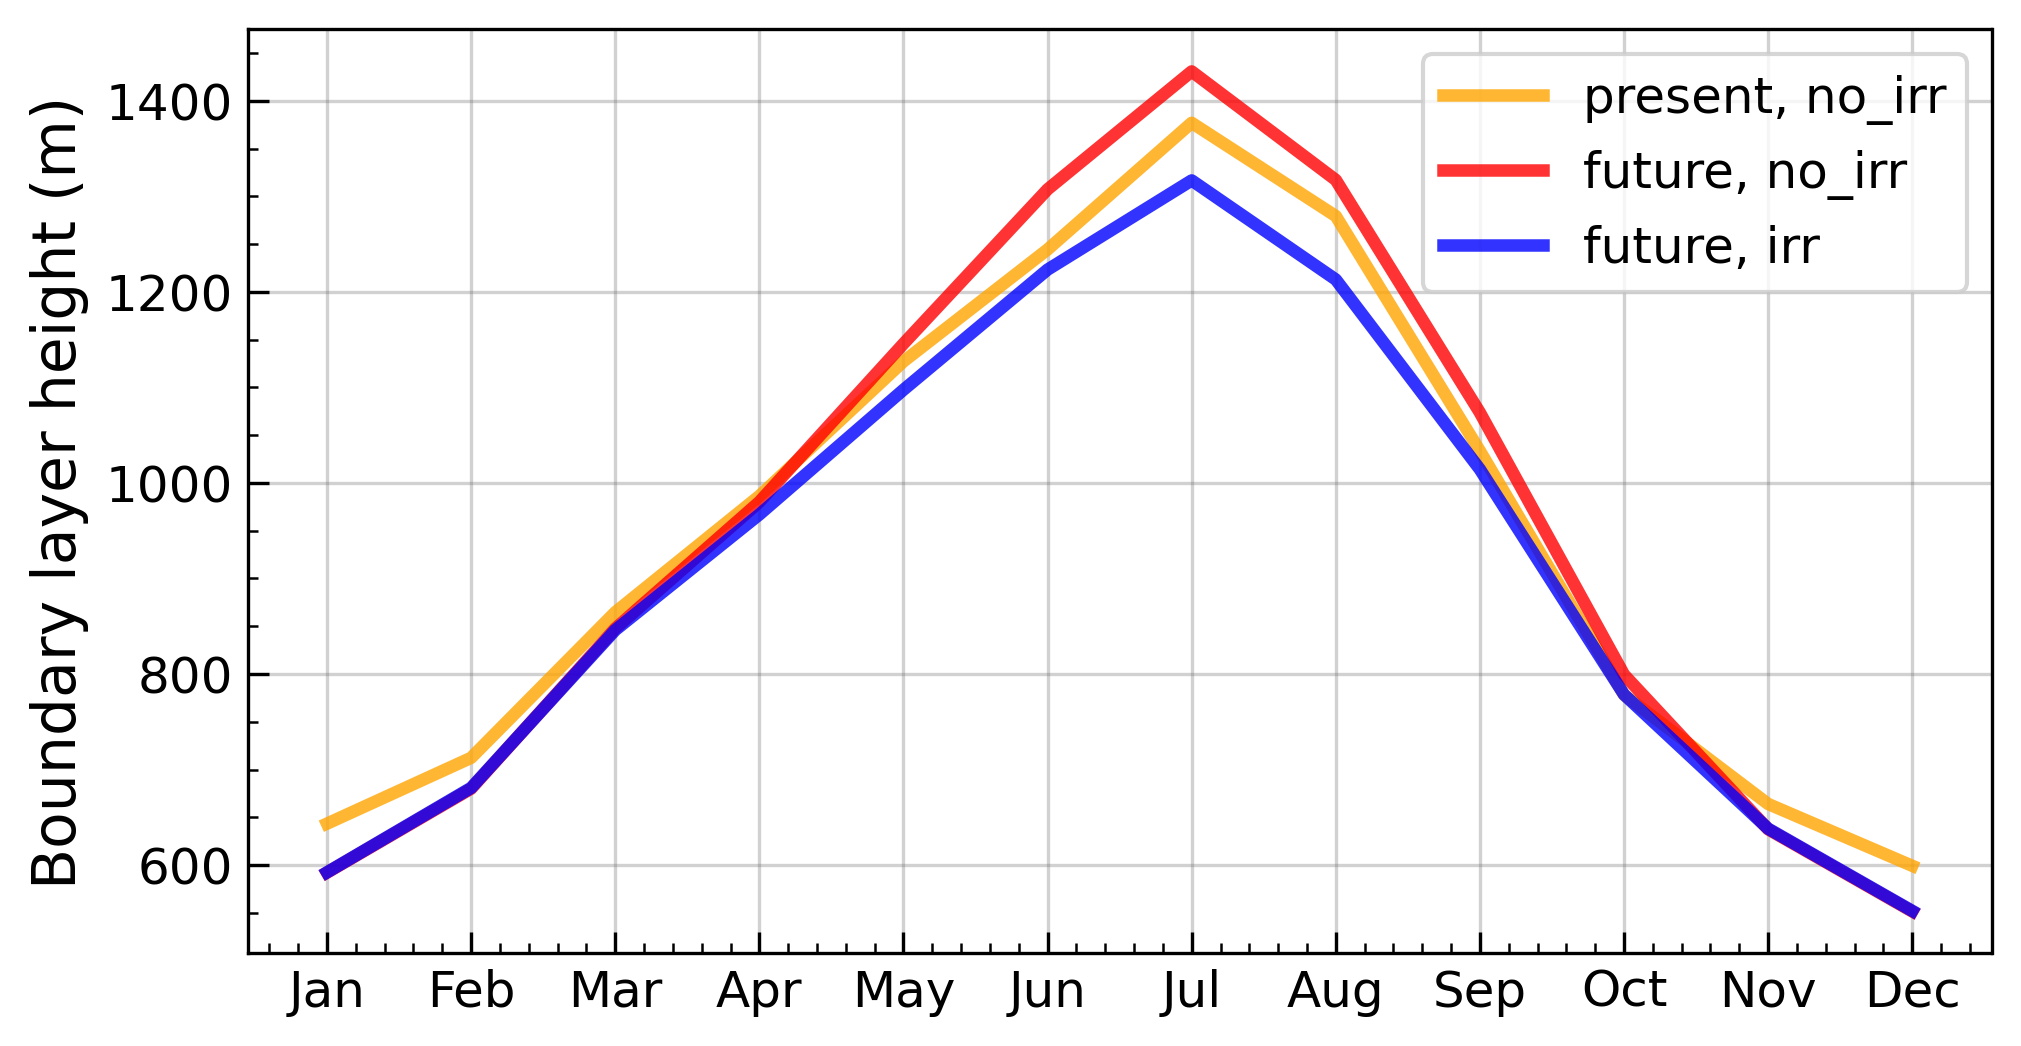
\includegraphics[width=\textwidth]{images/chap4/future/SC_s_pblh_presfutirr.png}
        \end{subfigure} &
        %lcl
        \begin{subfigure}[b]{0.5\textwidth}
            \caption{}
            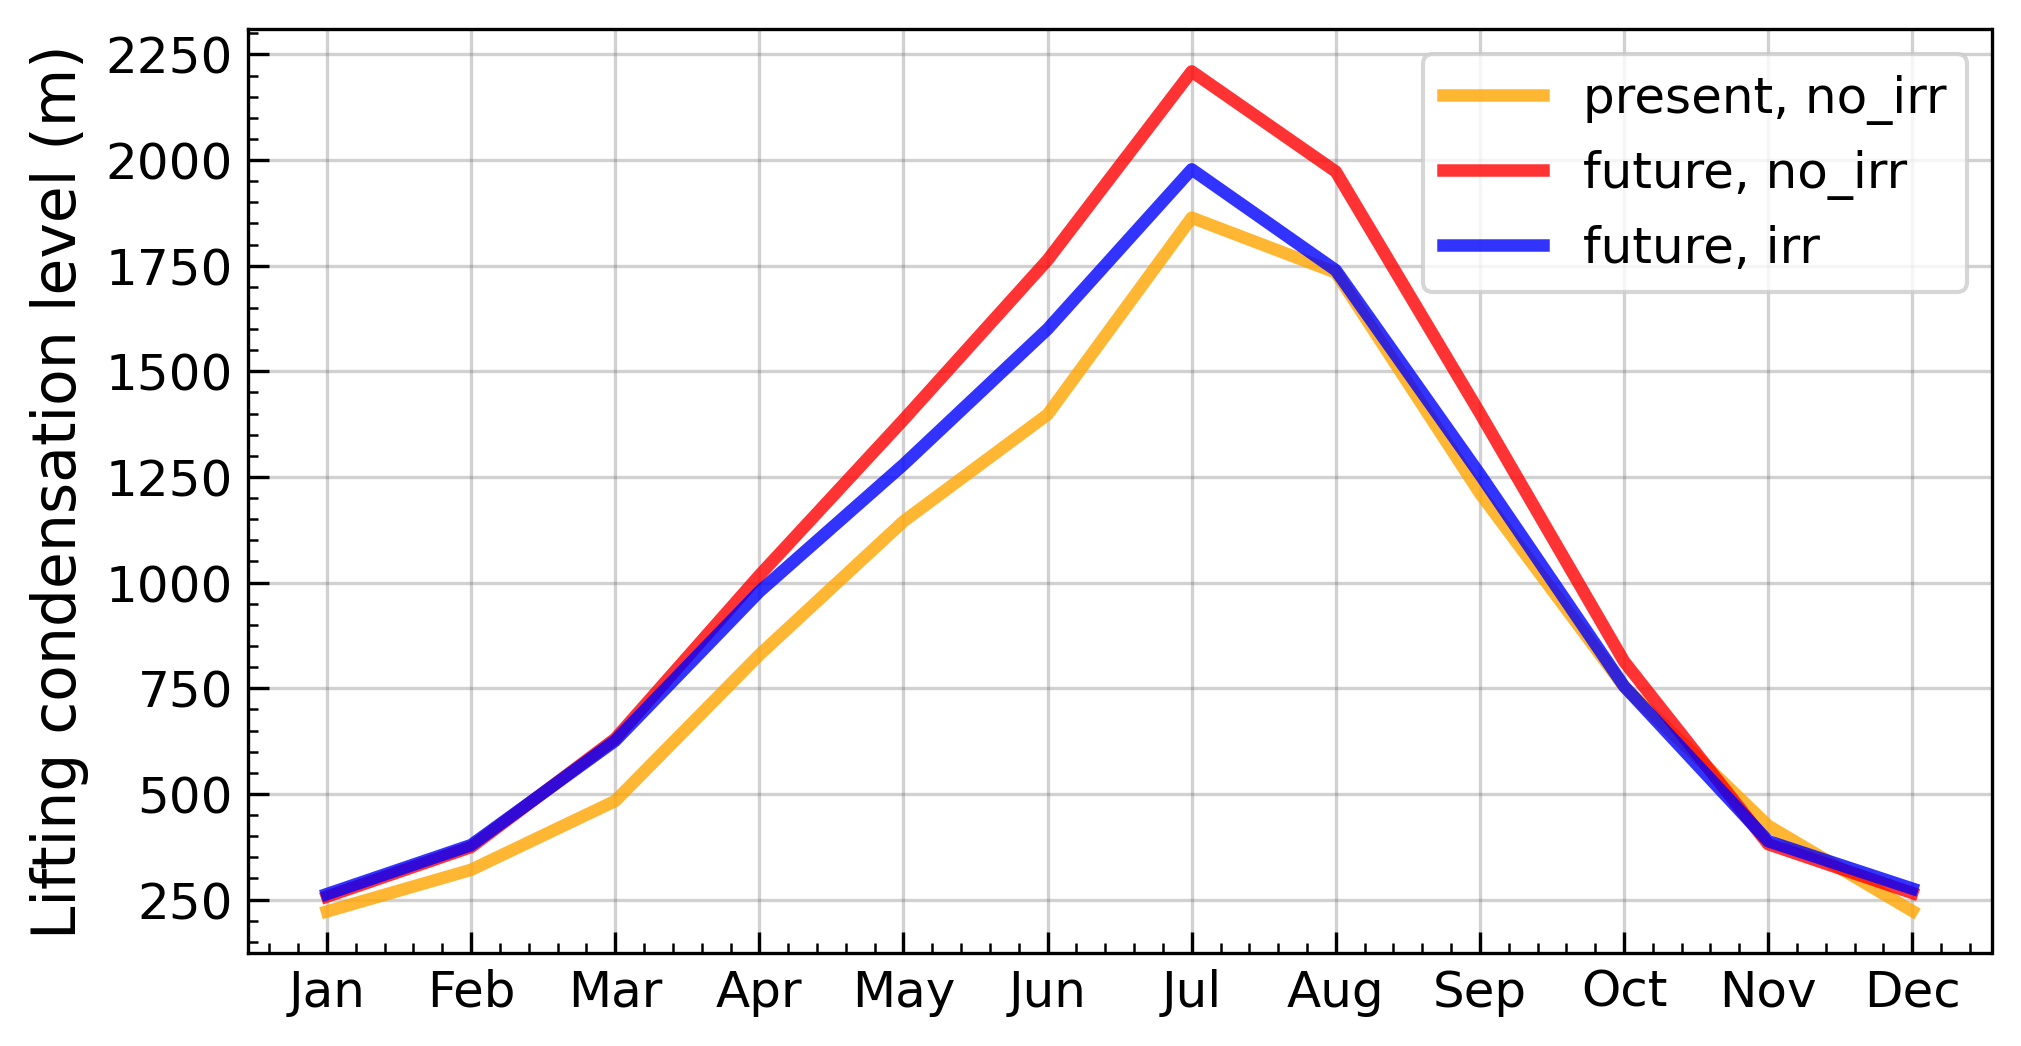
\includegraphics[width=\textwidth]{images/chap4/future/SC_s_lcl_presfutirr.png}
        \end{subfigure} \\
    \end{tabular}
    \caption{}
    \label{fig:diffmaps_future_irr}
\end{figure}

%figure : diff maps JJA (noirr, pres - future)
% \begin{figure}[htbp]
%     \centering
%     \begin{tabular}{cc}
%         %precip
%         \begin{subfigure}[b]{0.5\textwidth}
%             \caption{}
%             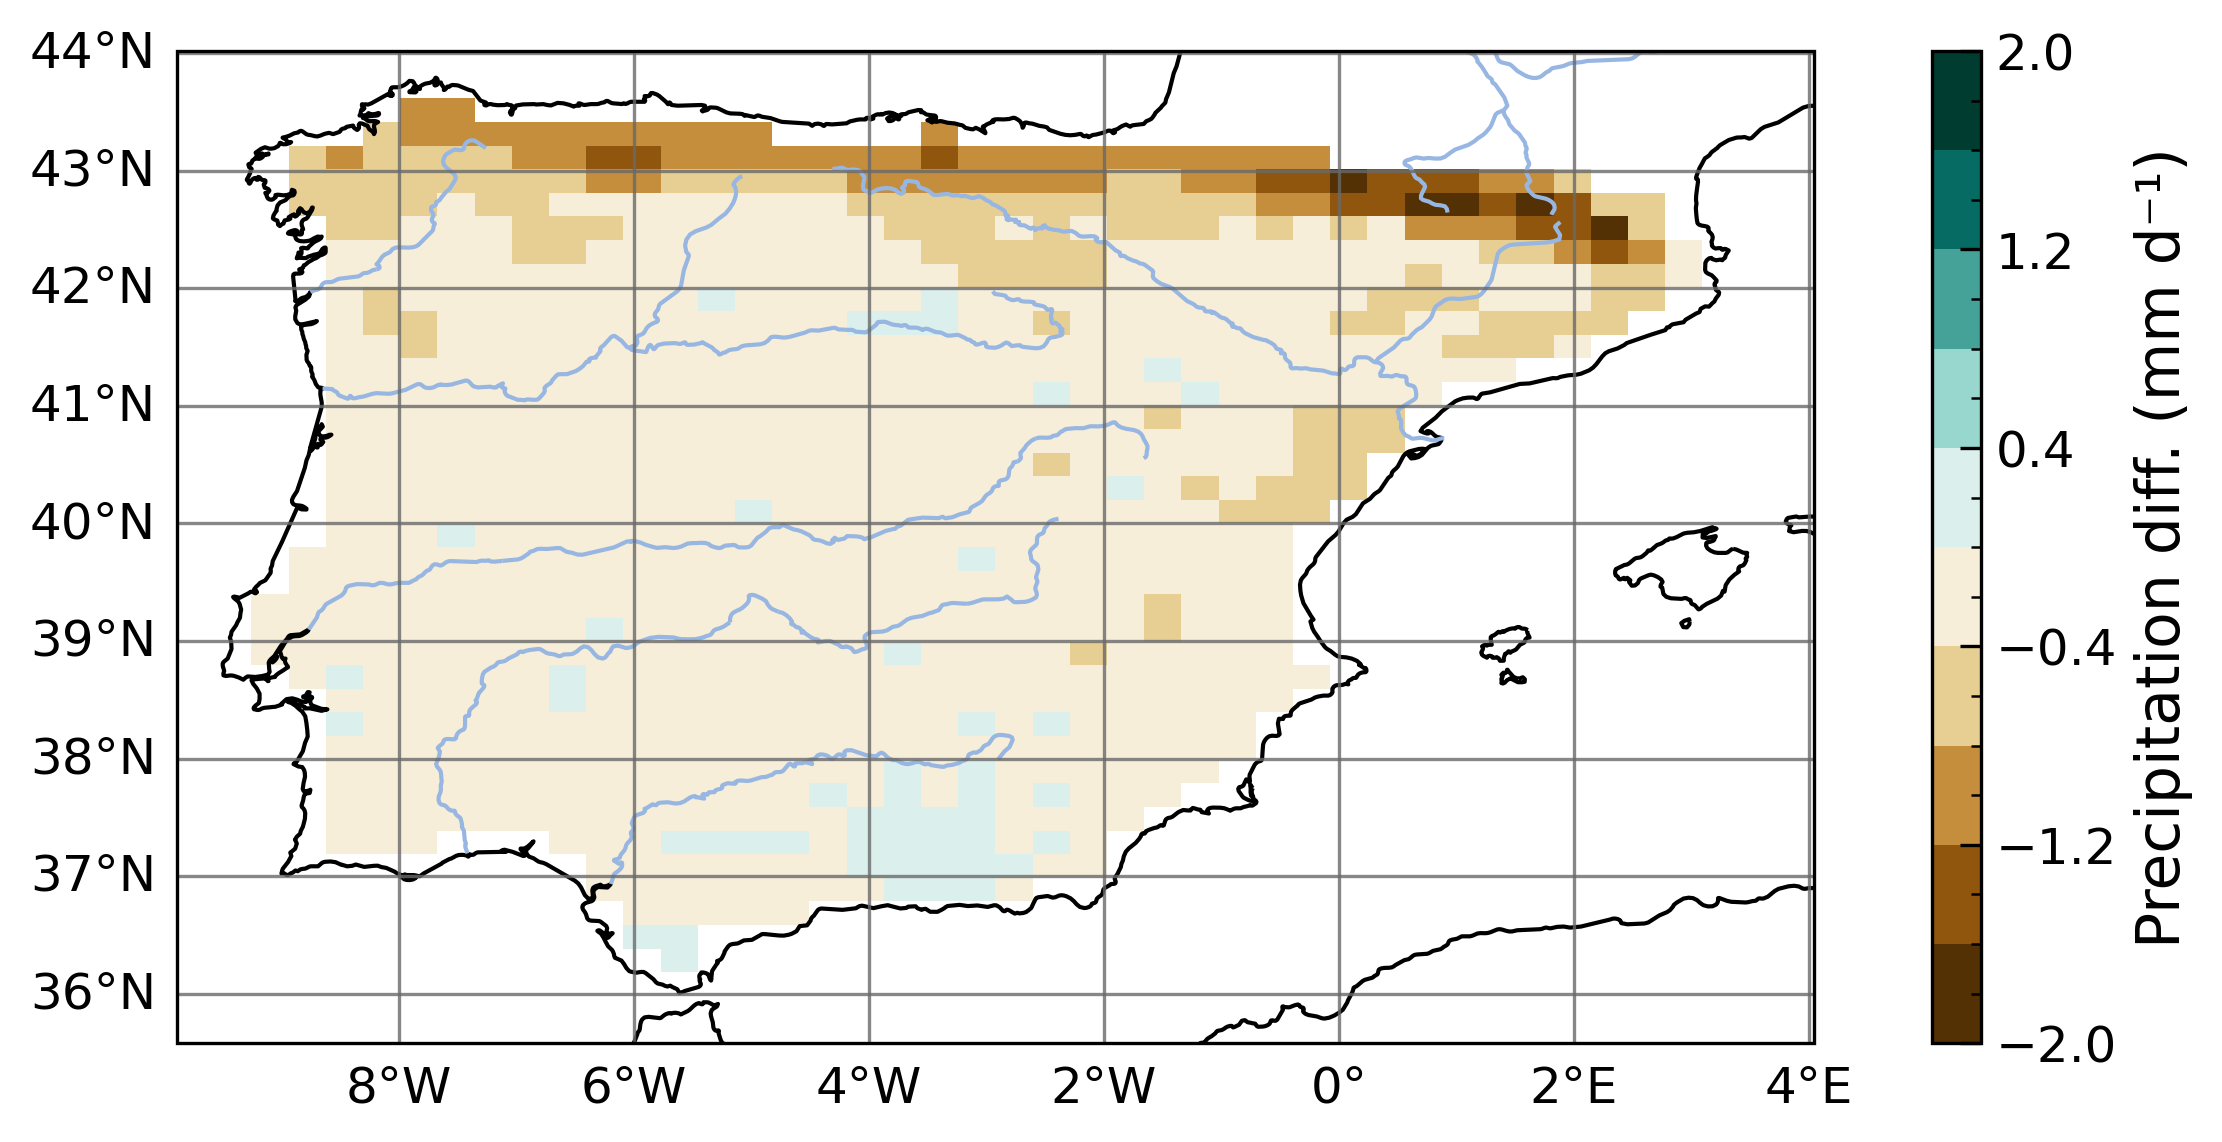
\includegraphics[width=\textwidth]{images/chap4/future/diffmap_JJA_precip_presfut.png}
%         \end{subfigure} &
%         %evap
%         \begin{subfigure}[b]{0.5\textwidth}
%             \caption{}
%             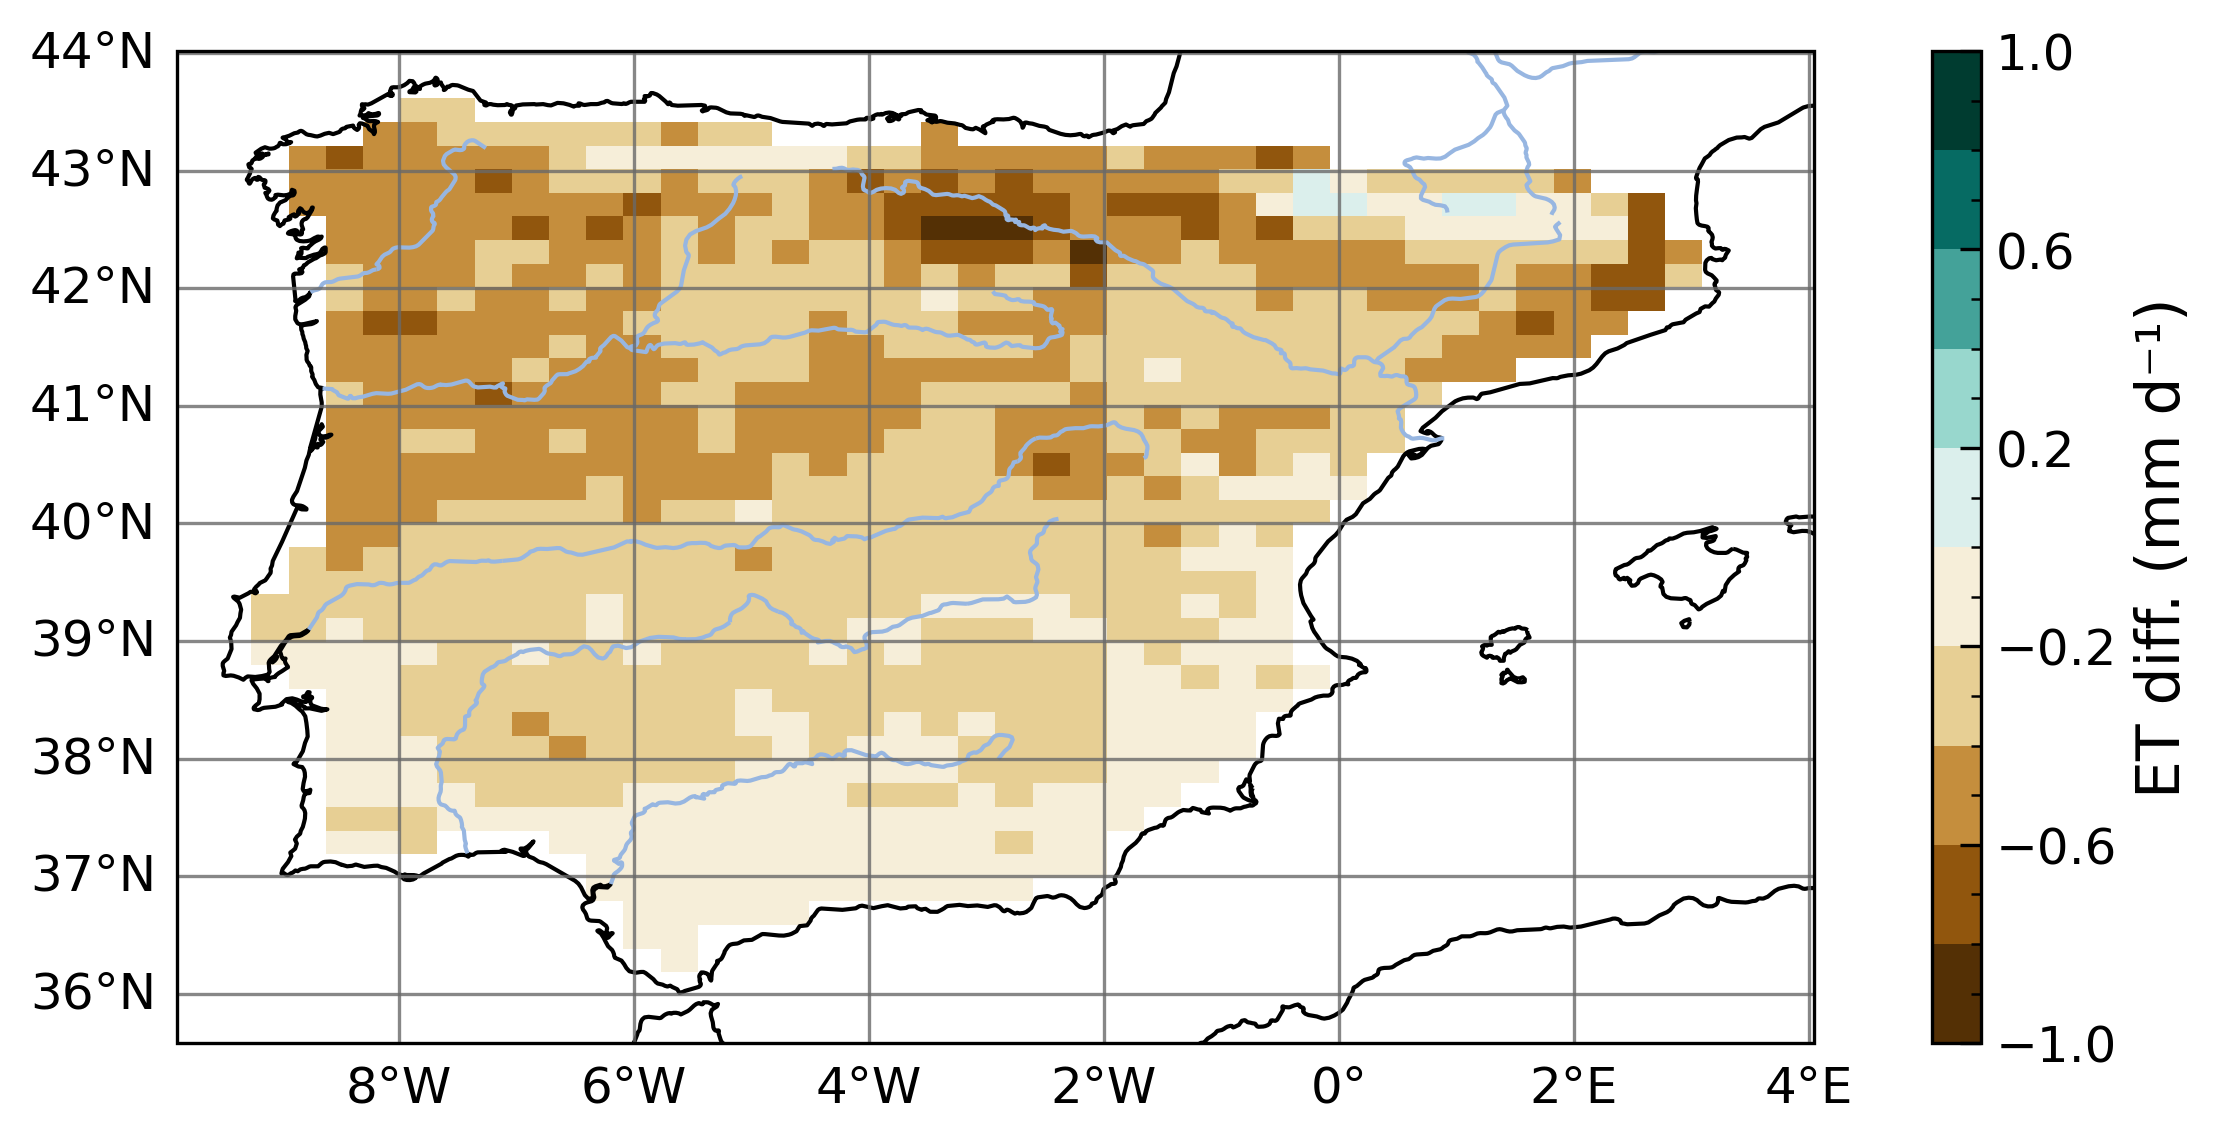
\includegraphics[width=\textwidth]{images/chap4/future/diffmap_JJA_evap_presfut.png}
%         \end{subfigure} \\

%         %t2m
%         \begin{subfigure}[b]{0.5\textwidth}
%             \caption{}
%             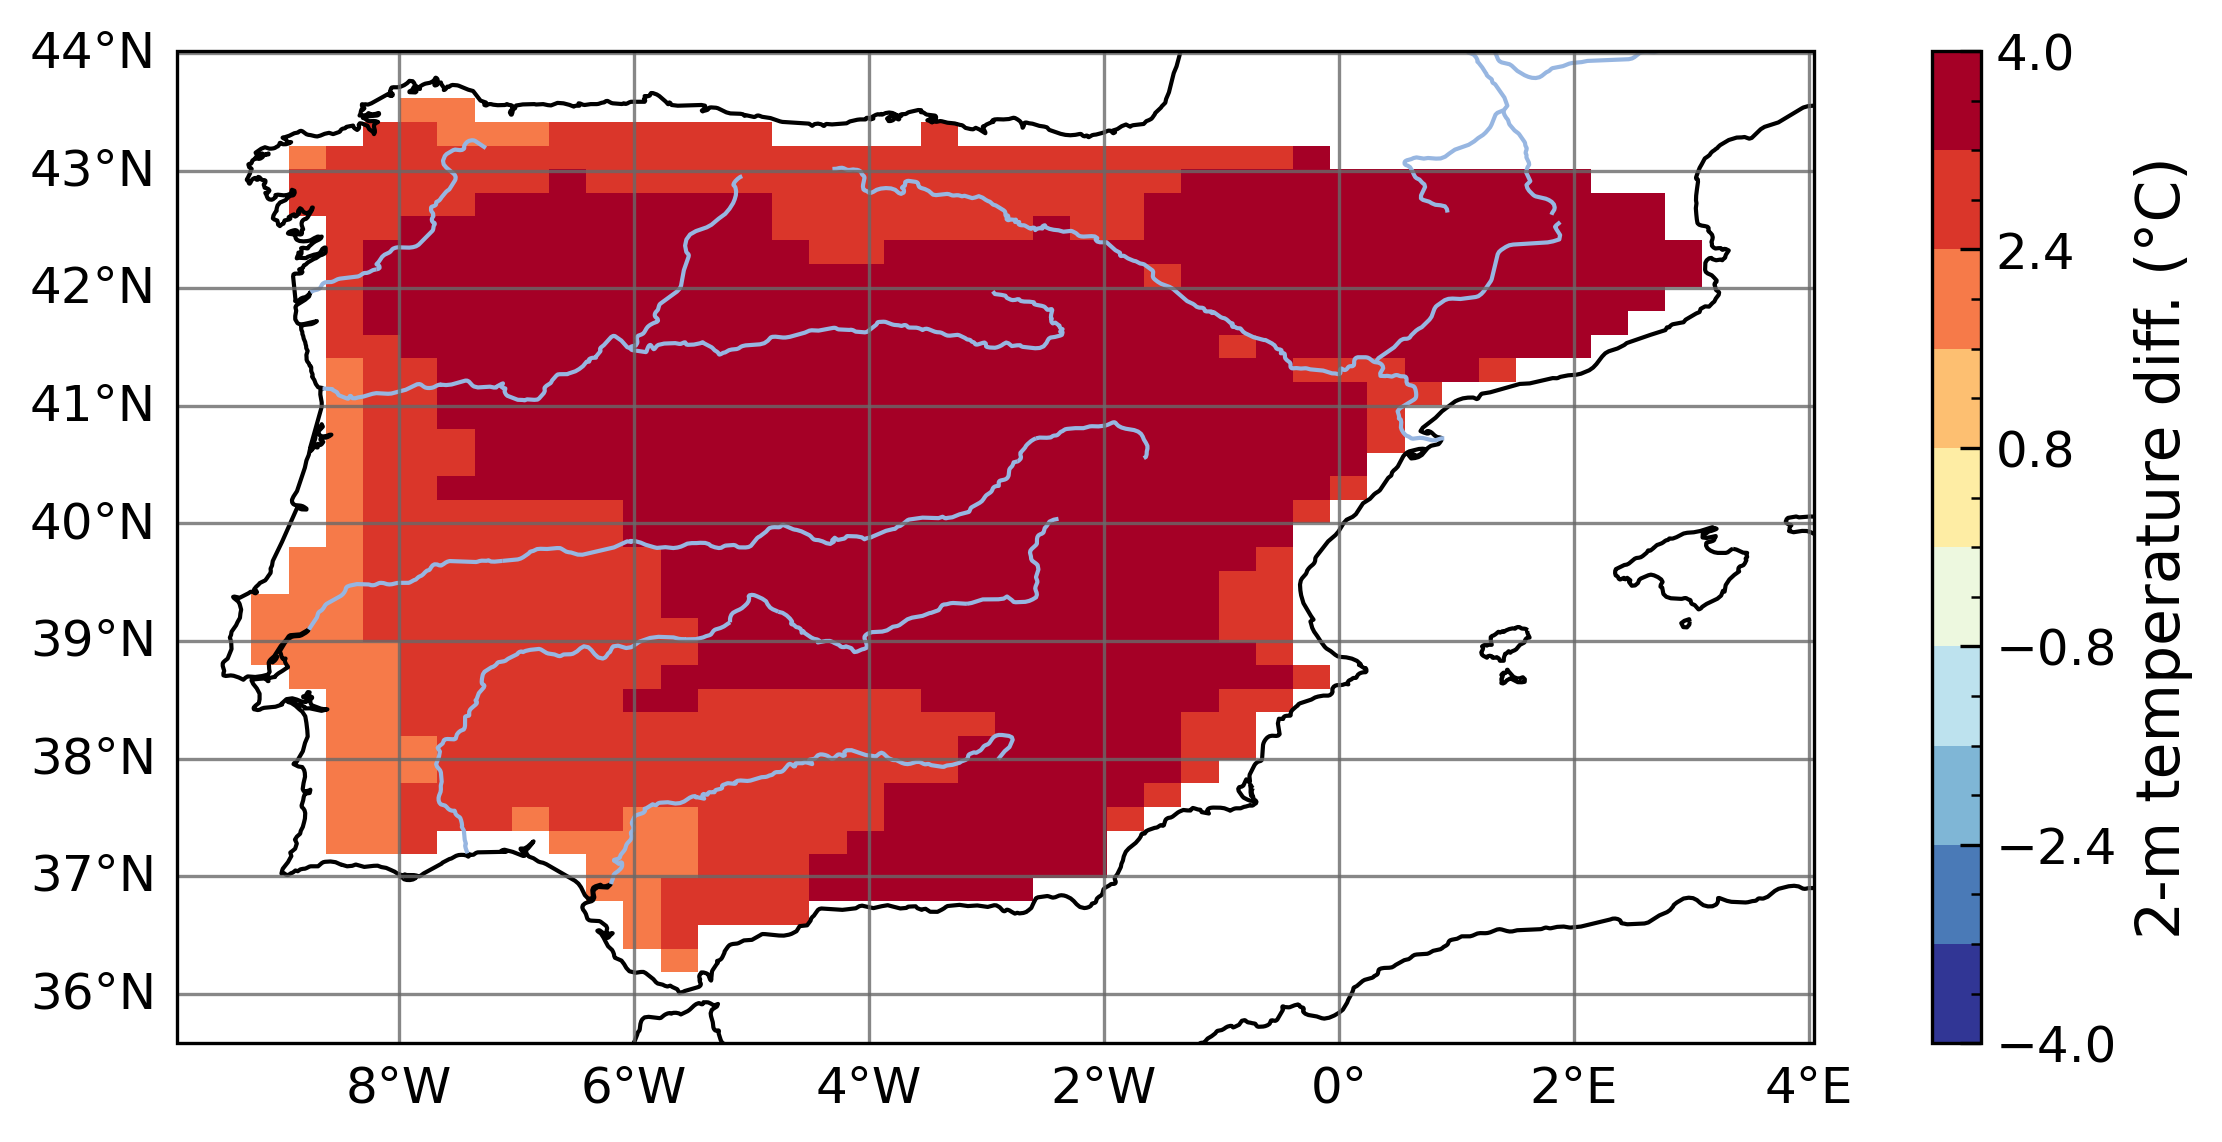
\includegraphics[width=\textwidth]{images/chap4/future/diffmap_JJA_t2m_presfut.png}
%         \end{subfigure} &
%         %fluxsens
%         \begin{subfigure}[b]{0.5\textwidth}
%             \caption{}
%             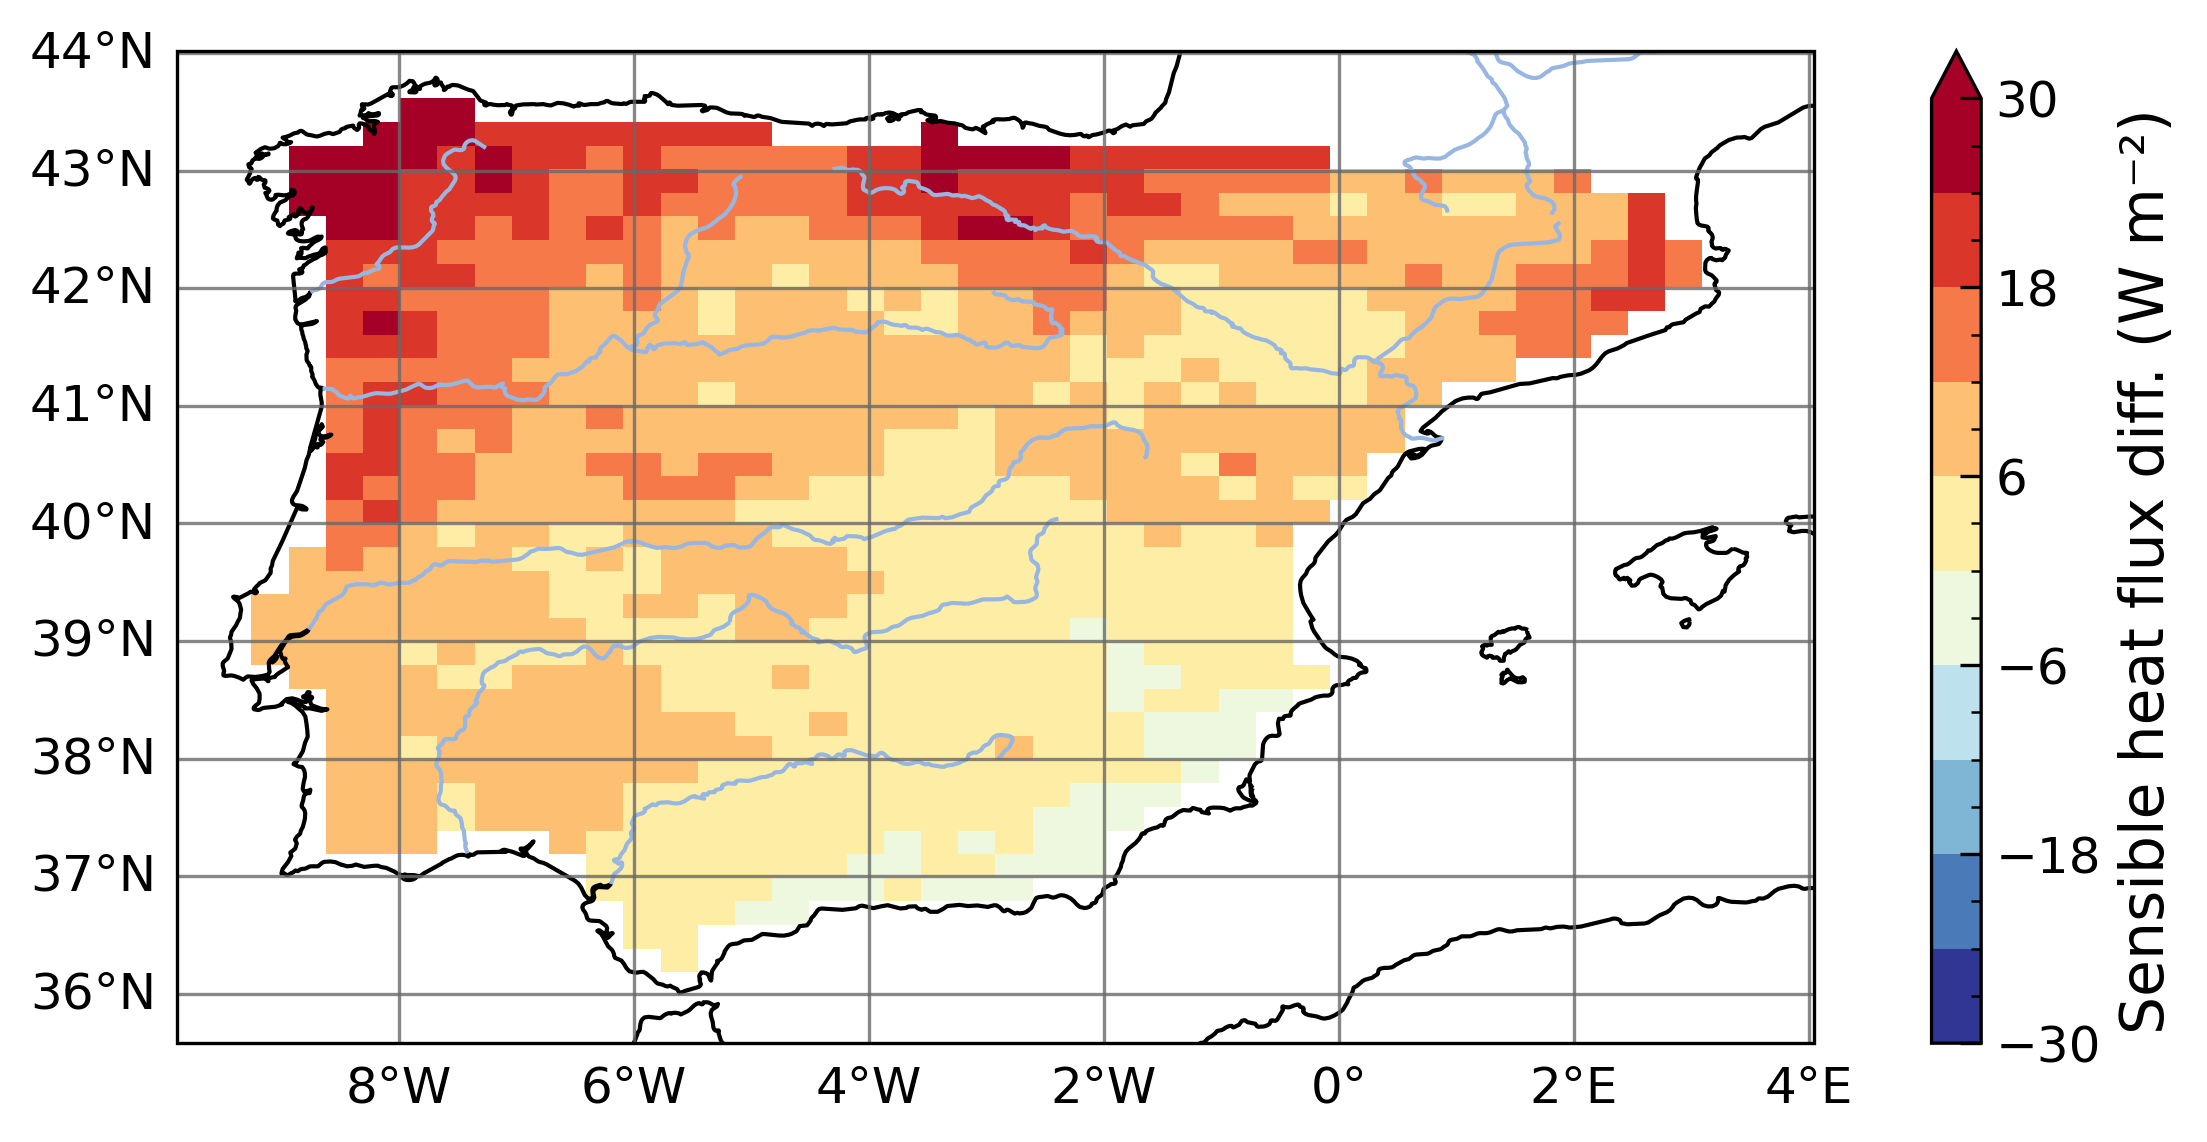
\includegraphics[width=\textwidth]{images/chap4/future/diffmap_JJA_fluxsens_presfut.png}
%         \end{subfigure} \\

%         %q2m
%         \begin{subfigure}[b]{0.5\textwidth}
%             \caption{}
%             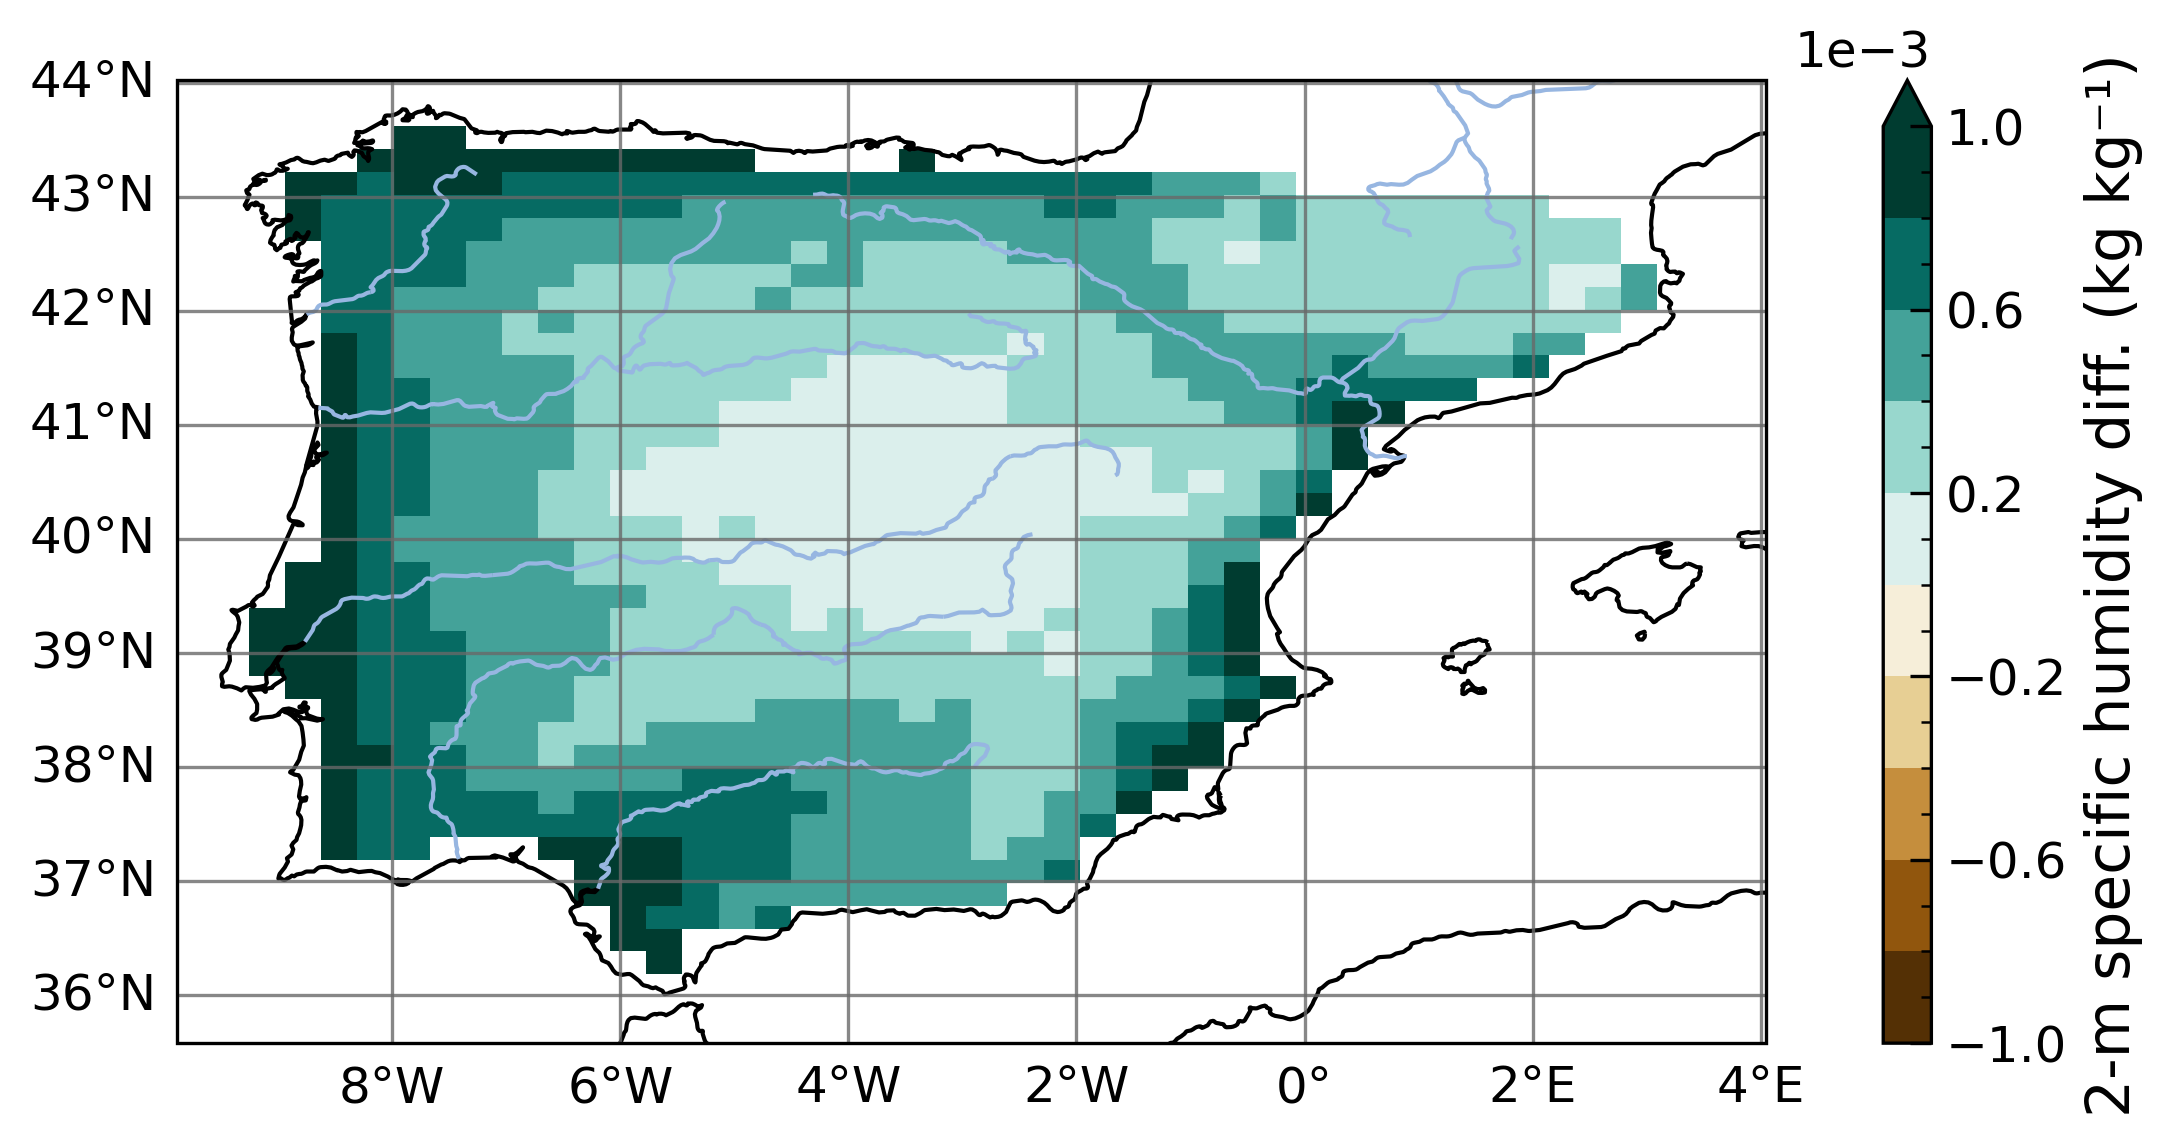
\includegraphics[width=\textwidth]{images/chap4/future/diffmap_JJA_q2m_presfut.png}
%         \end{subfigure} &
%         %rh2m
%         \begin{subfigure}[b]{0.5\textwidth}
%             \caption{}
%             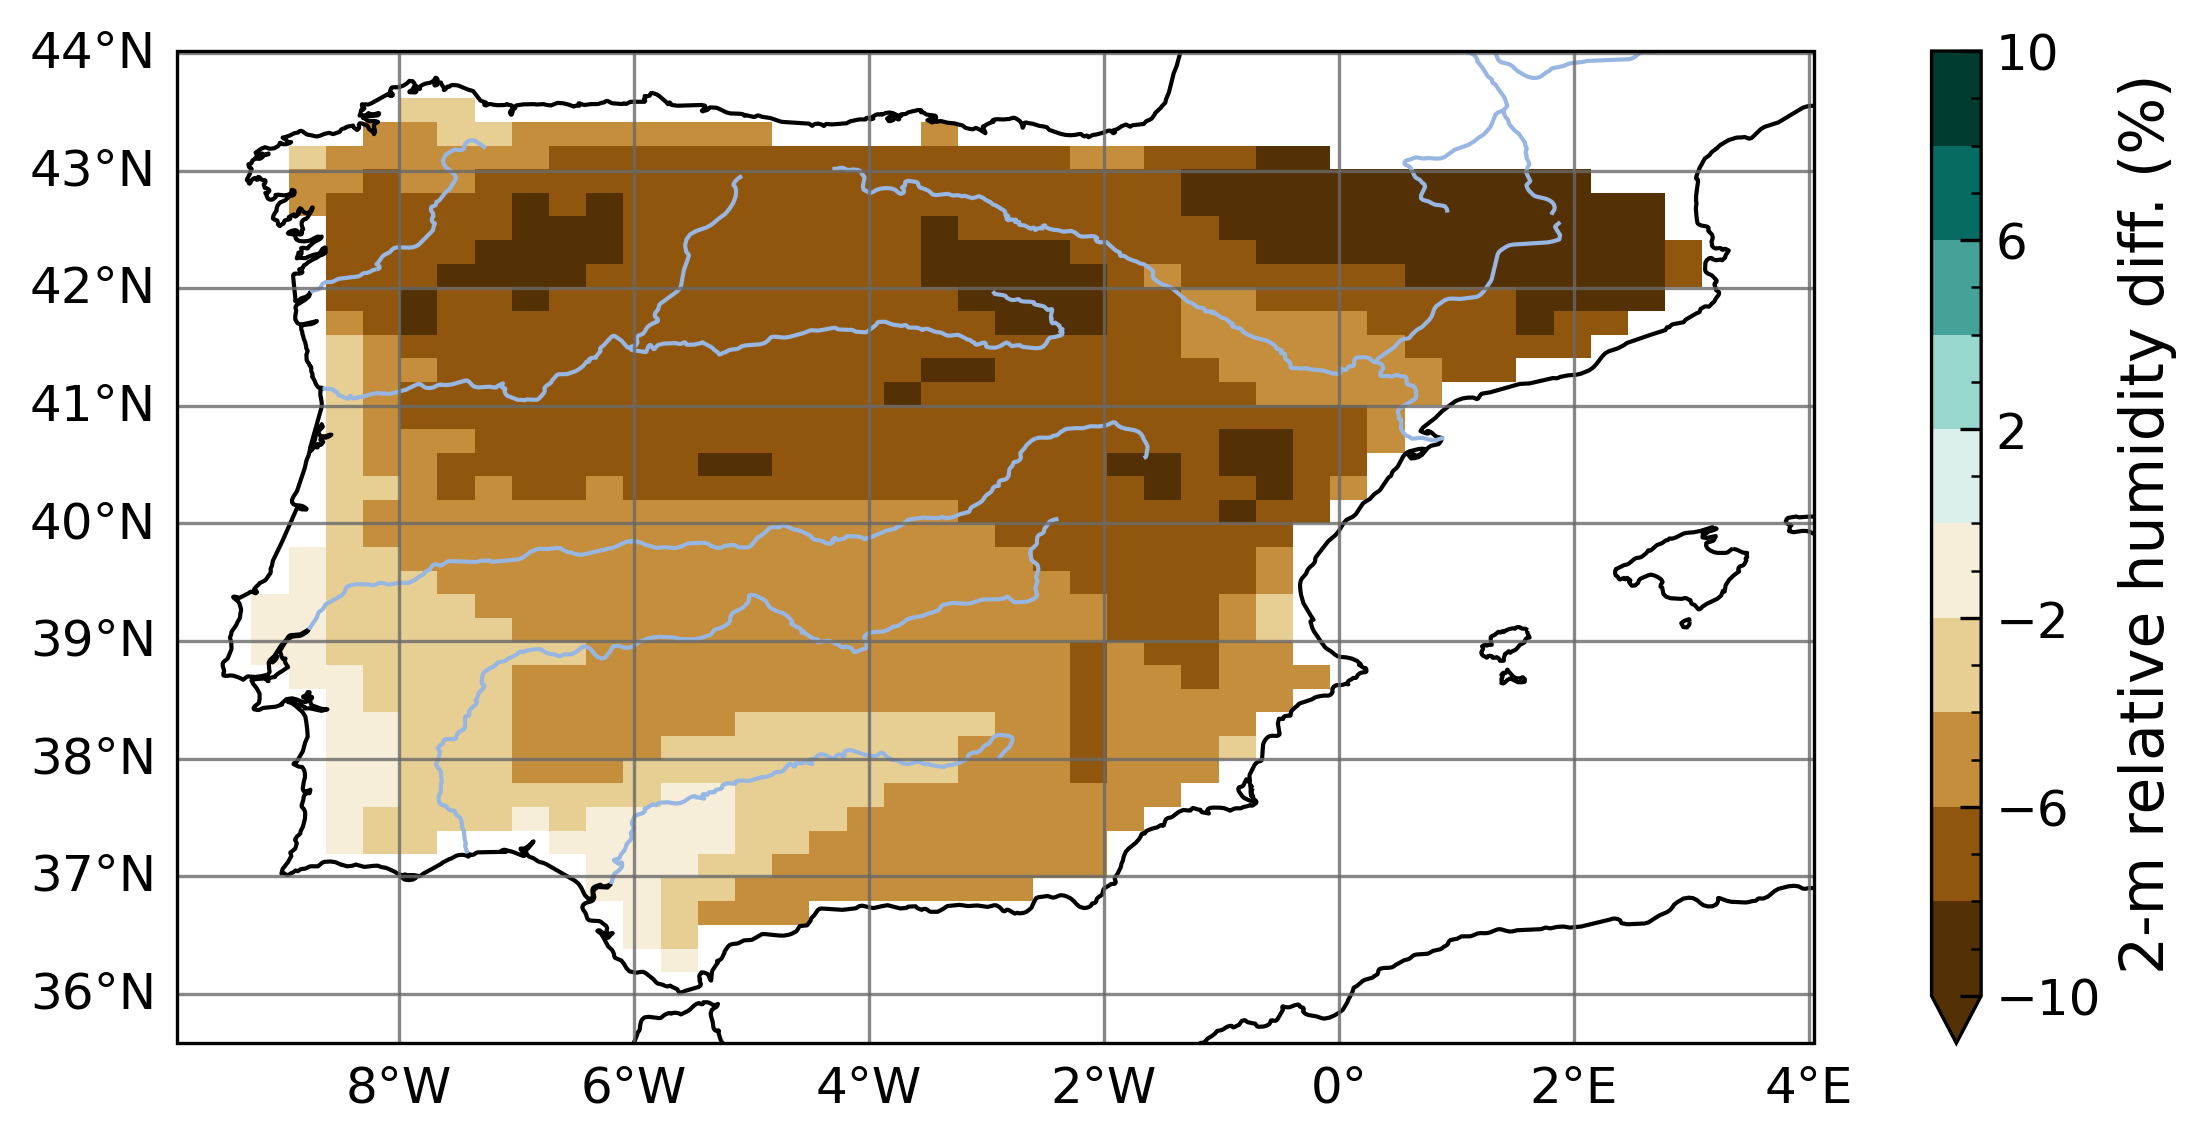
\includegraphics[width=\textwidth]{images/chap4/future/diffmap_JJA_rh2m_presfut.png}
%         \end{subfigure} \\

%         %pblh
%         \begin{subfigure}[b]{0.5\textwidth}
%             \caption{}
%             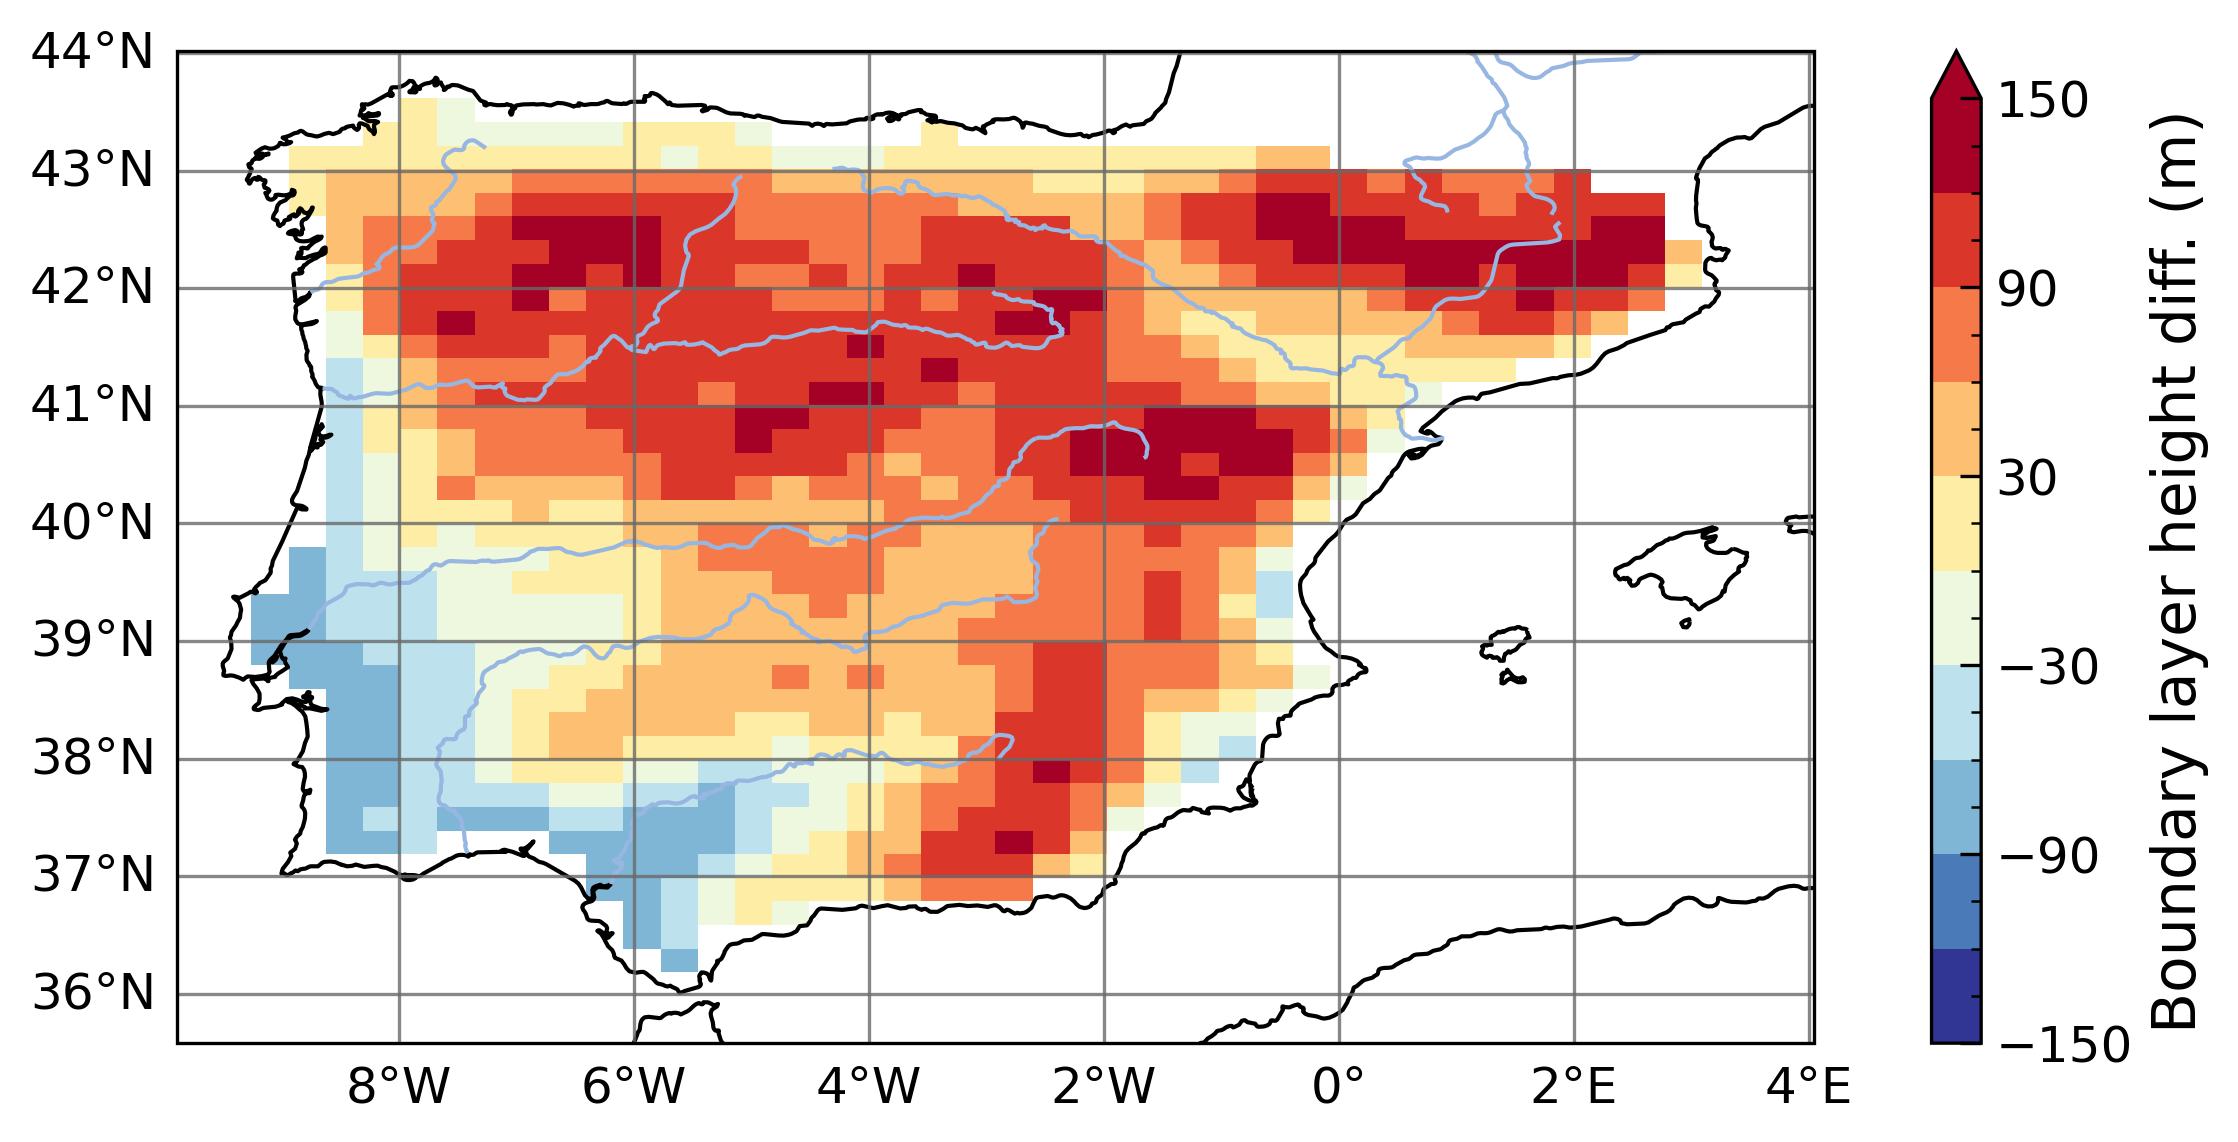
\includegraphics[width=\textwidth]{images/chap4/future/diffmap_JJA_s_pblh_presfut.png}
%         \end{subfigure} &
%         %lcl
%         \begin{subfigure}[b]{0.5\textwidth}
%             \caption{}
%             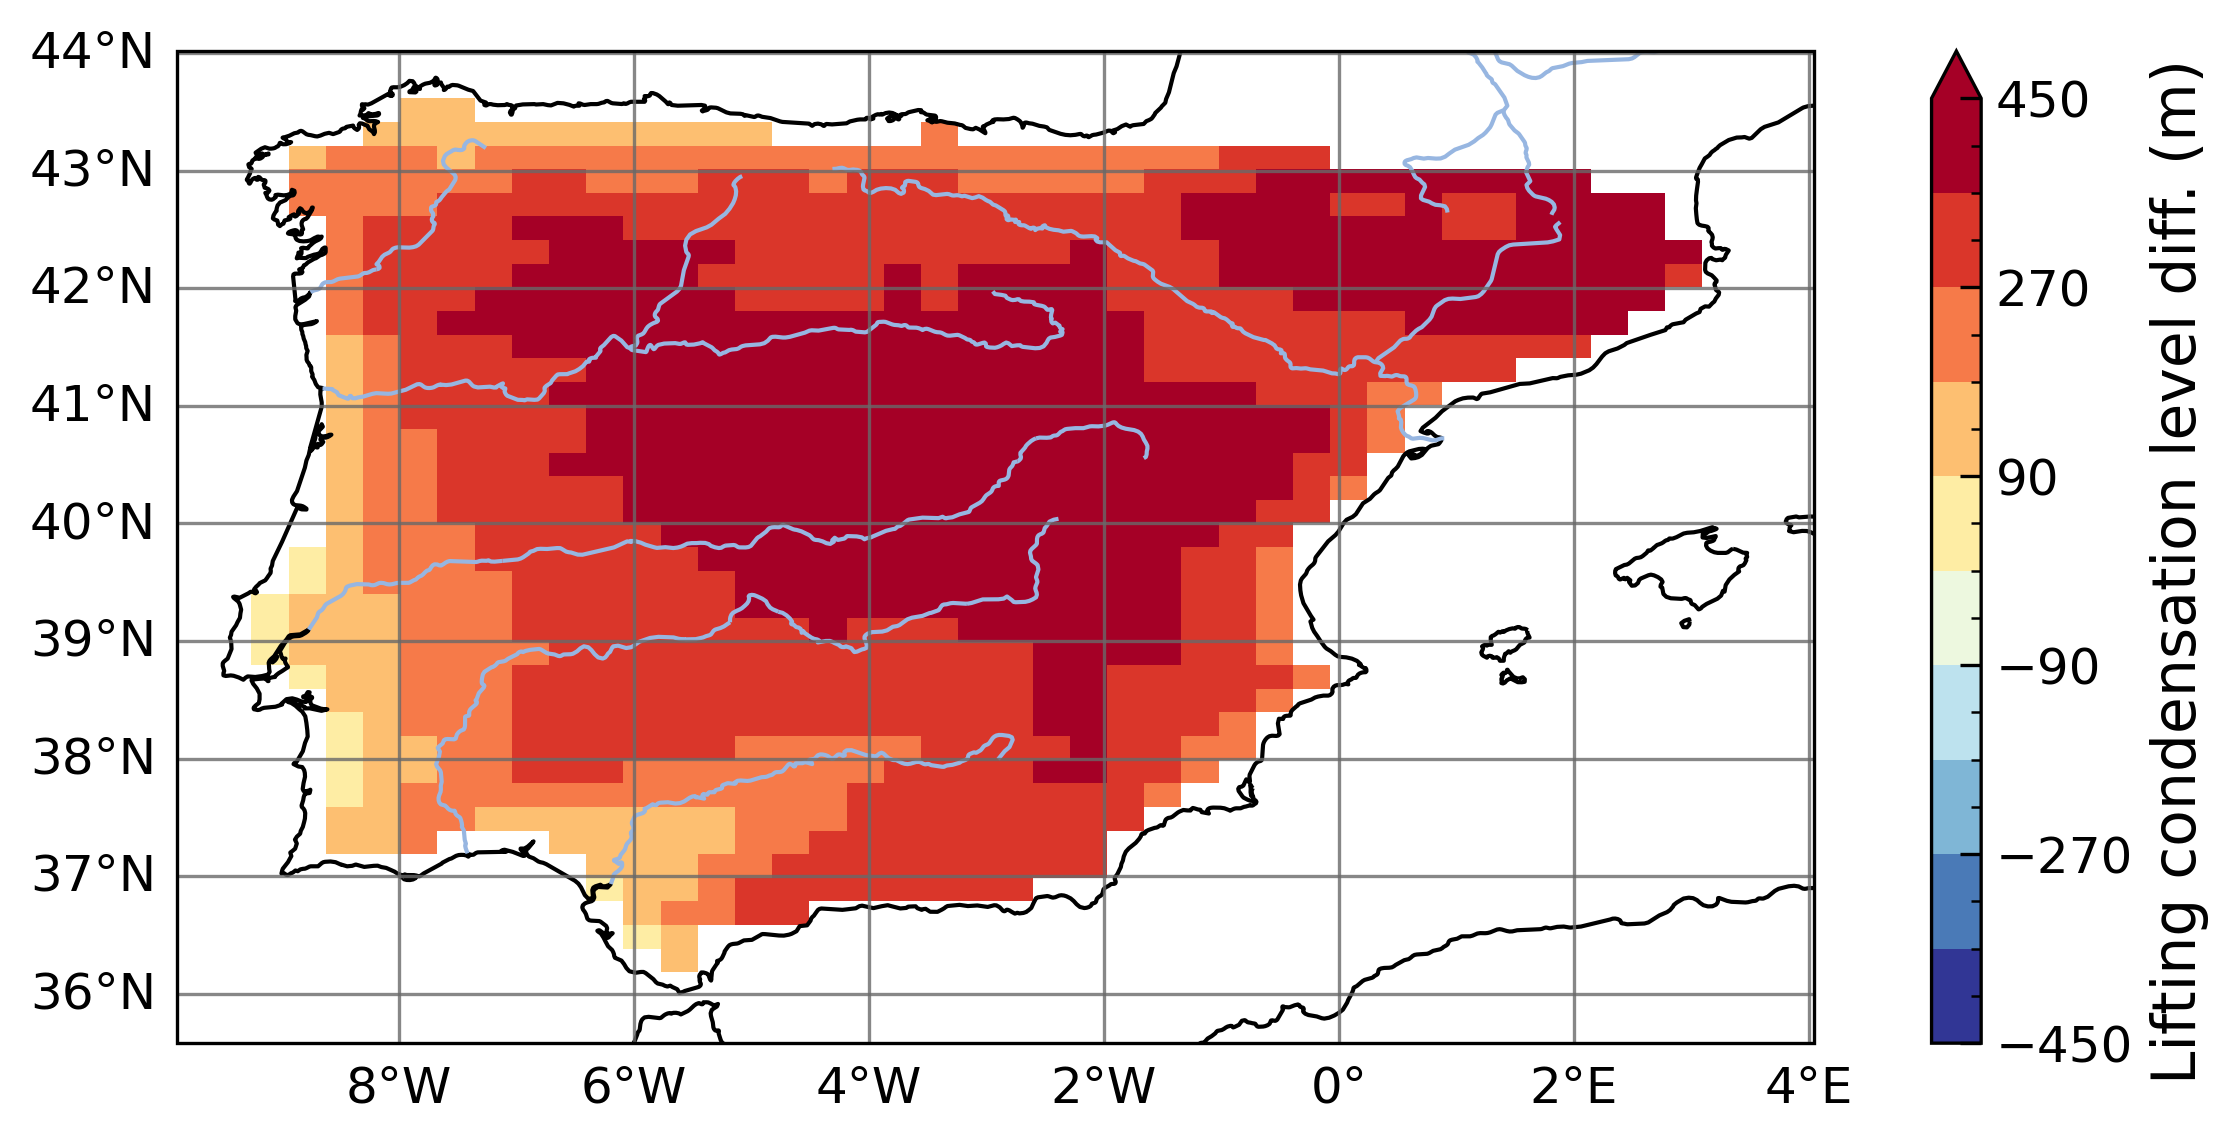
\includegraphics[width=\textwidth]{images/chap4/future/diffmap_JJA_s_lcl_presfut.png}
%         \end{subfigure} \\
%     \end{tabular}
%     \caption{JJA difference (\futnoirr - \presnoirr)}
%     \label{fig:diffmaps_JJA_present_future}
% \end{figure}

%figure : relative diff maps annual (noirr, pres - future)
\begin{figure}[htbp]
    \centering
    \begin{tabular}{cc}
        %precip
        \begin{subfigure}[b]{0.5\textwidth}
            \caption{}
            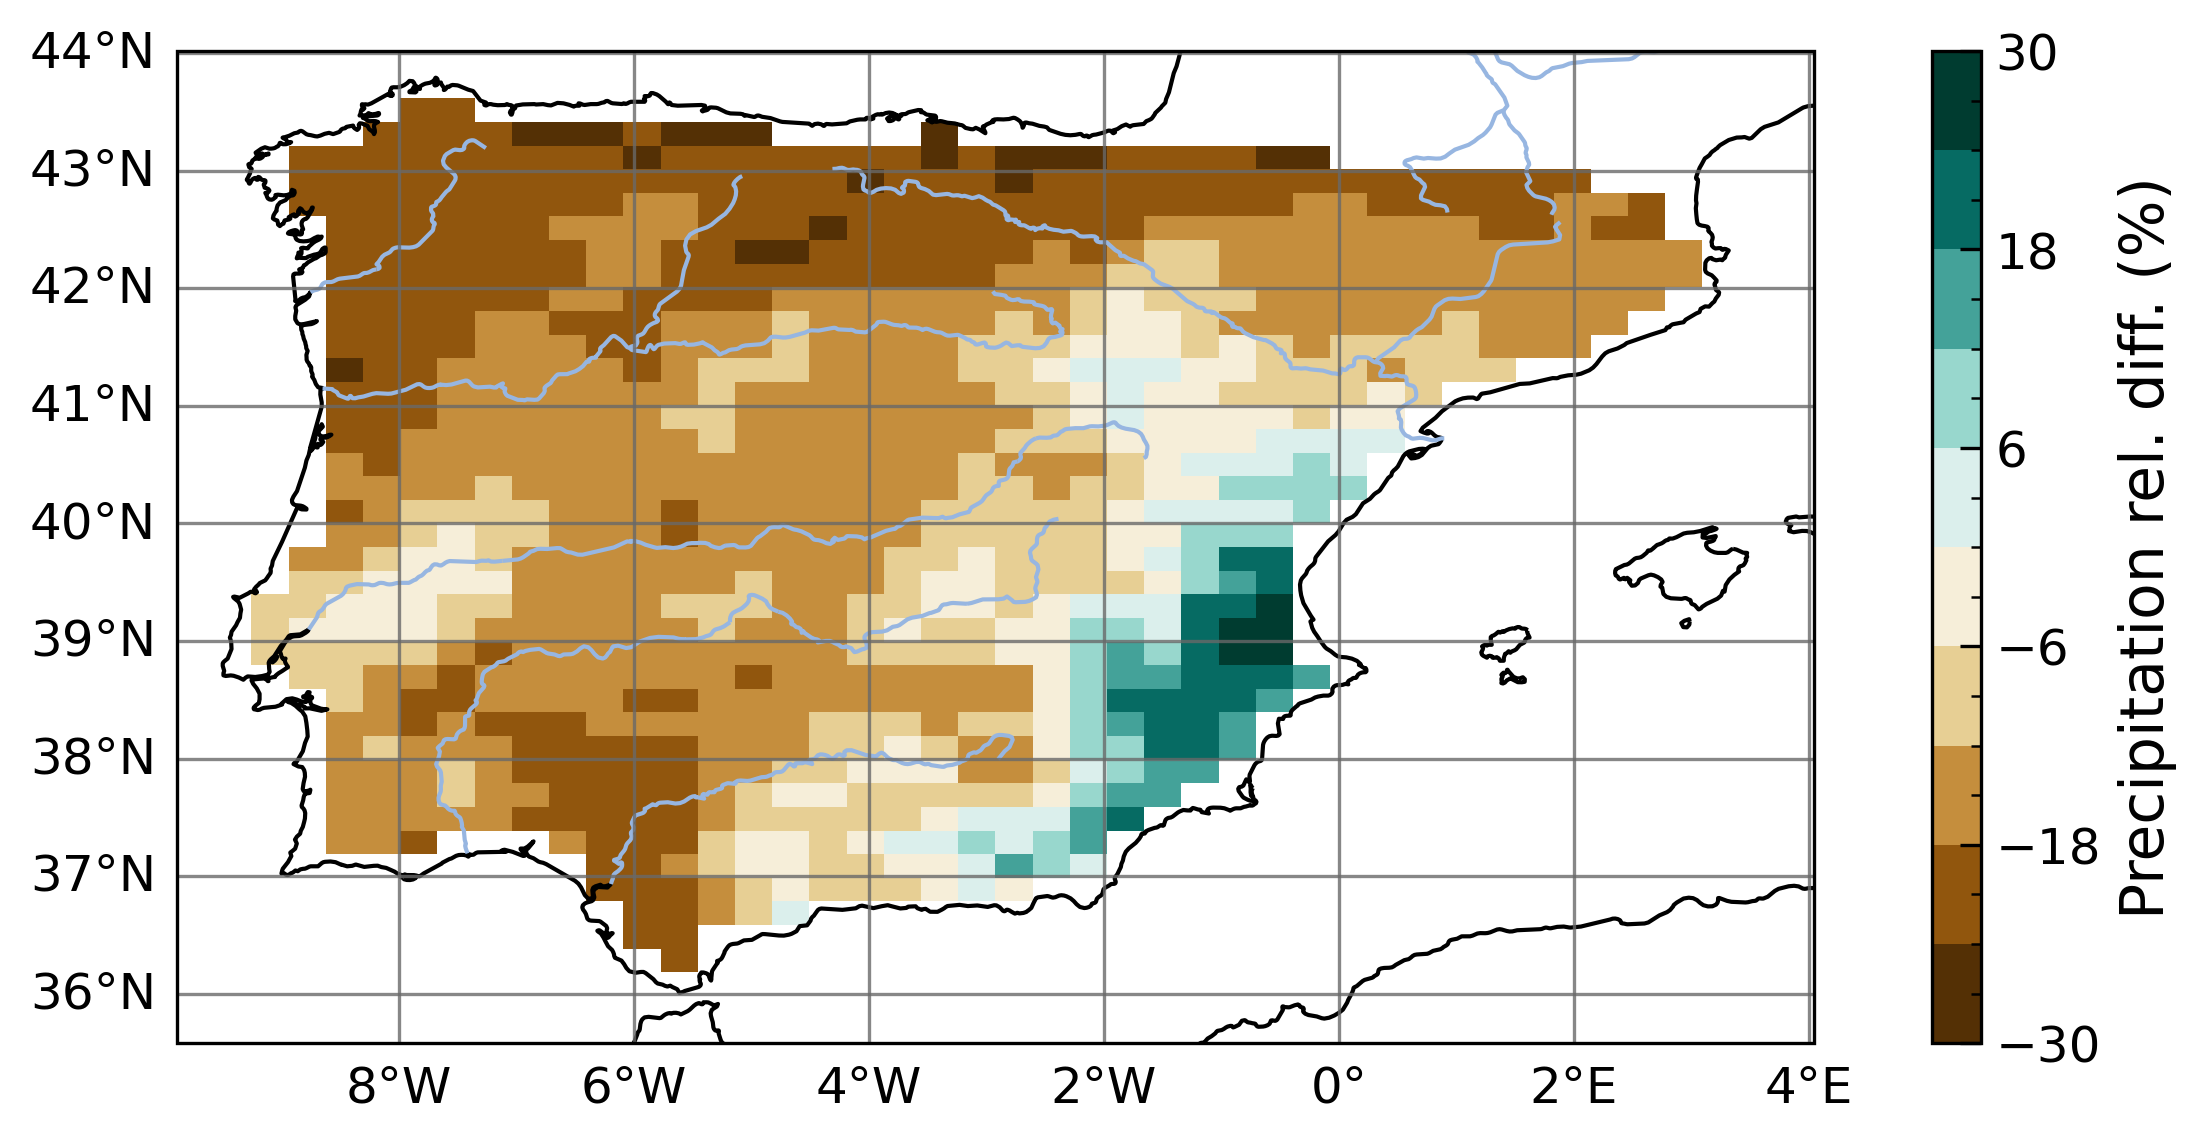
\includegraphics[width=\textwidth]{images/chap4/future/reldiffmap_precip_presfut.png}
        \end{subfigure} &
        %evap
        \begin{subfigure}[b]{0.5\textwidth}
            \caption{}
            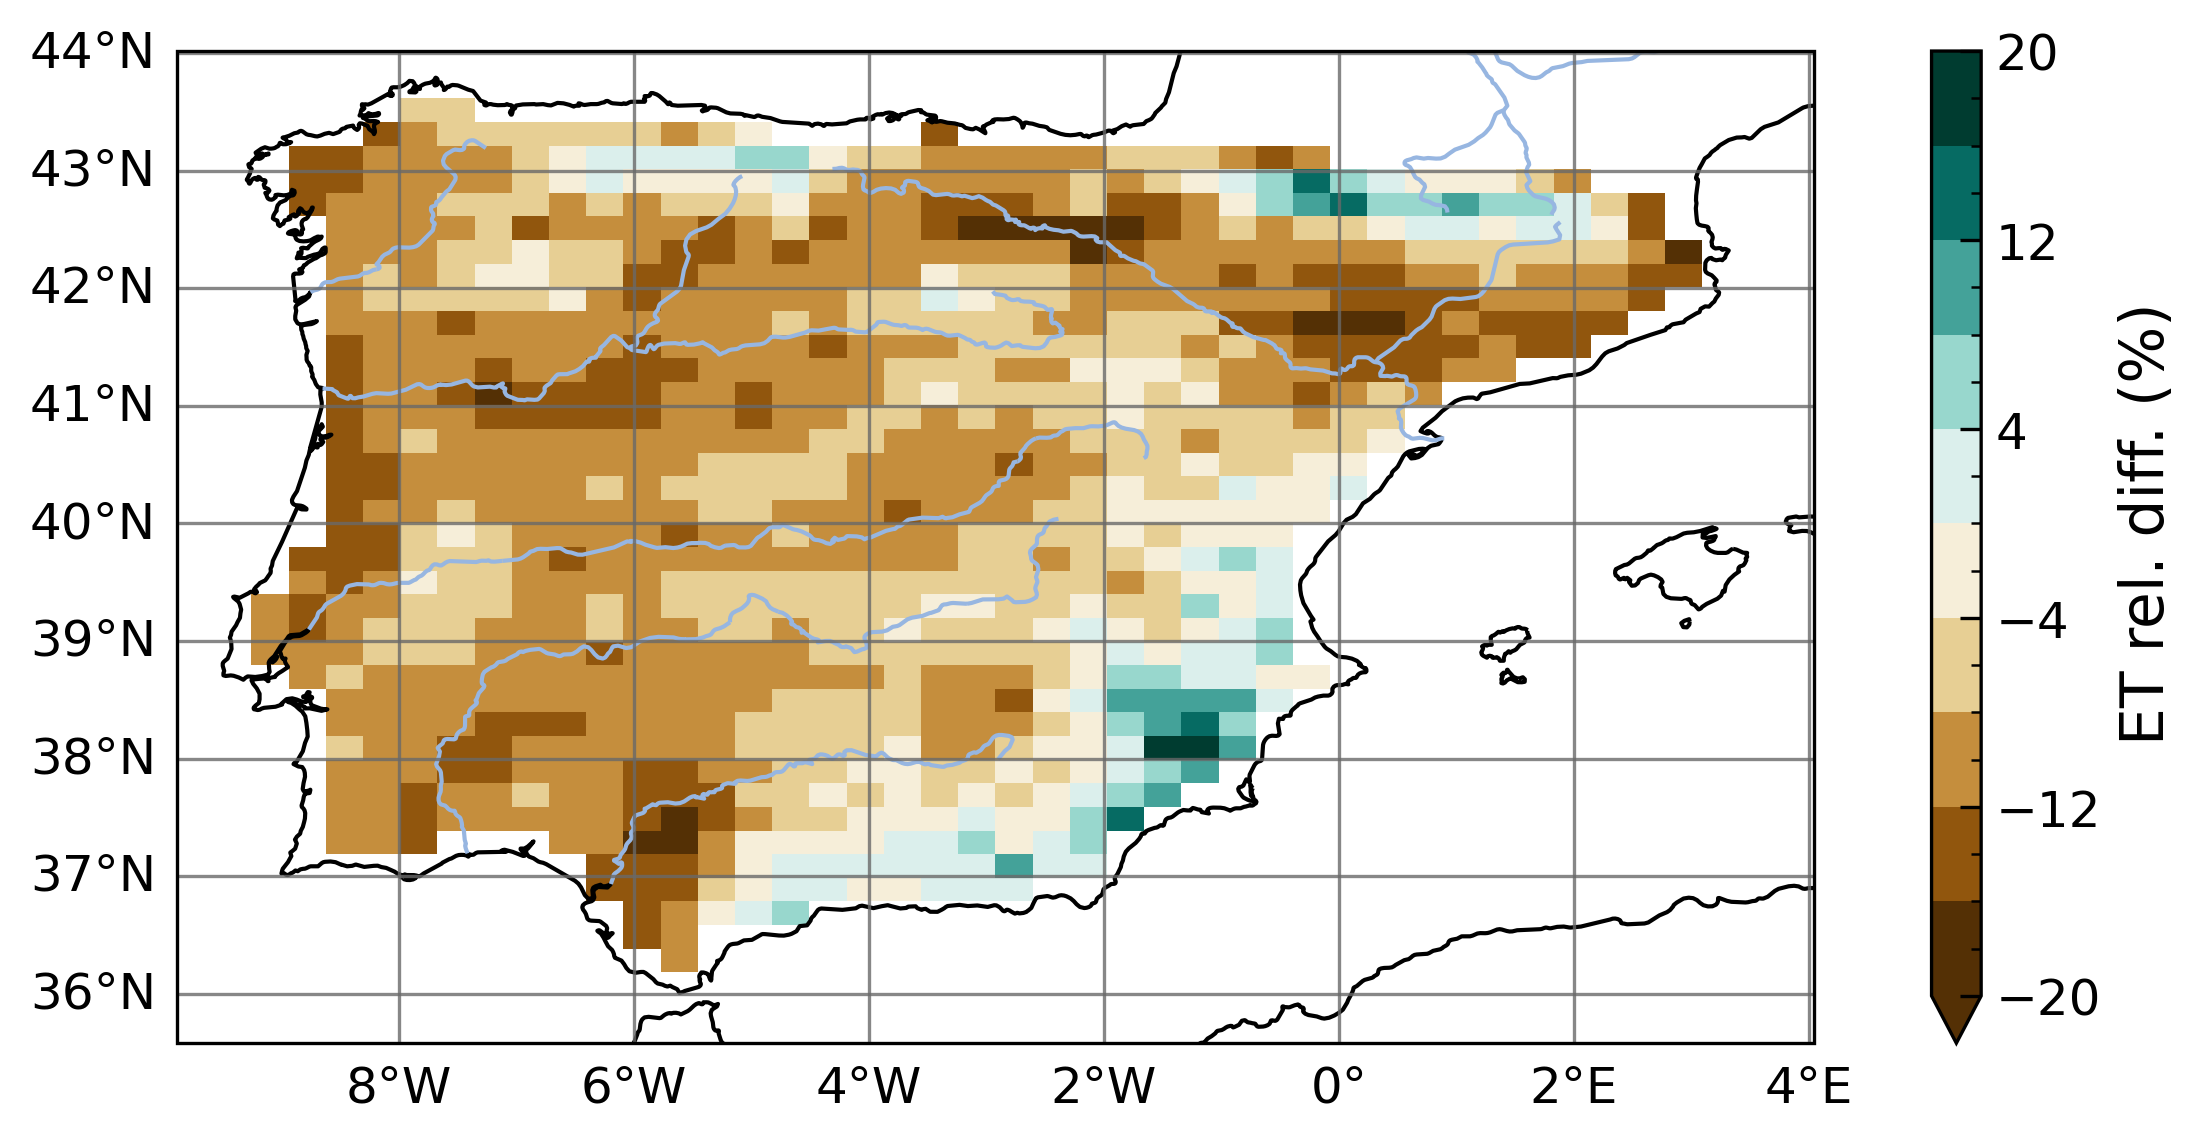
\includegraphics[width=\textwidth]{images/chap4/future/reldiffmap_evap_presfut.png}
        \end{subfigure} \\

        %t2m
        \begin{subfigure}[b]{0.5\textwidth}
            \caption{}
            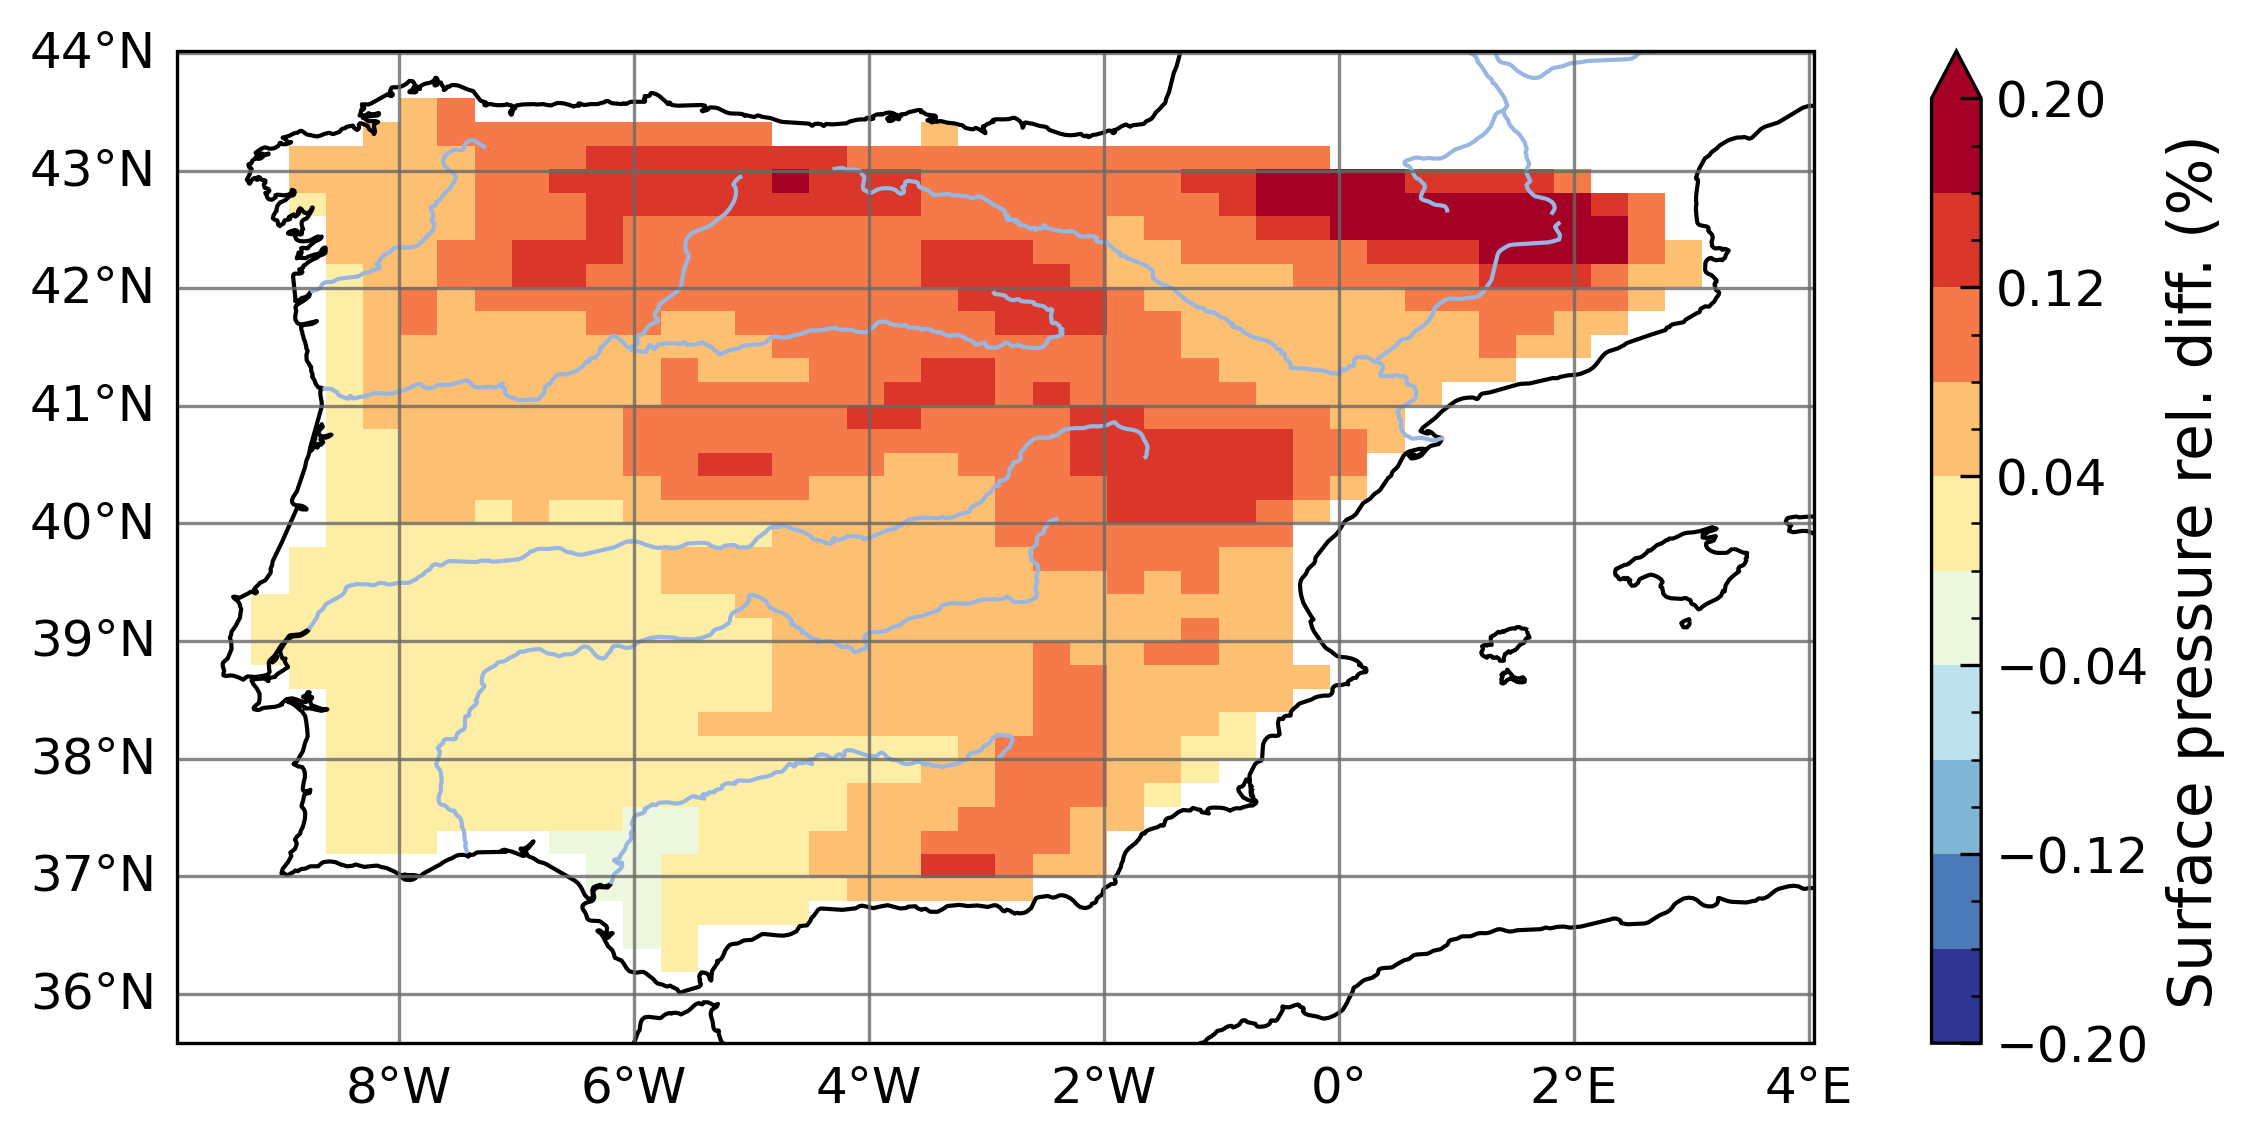
\includegraphics[width=\textwidth]{images/chap4/future/reldiffmap_psol_presfut.png}
        \end{subfigure} &
        %fluxsens
        \begin{subfigure}[b]{0.5\textwidth}
            \caption{}
            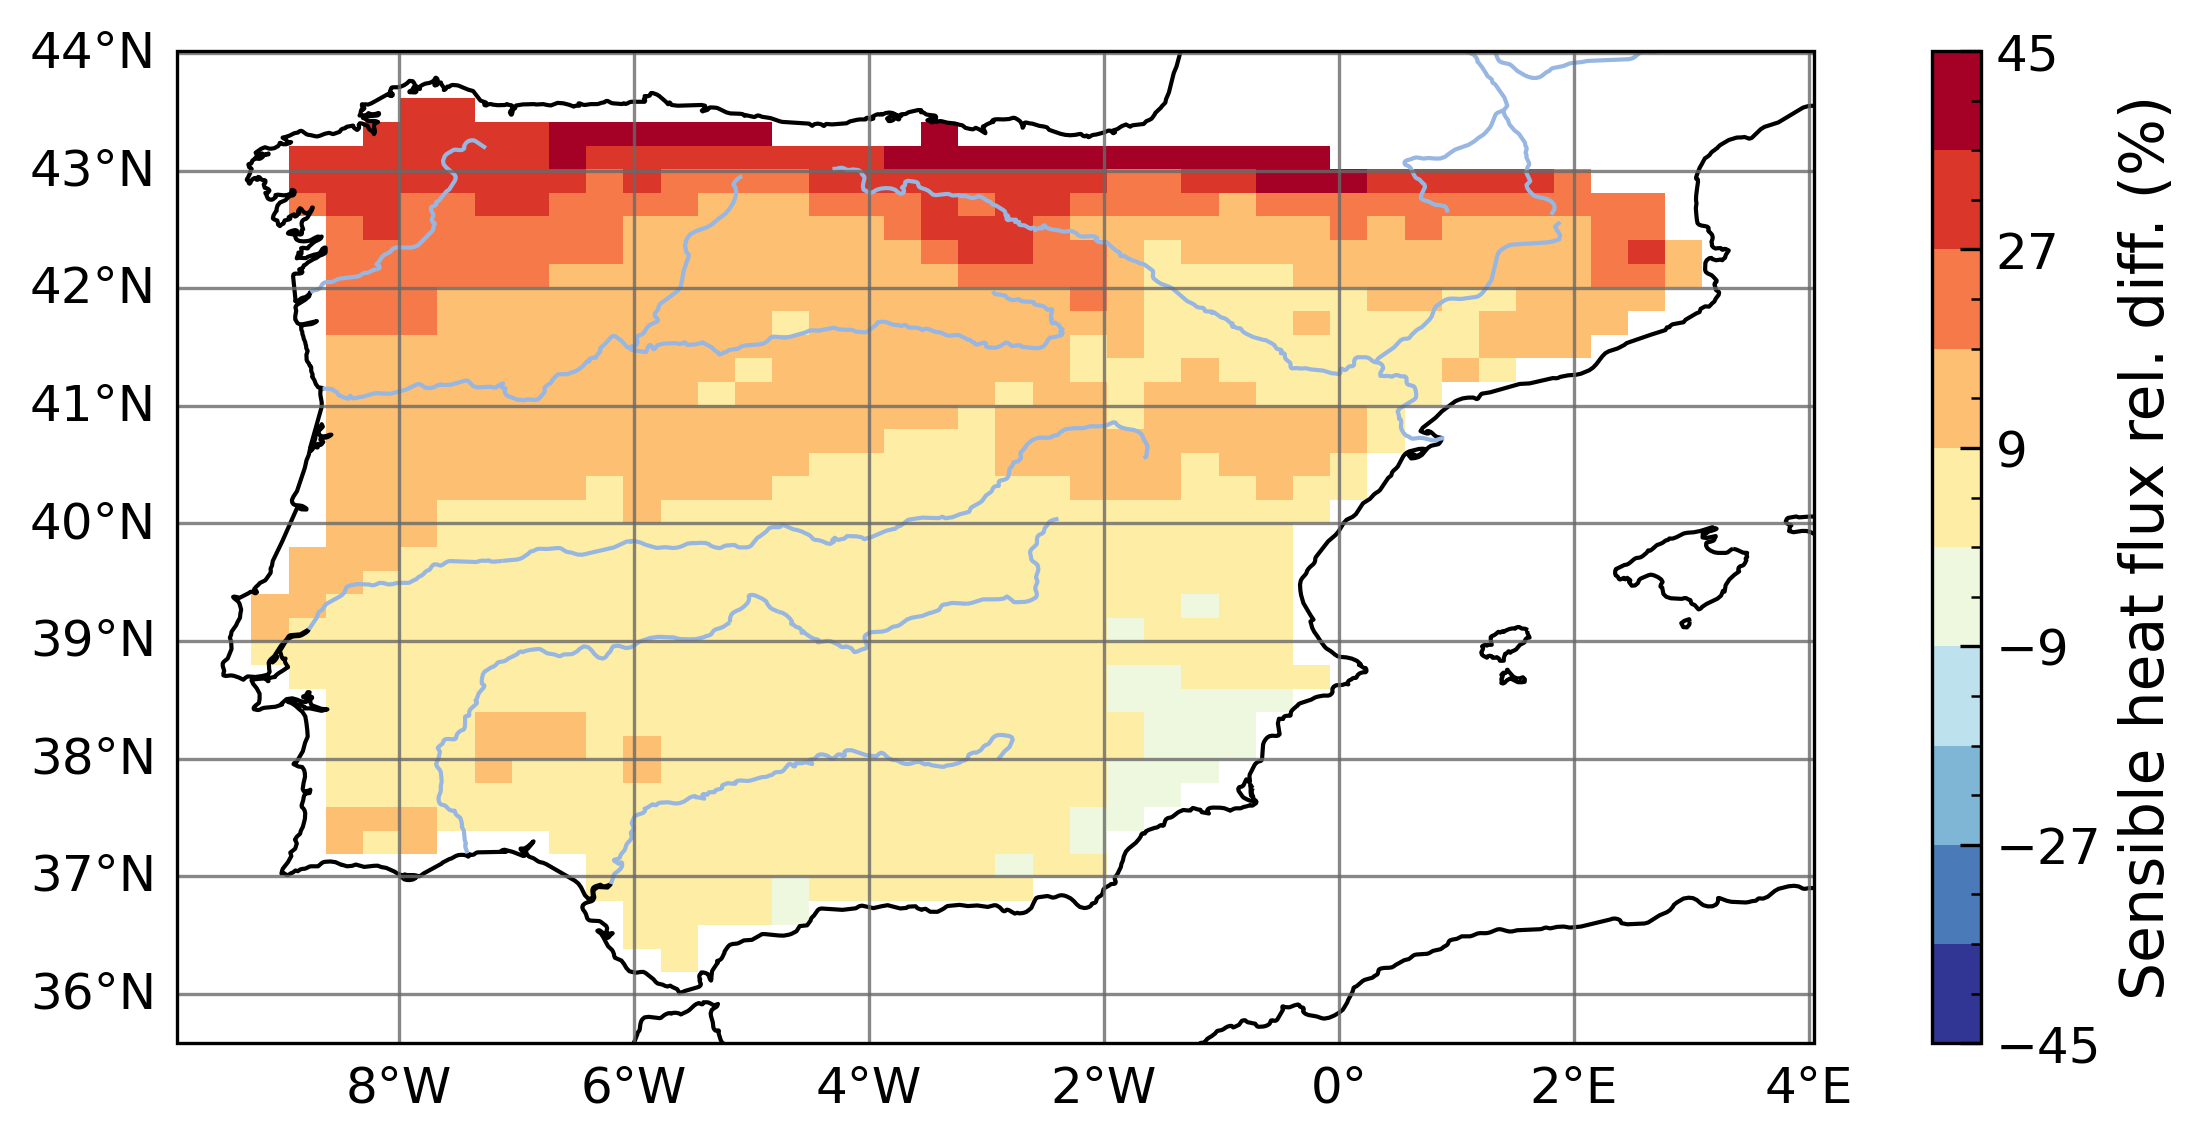
\includegraphics[width=\textwidth]{images/chap4/future/reldiffmap_fluxsens_presfut.png}
        \end{subfigure} \\

        %q2m
        \begin{subfigure}[b]{0.5\textwidth}
            \caption{}
            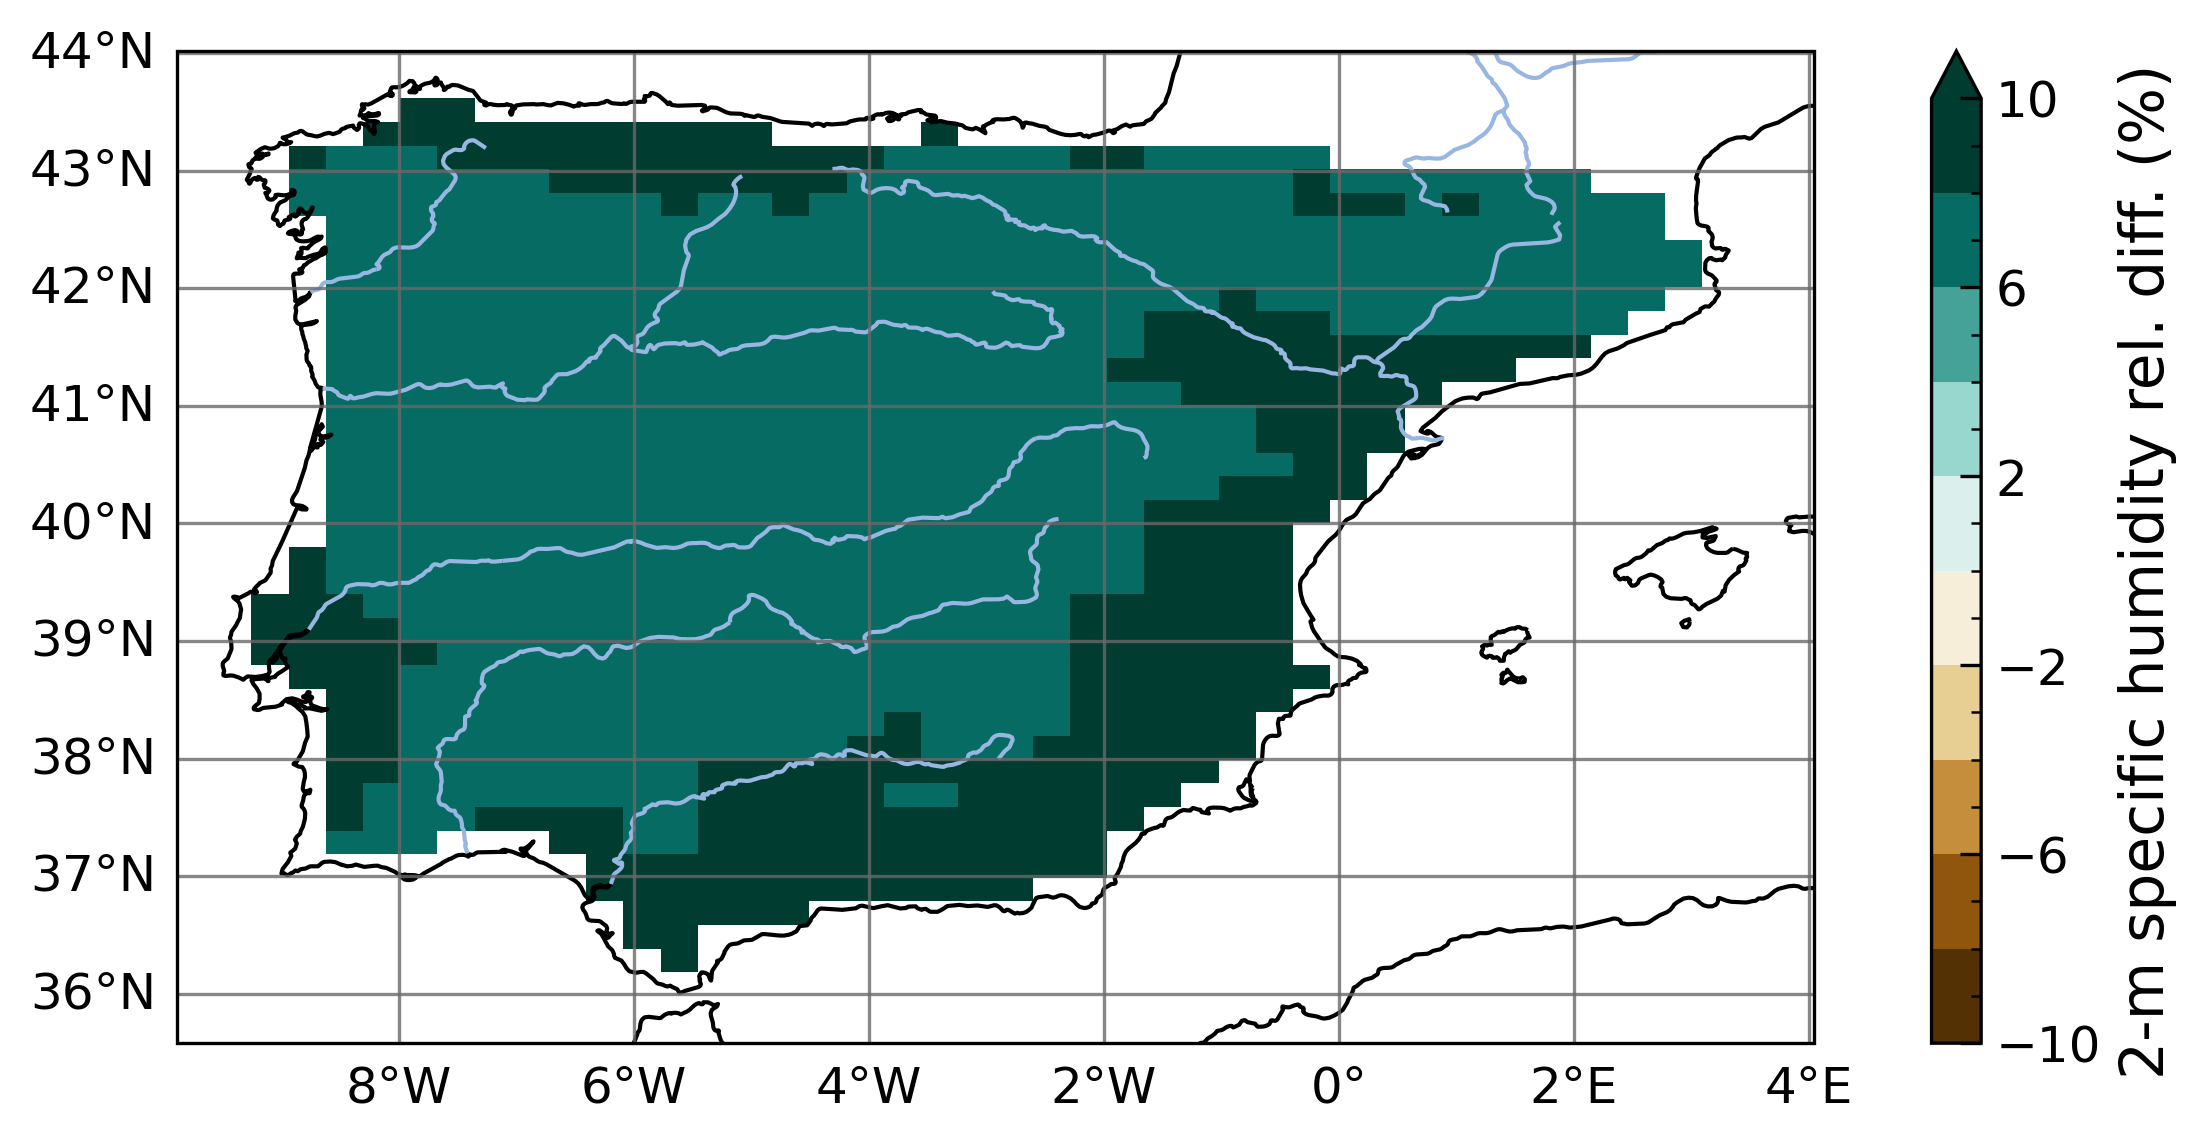
\includegraphics[width=\textwidth]{images/chap4/future/reldiffmap_q2m_presfut.png}
        \end{subfigure} &
        %rh2m
        \begin{subfigure}[b]{0.5\textwidth}
            \caption{}
            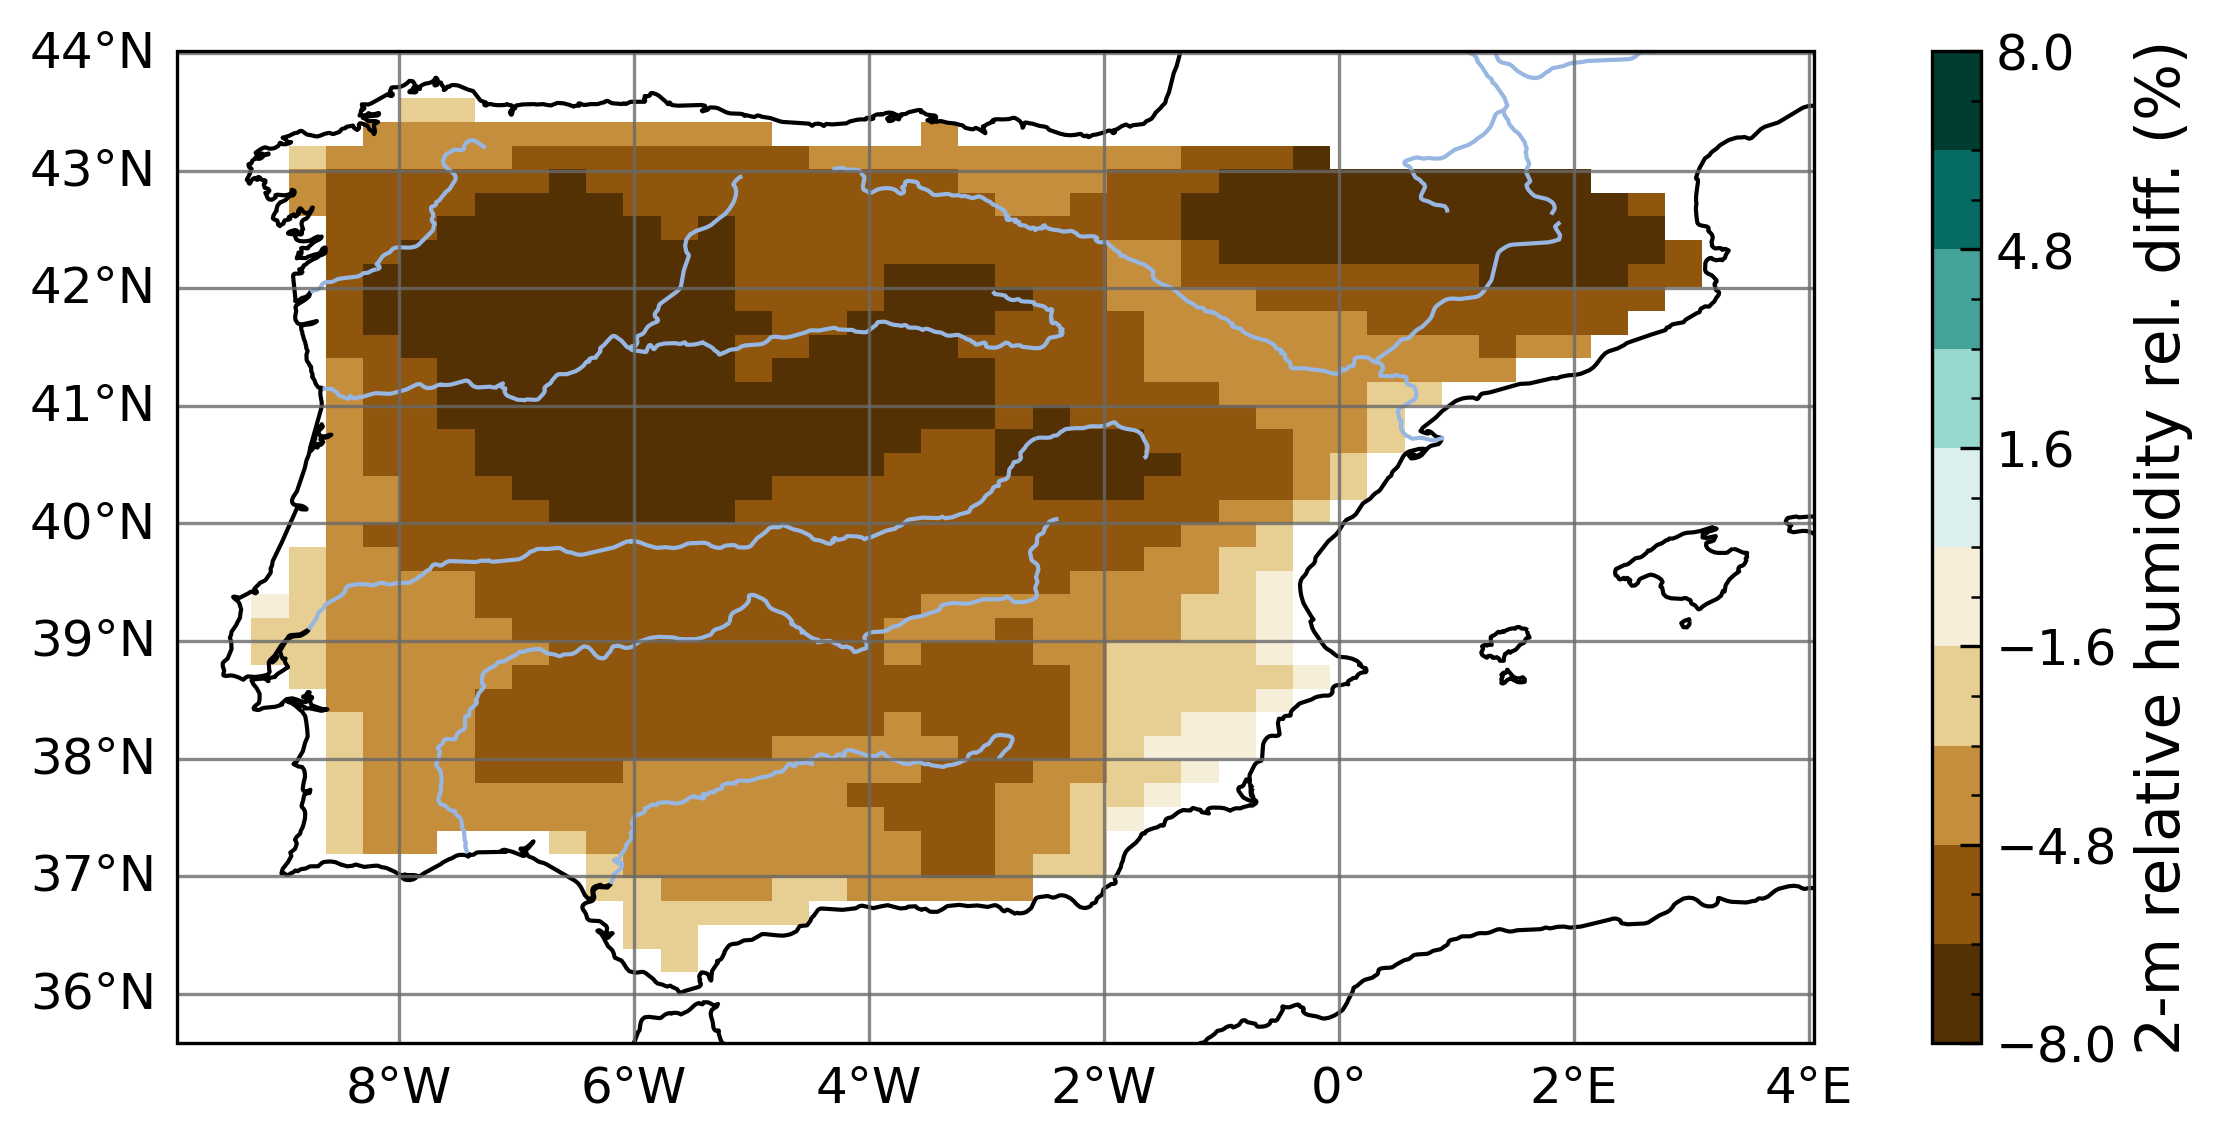
\includegraphics[width=\textwidth]{images/chap4/future/reldiffmap_rh2m_presfut.png}
        \end{subfigure} \\

        %pblh
        \begin{subfigure}[b]{0.5\textwidth}
            \caption{}
            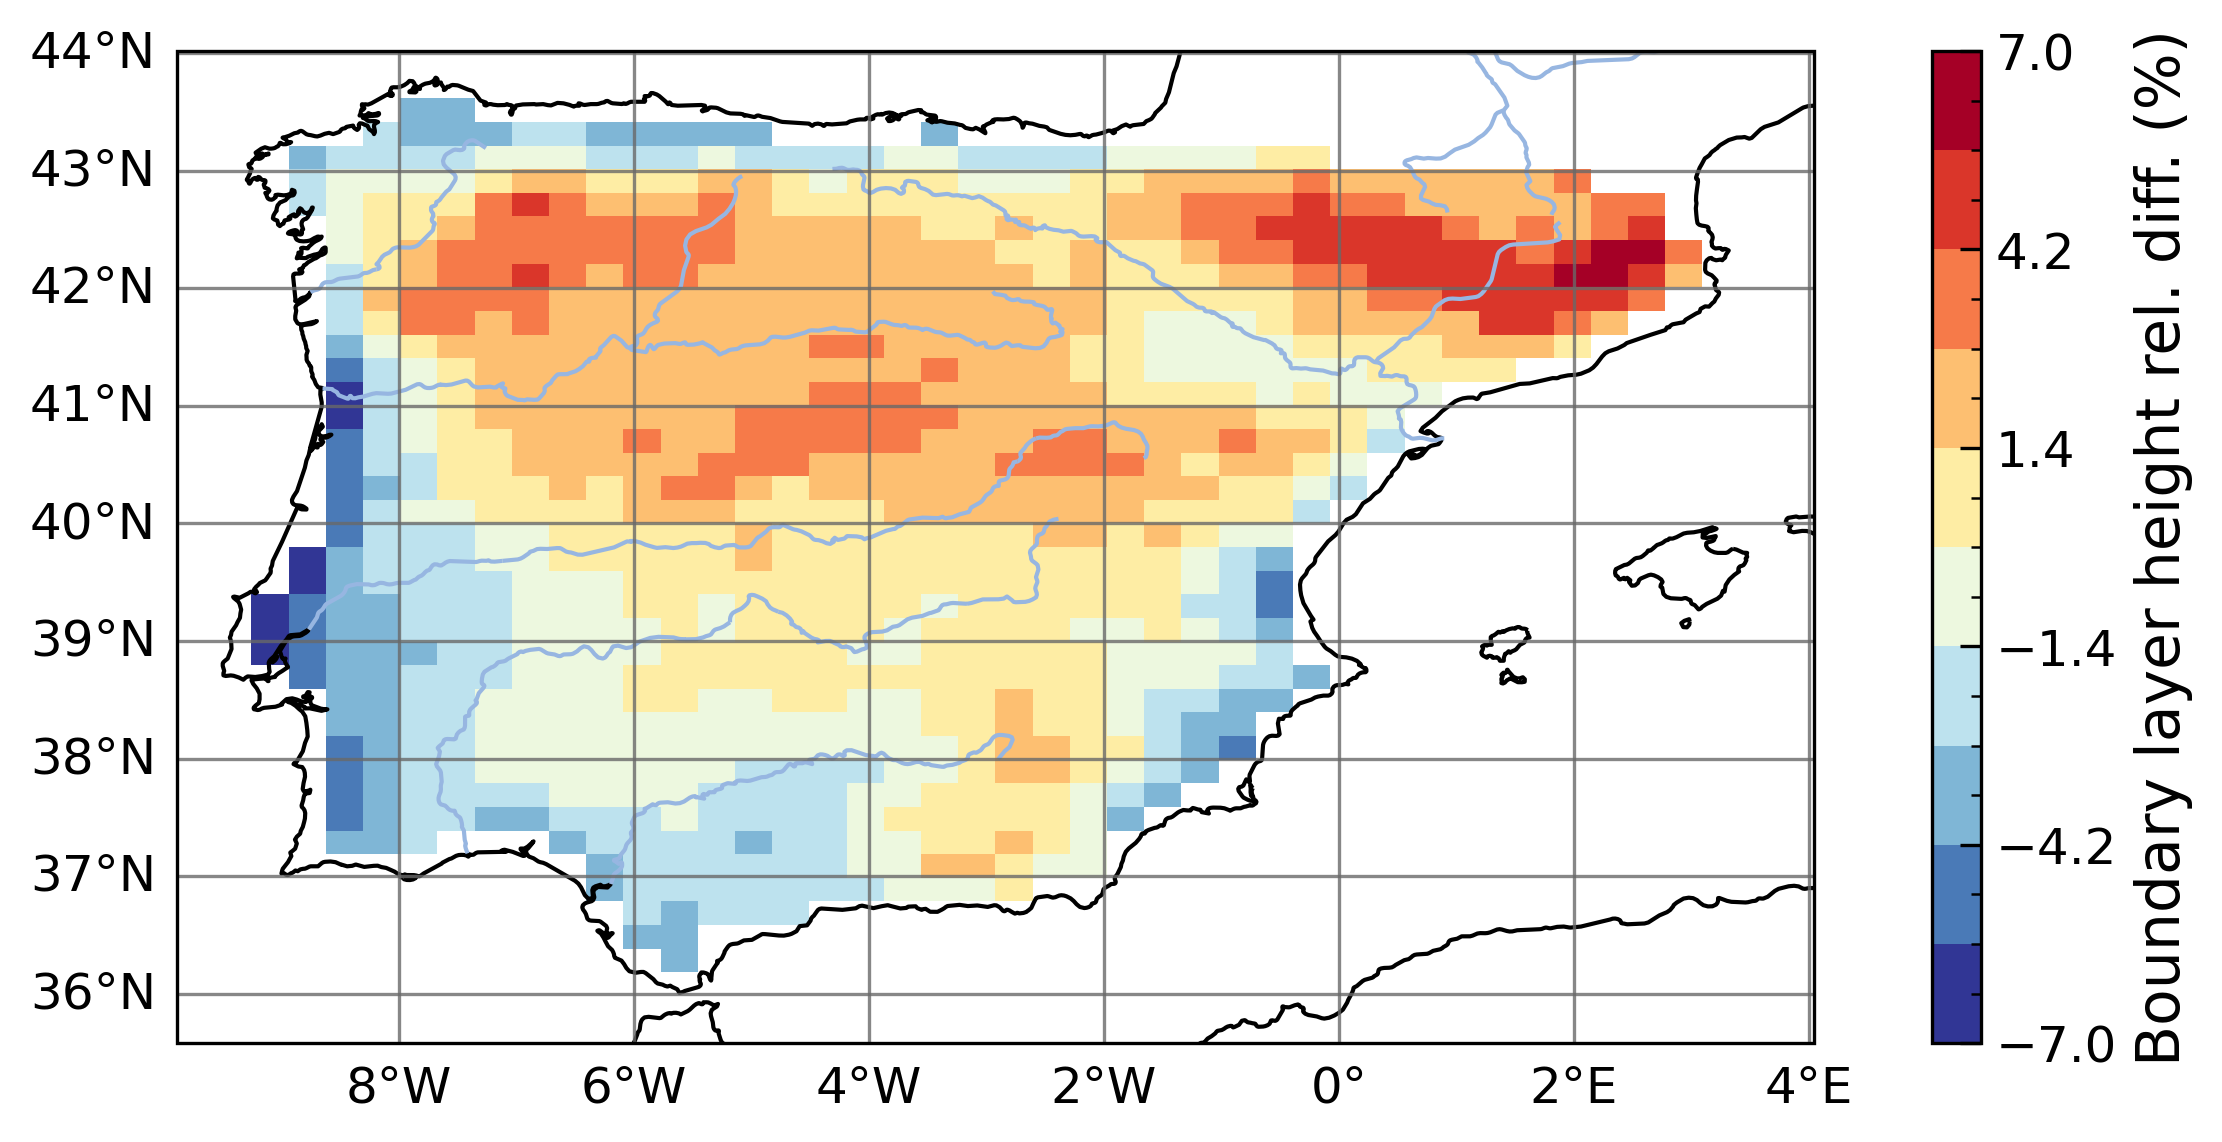
\includegraphics[width=\textwidth]{images/chap4/future/reldiffmap_s_pblh_presfut.png}
        \end{subfigure} &
        %lcl
        \begin{subfigure}[b]{0.5\textwidth}
            \caption{}
            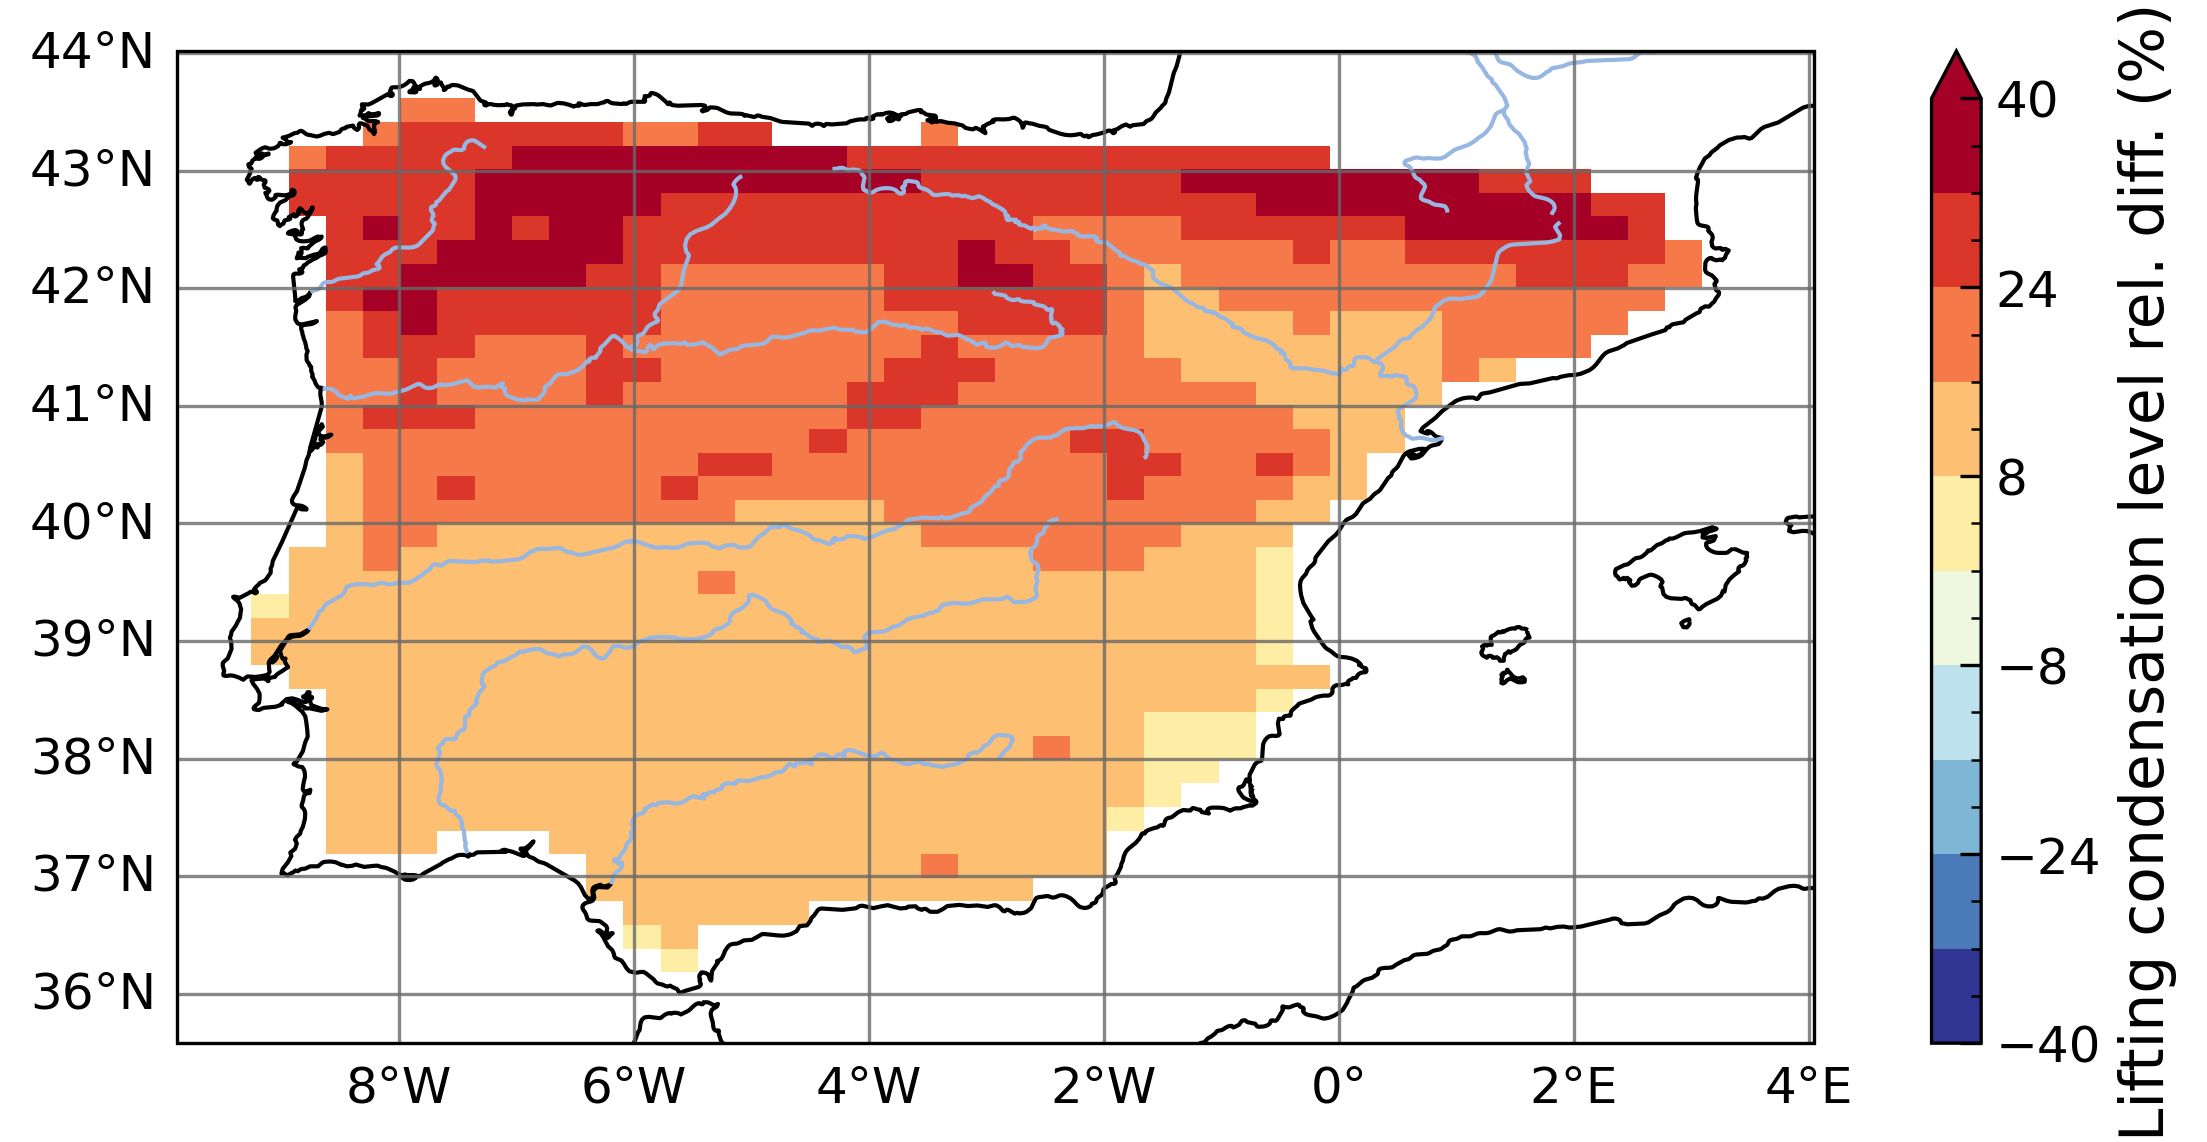
\includegraphics[width=\textwidth]{images/chap4/future/reldiffmap_s_lcl_presfut.png}
        \end{subfigure} \\
    \end{tabular}
    \caption{Relative difference, \futnoirr - \presnoirr}
    \label{fig:reldiffmaps_present_future}
\end{figure}

%figure : diff maps JJA (future, irr - no_irr)
% \begin{figure}[htbp]
%     \centering
%     \begin{tabular}{cc}
%         %precip
%         \begin{subfigure}[b]{0.5\textwidth}
%             \caption{}
%             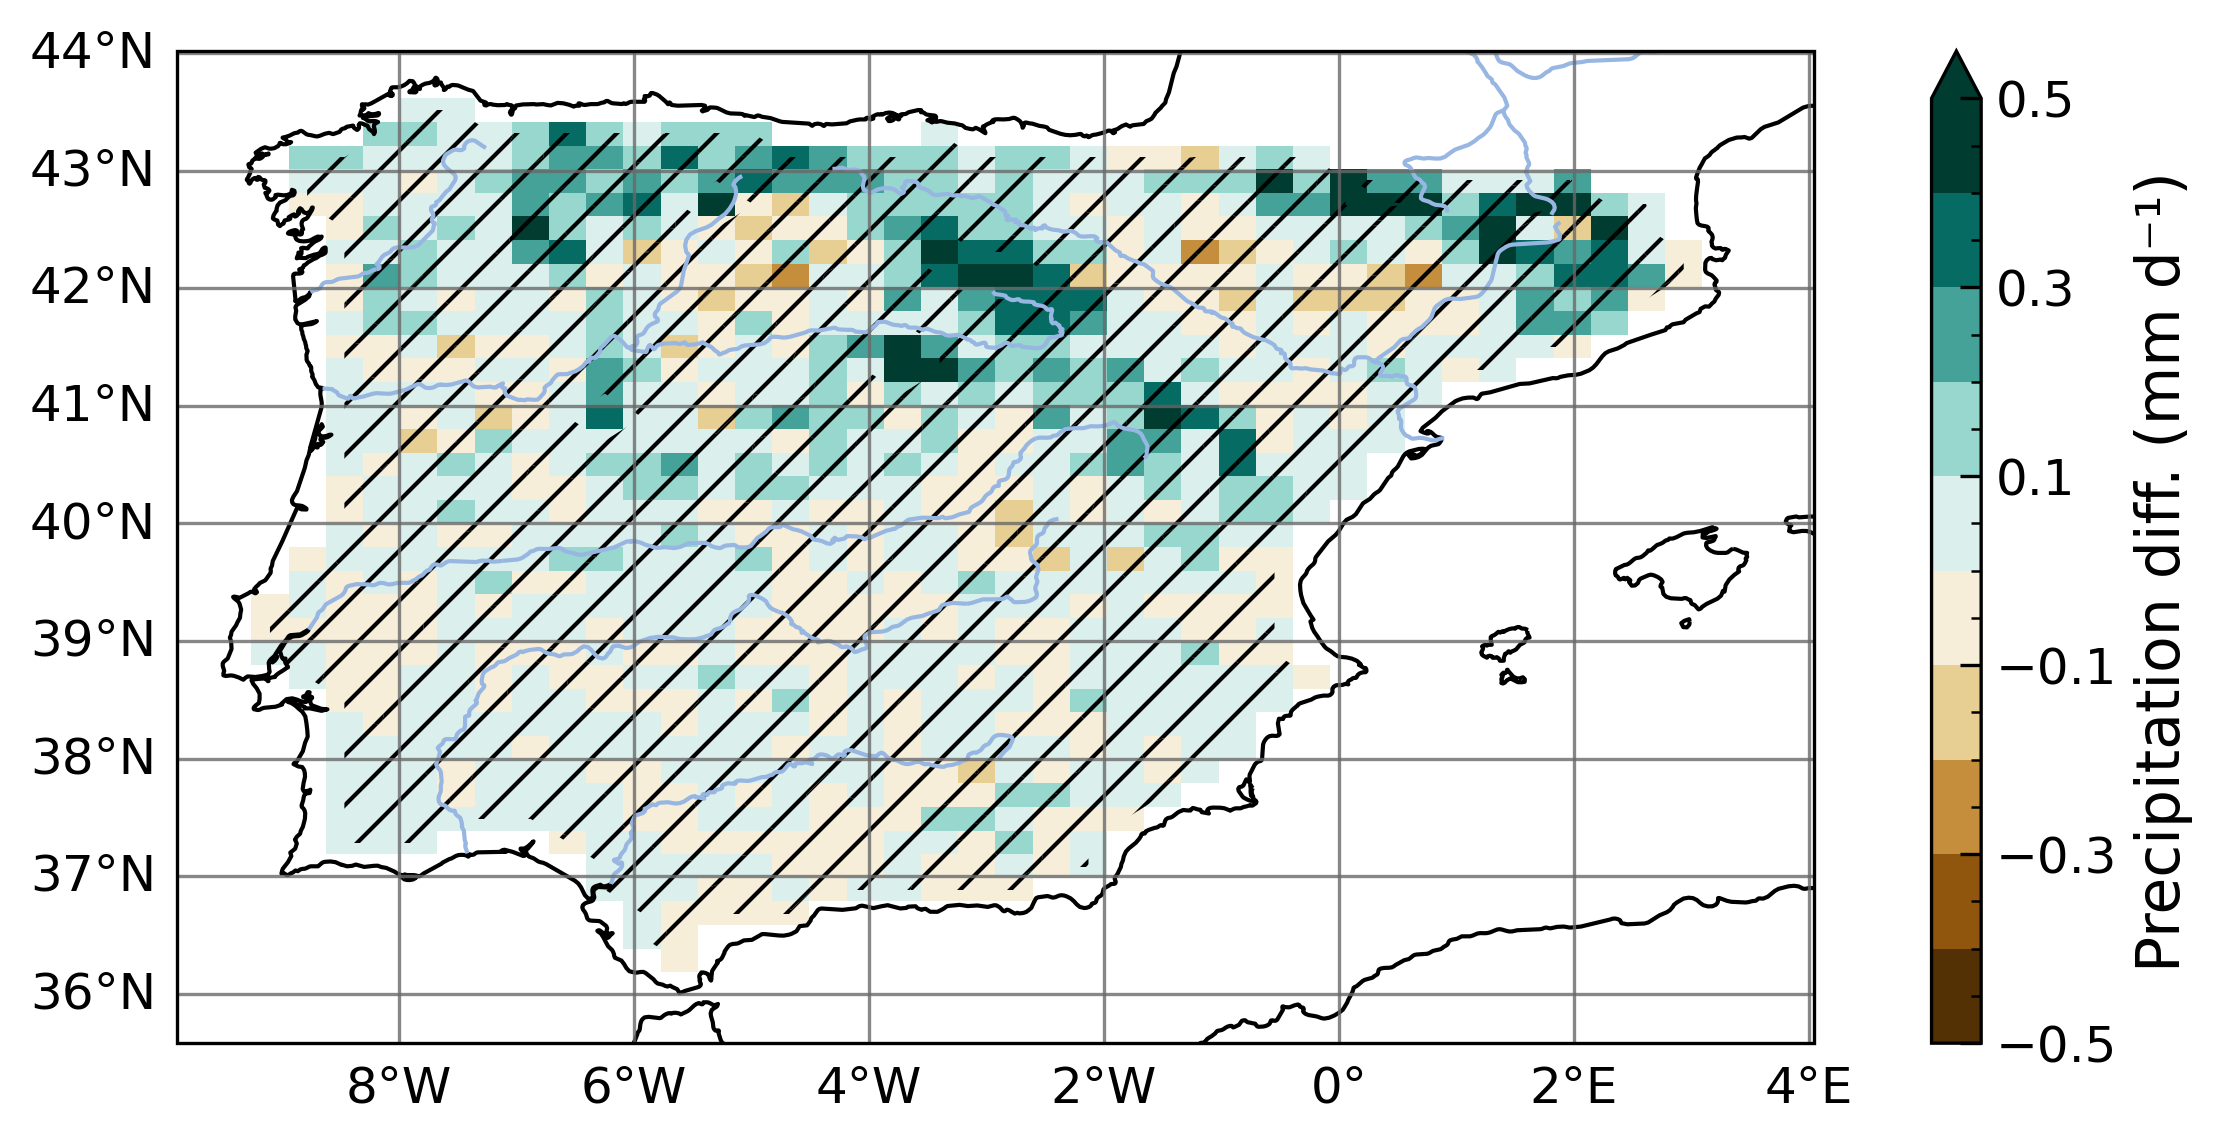
\includegraphics[width=\textwidth]{images/chap4/future/diffmap_JJA_precip_futirr.png}
%         \end{subfigure} &
%         %evap
%         \begin{subfigure}[b]{0.5\textwidth}
%             \caption{}
%             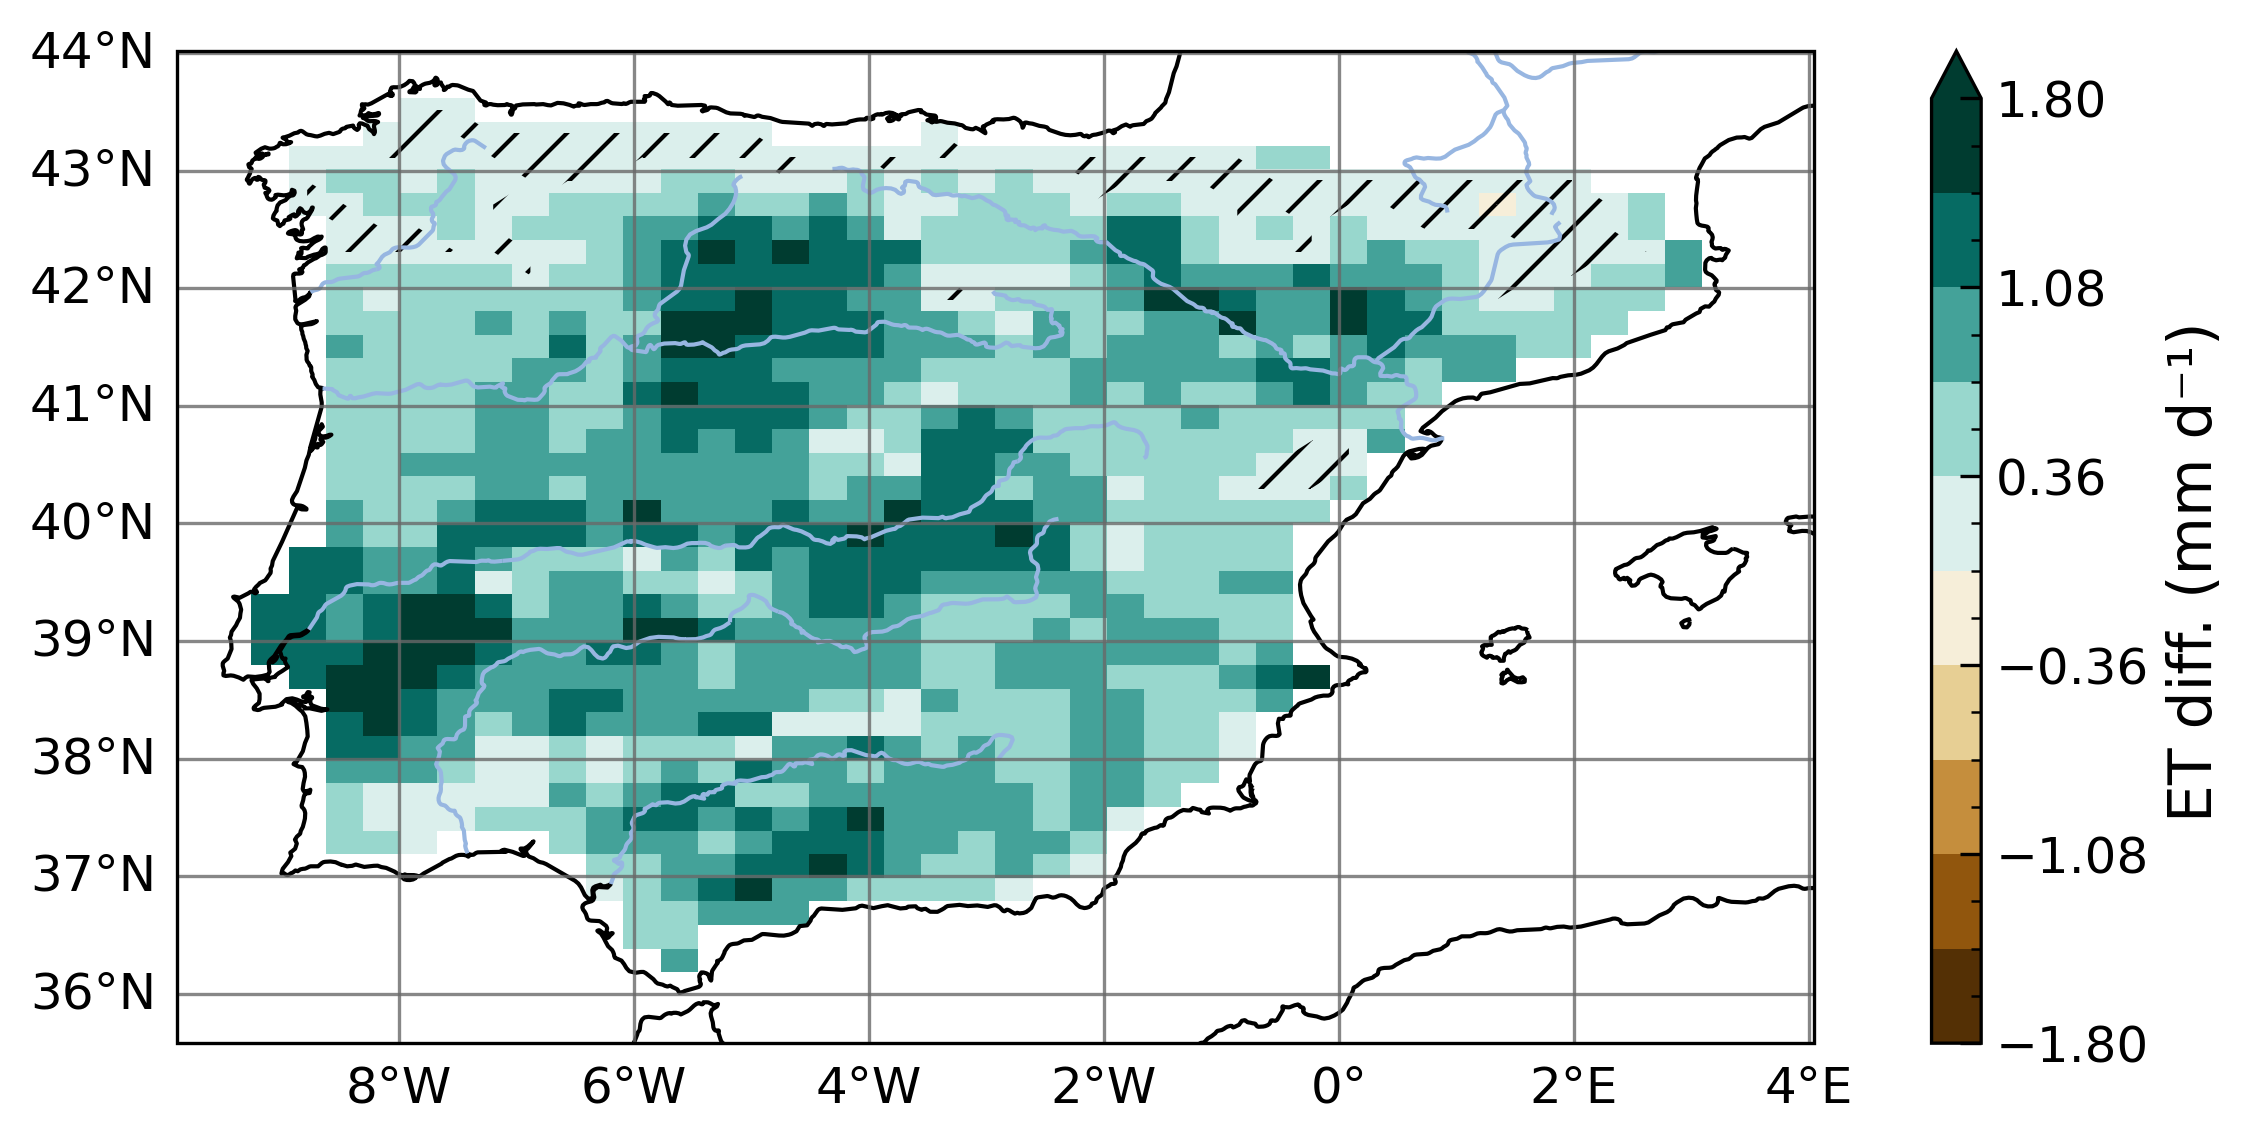
\includegraphics[width=\textwidth]{images/chap4/future/diffmap_JJA_evap_futirr.png}
%         \end{subfigure} \\

%         %t2m
%         \begin{subfigure}[b]{0.5\textwidth}
%             \caption{}
%             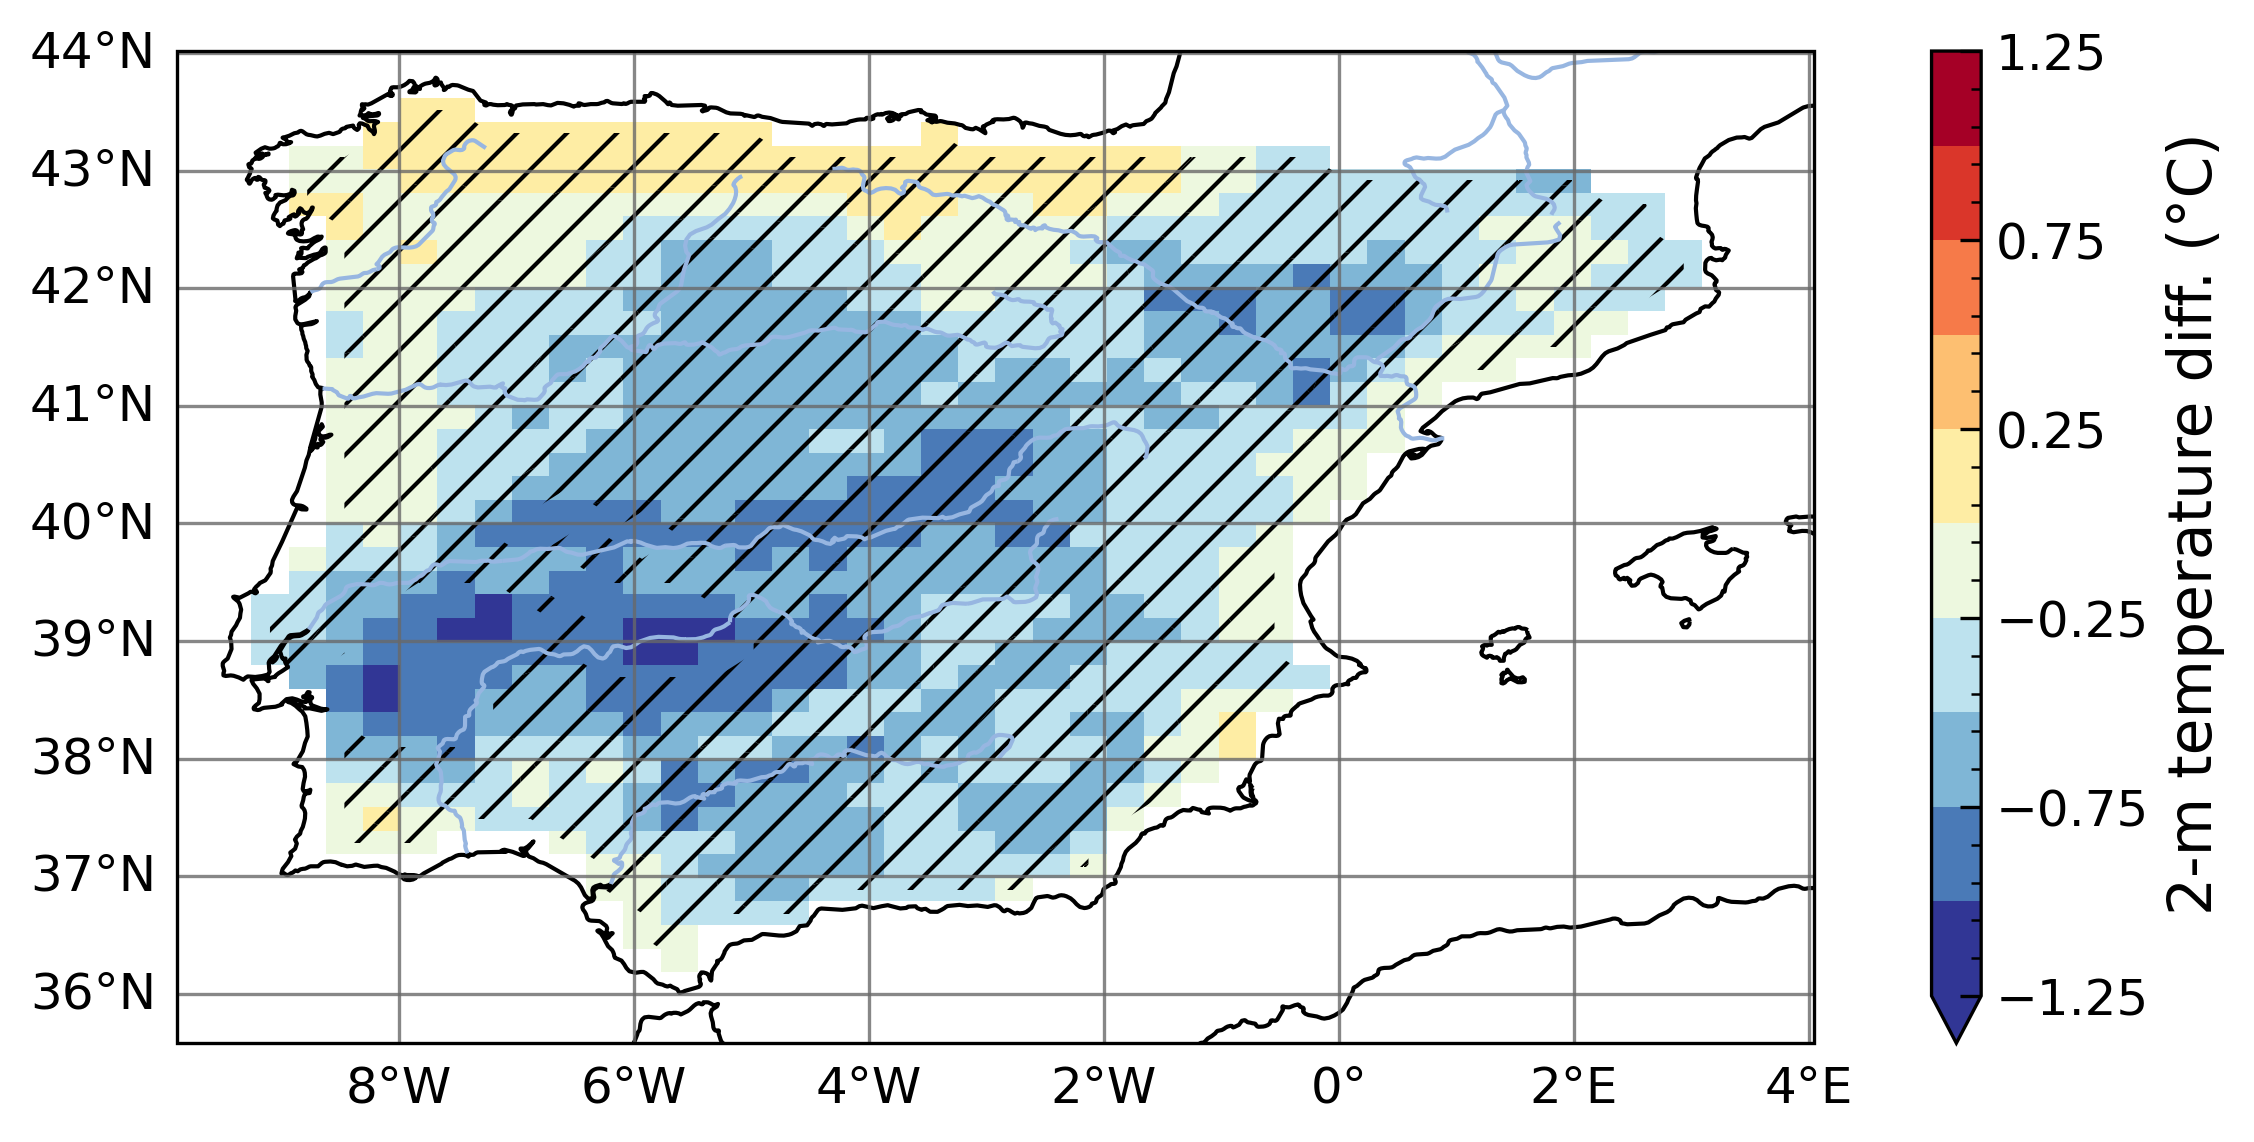
\includegraphics[width=\textwidth]{images/chap4/future/diffmap_JJA_t2m_futirr.png}
%         \end{subfigure} &
%         %fluxsens
%         \begin{subfigure}[b]{0.5\textwidth}
%             \caption{}
%             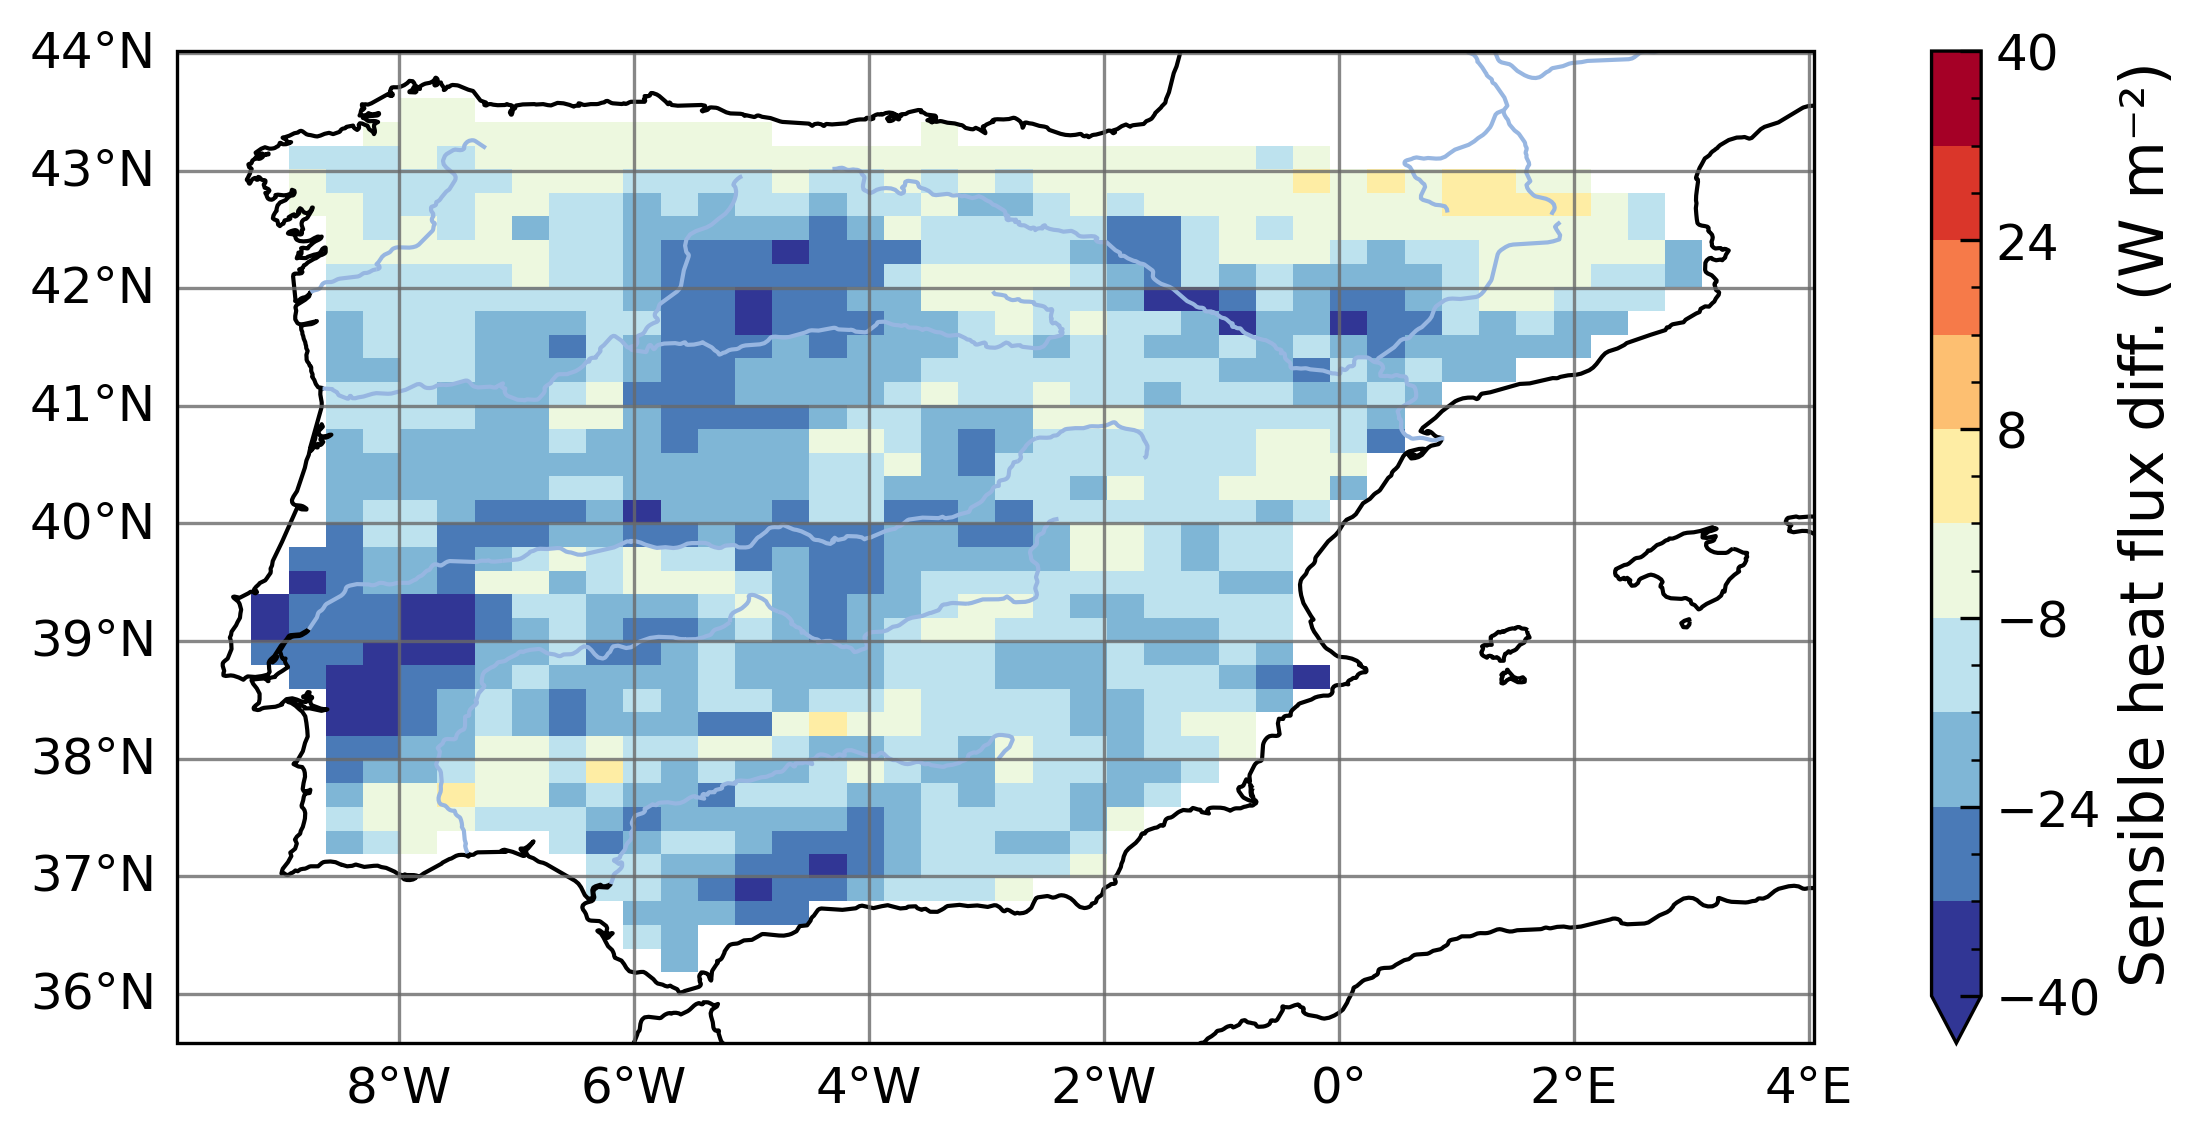
\includegraphics[width=\textwidth]{images/chap4/future/diffmap_JJA_fluxsens_futirr.png}
%         \end{subfigure} \\

%         %q2m
%         \begin{subfigure}[b]{0.5\textwidth}
%             \caption{}
%             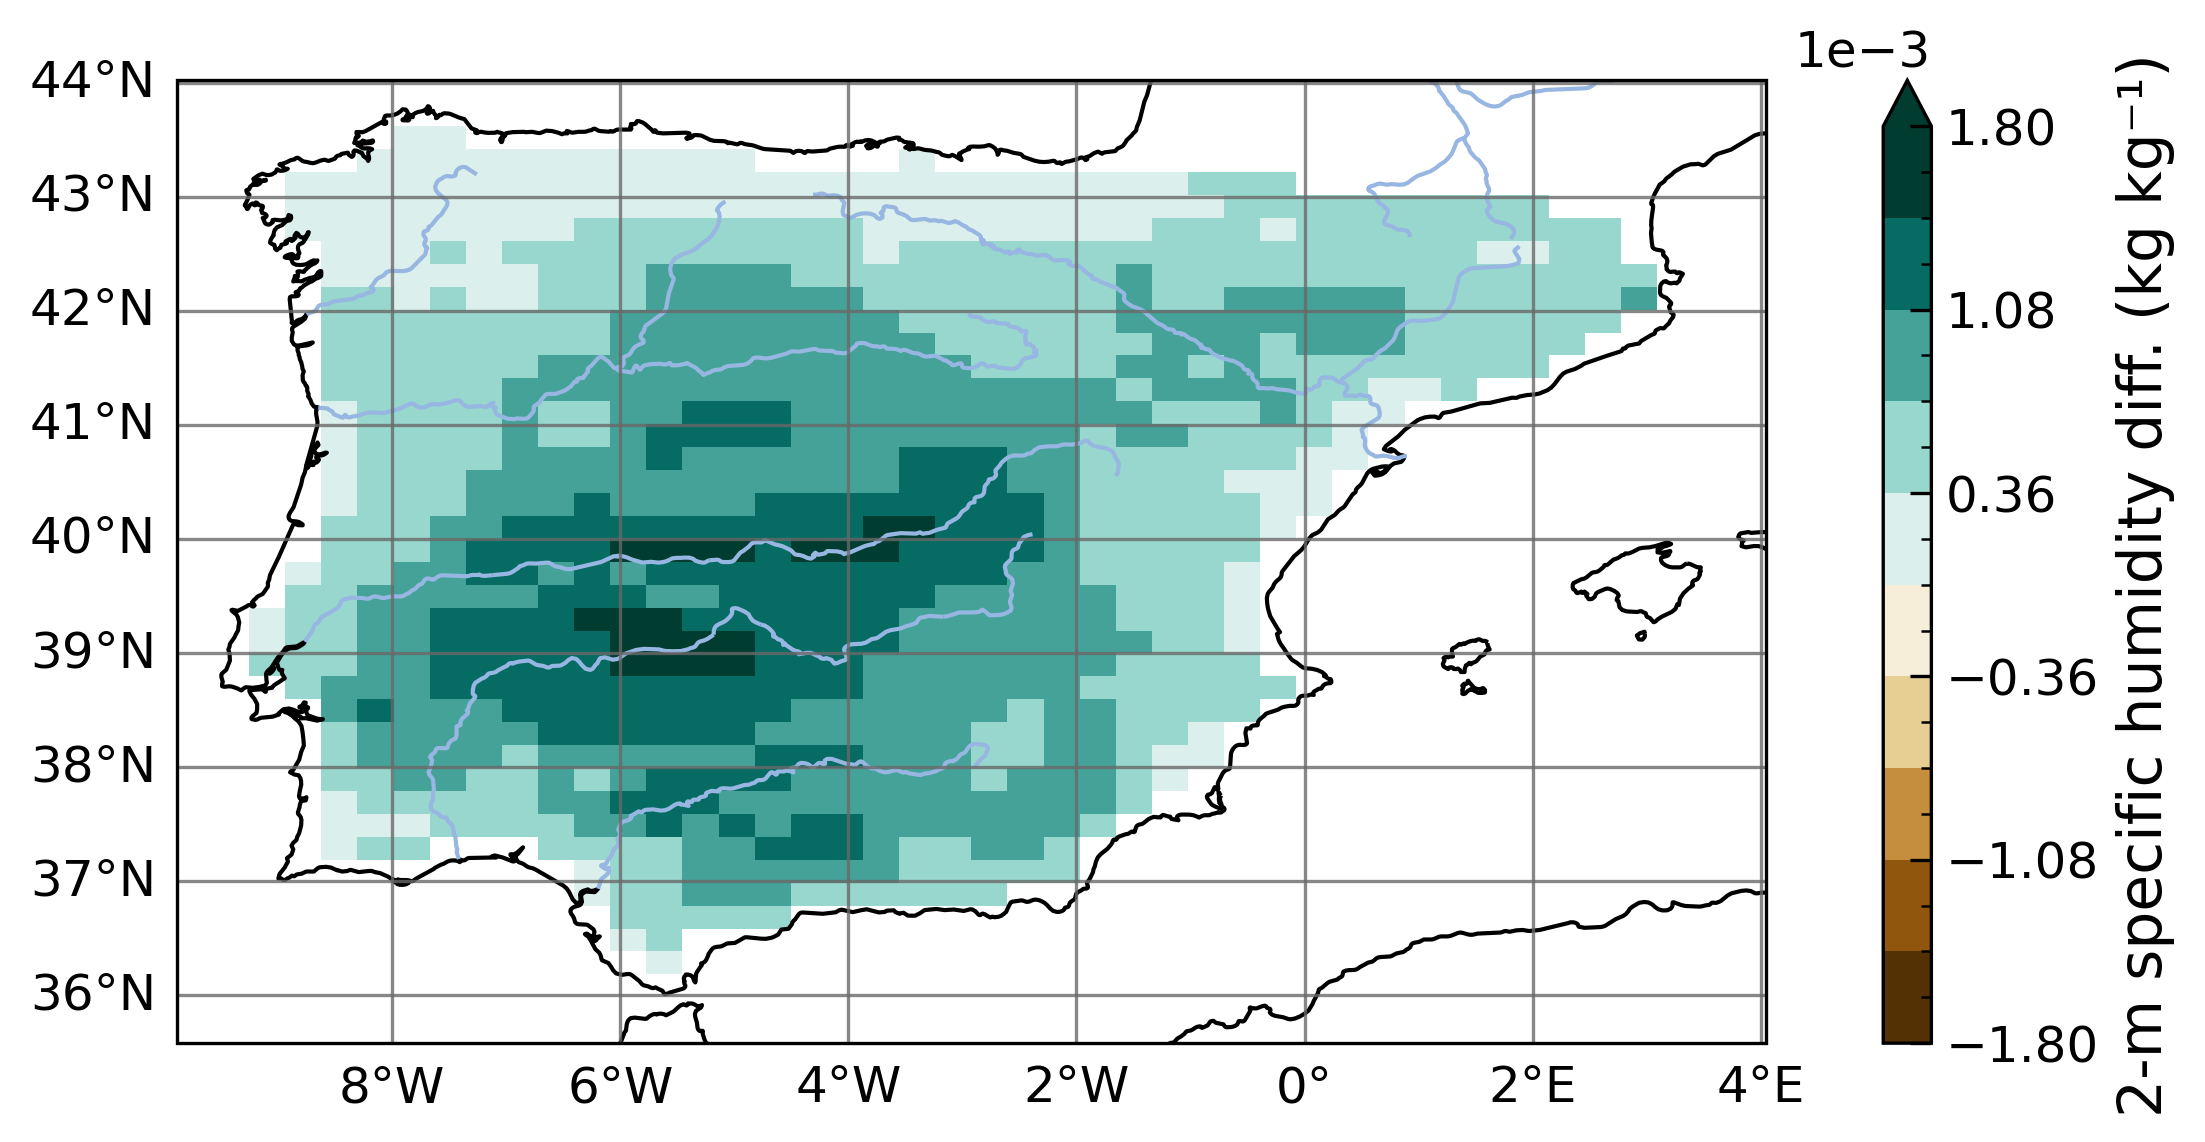
\includegraphics[width=\textwidth]{images/chap4/future/diffmap_JJA_q2m_futirr.png}
%         \end{subfigure} &
%         %rh2m
%         \begin{subfigure}[b]{0.5\textwidth}
%             \caption{}
%             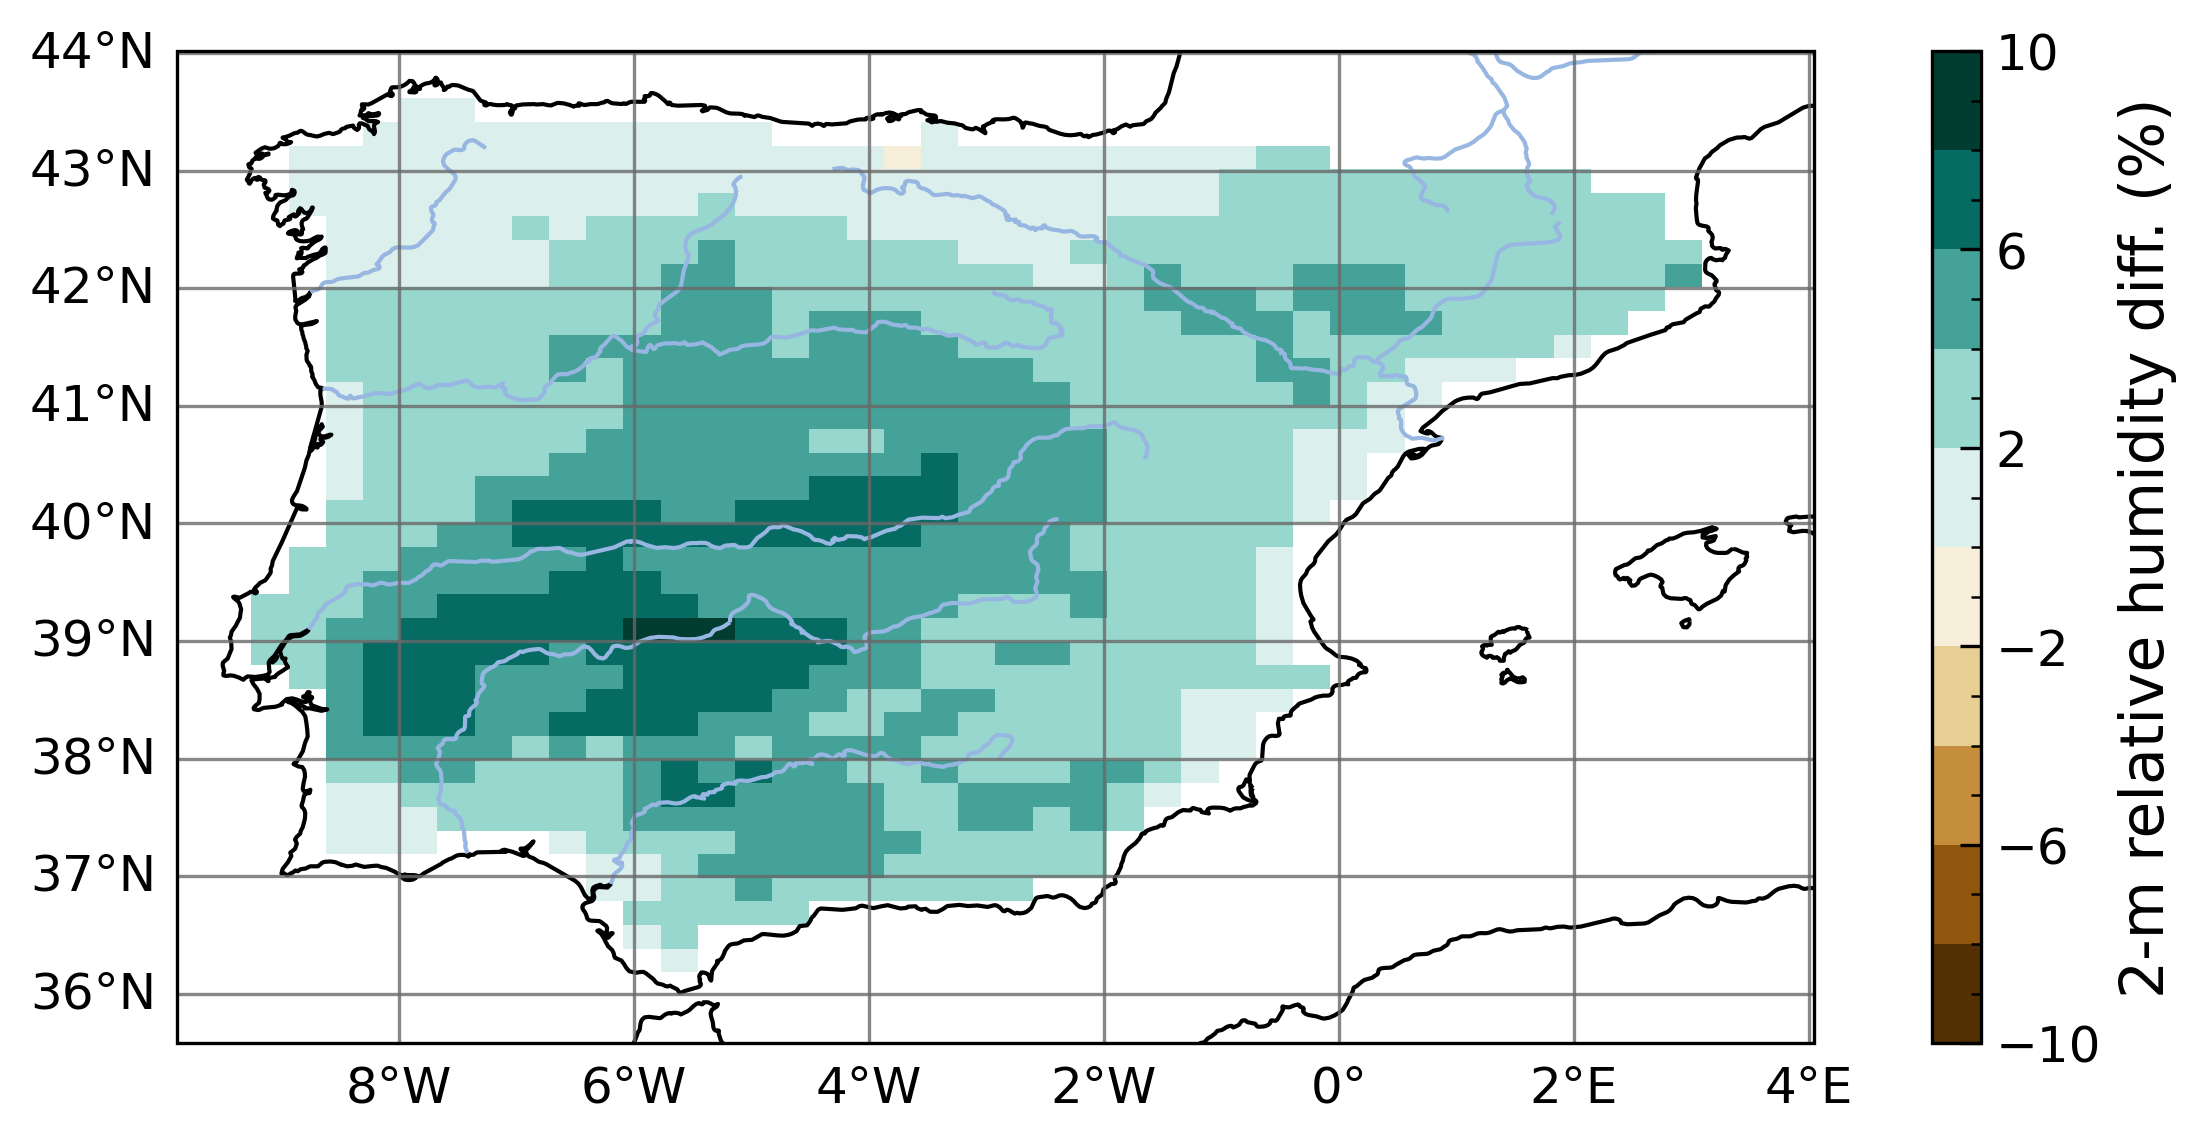
\includegraphics[width=\textwidth]{images/chap4/future/diffmap_JJA_rh2m_futirr.png}
%         \end{subfigure} \\

%         %pblh
%         \begin{subfigure}[b]{0.5\textwidth}
%             \caption{}
%             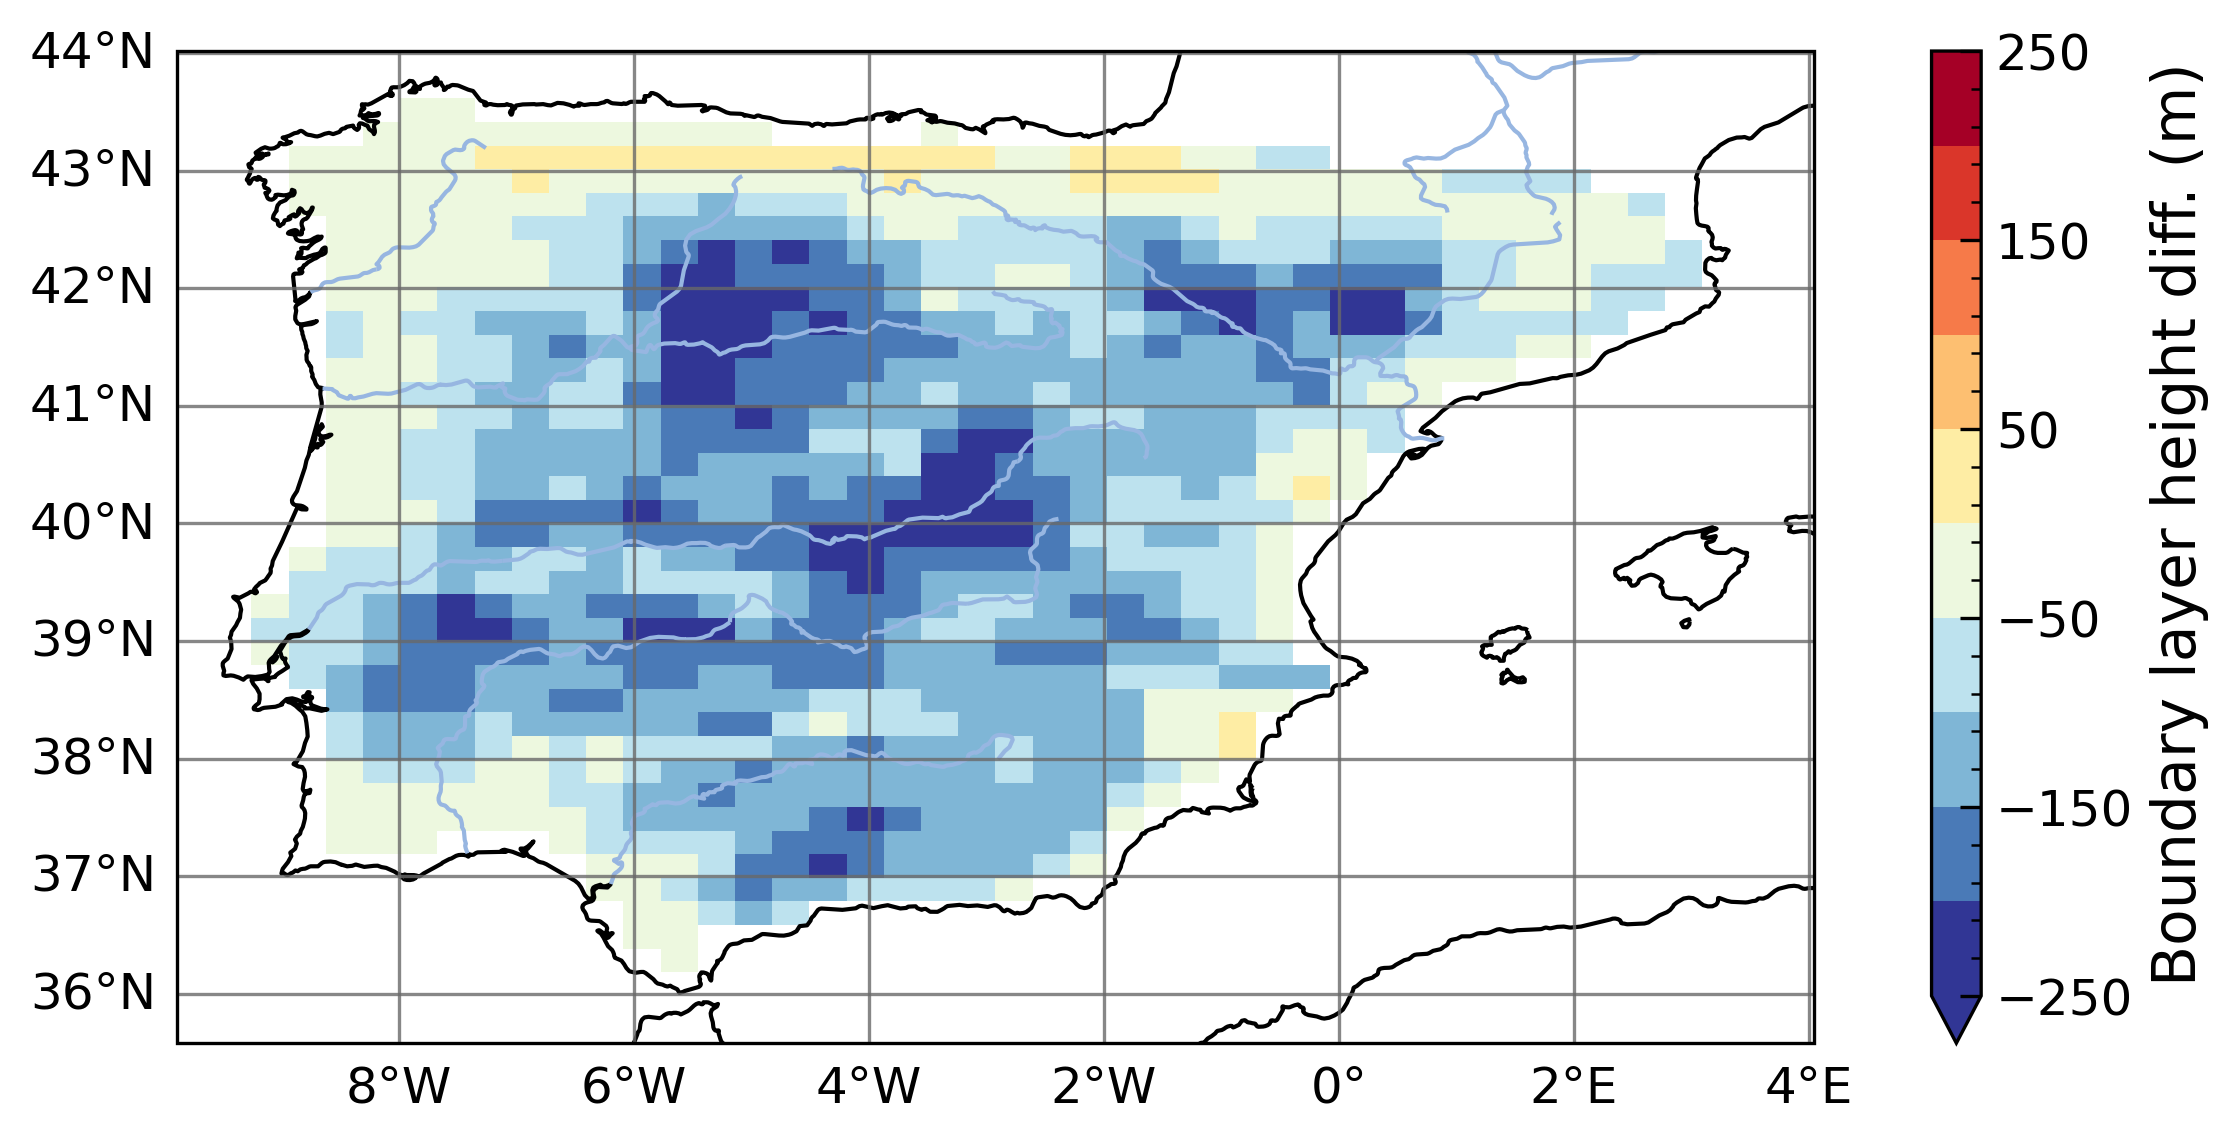
\includegraphics[width=\textwidth]{images/chap4/future/diffmap_JJA_s_pblh_futirr.png}
%         \end{subfigure} &
%         %lcl
%         \begin{subfigure}[b]{0.5\textwidth}
%             \caption{}
%             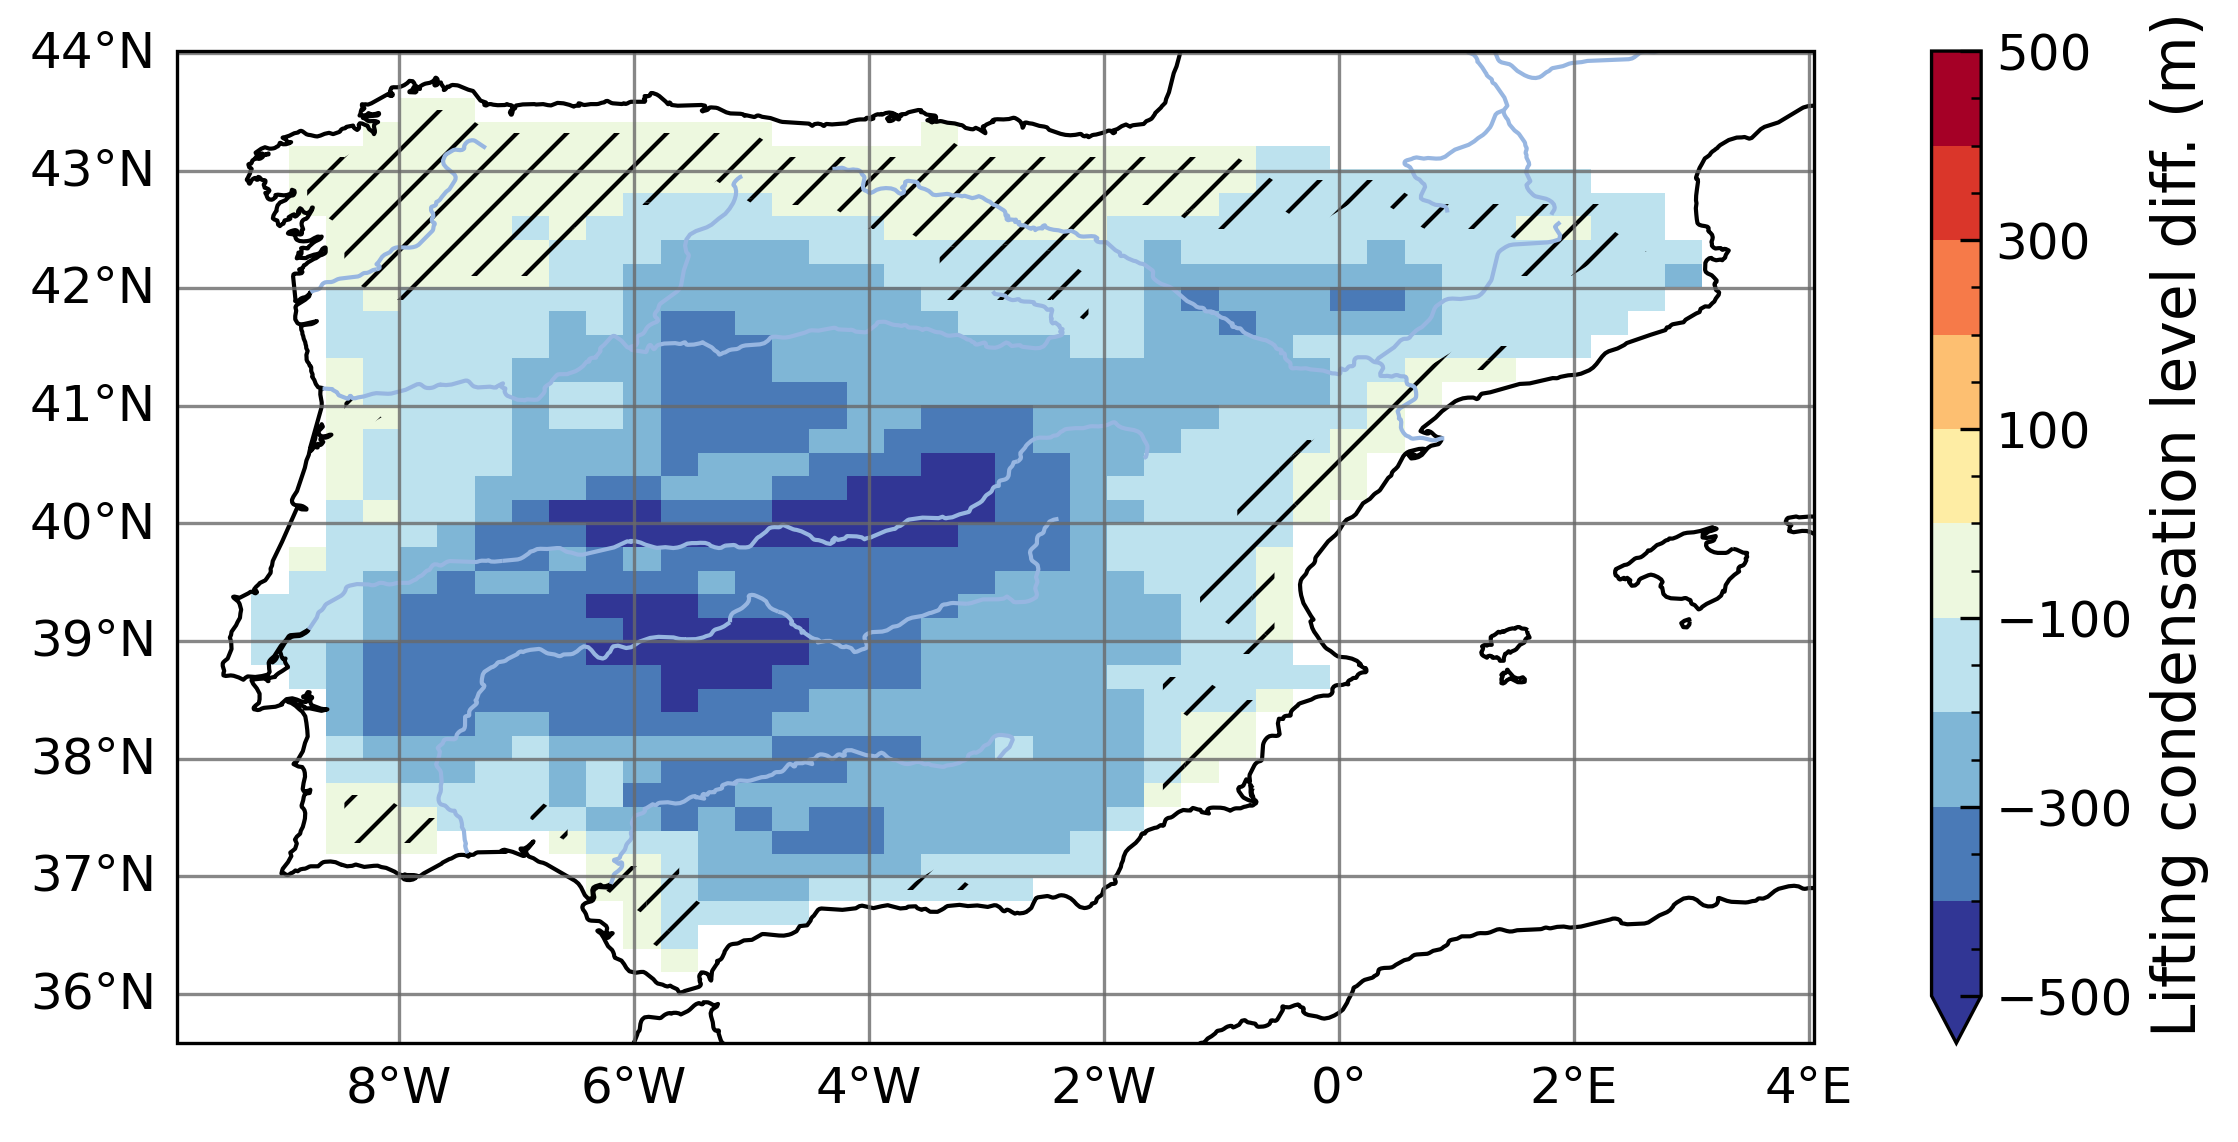
\includegraphics[width=\textwidth]{images/chap4/future/diffmap_JJA_s_lcl_futirr.png}
%         \end{subfigure} \\
%     \end{tabular}
%     \caption{JJA difference (\futnoirr - \futirr)}
%     \label{fig:diffmaps_JJA_future_irr}
% \end{figure}


%figure : rel diff maps (future, irr - no_irr)
\begin{figure}[htbp]
    \centering
    \begin{tabular}{cc}
        %precip
        \begin{subfigure}[b]{0.5\textwidth}
            \caption{}
            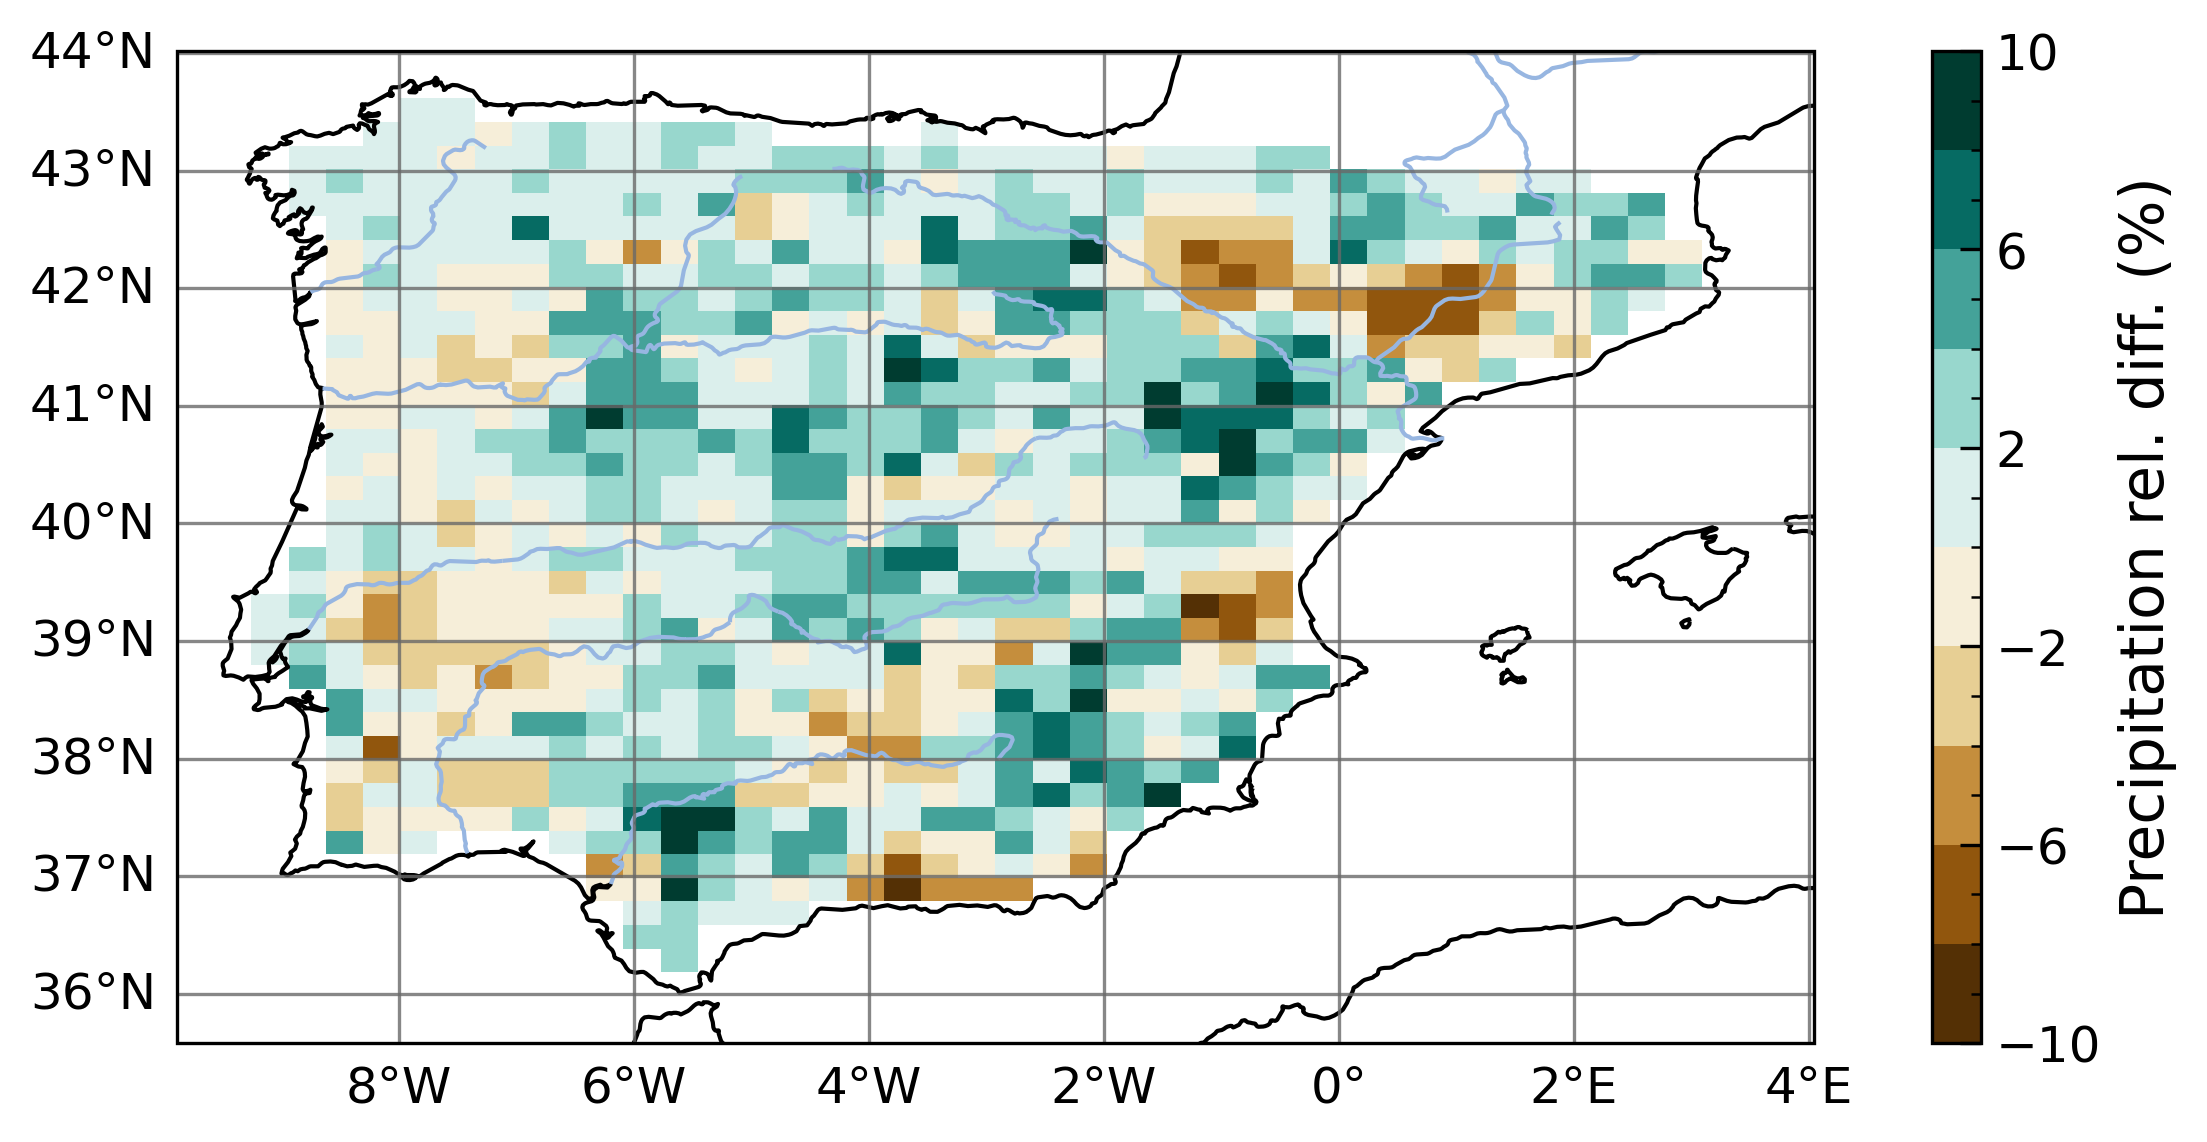
\includegraphics[width=\textwidth]{images/chap4/future/reldiffmap_precip_futirr.png}
        \end{subfigure} &
        %evap
        \begin{subfigure}[b]{0.5\textwidth}
            \caption{}
            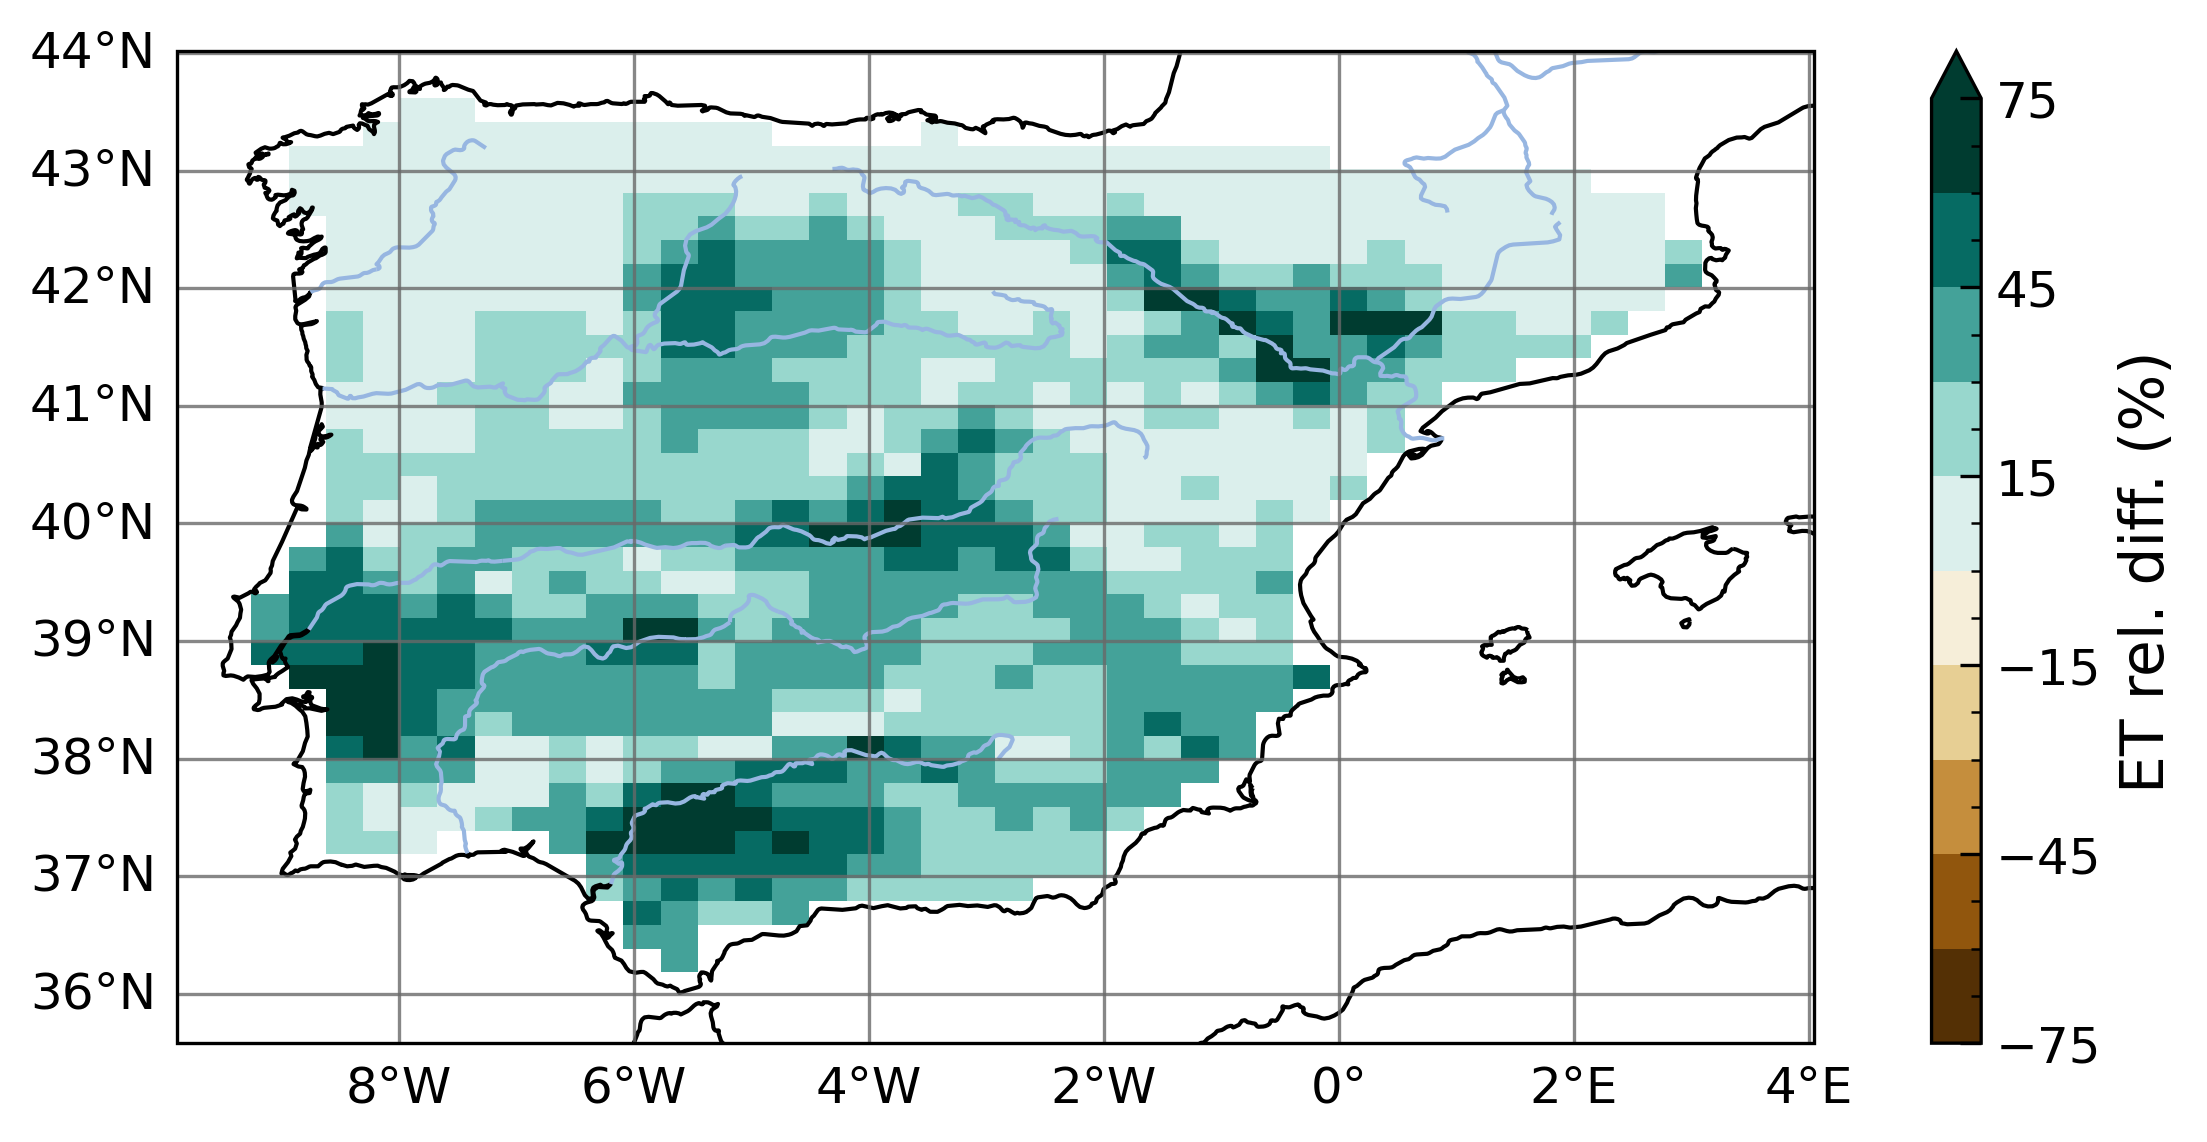
\includegraphics[width=\textwidth]{images/chap4/future/reldiffmap_evap_futirr.png}
        \end{subfigure} \\

        %t2m
        \begin{subfigure}[b]{0.5\textwidth}
            \caption{}
            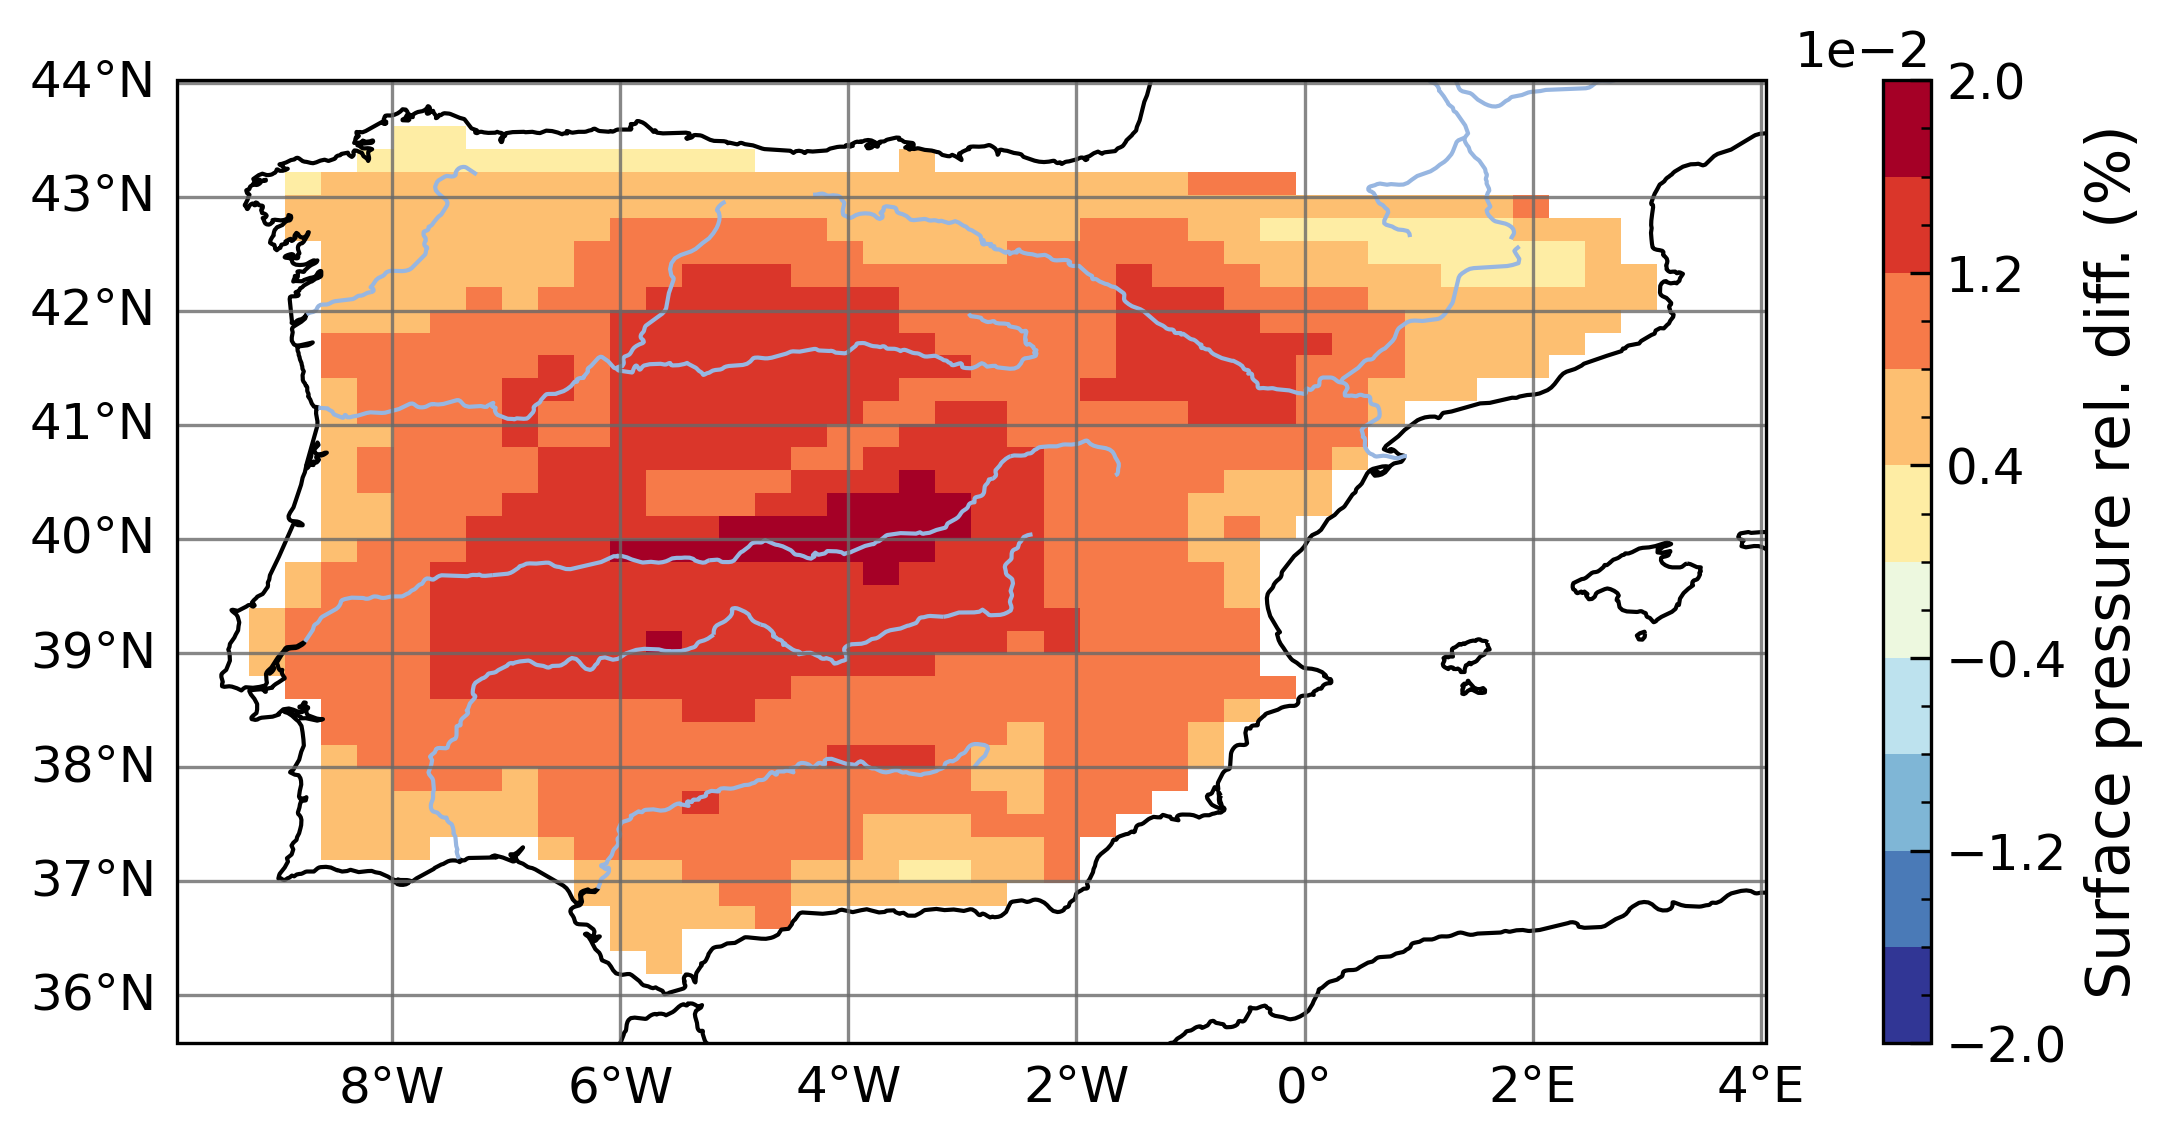
\includegraphics[width=\textwidth]{images/chap4/future/reldiffmap_psol_futirr.png}
        \end{subfigure} &
        %fluxsens
        \begin{subfigure}[b]{0.5\textwidth}
            \caption{}
            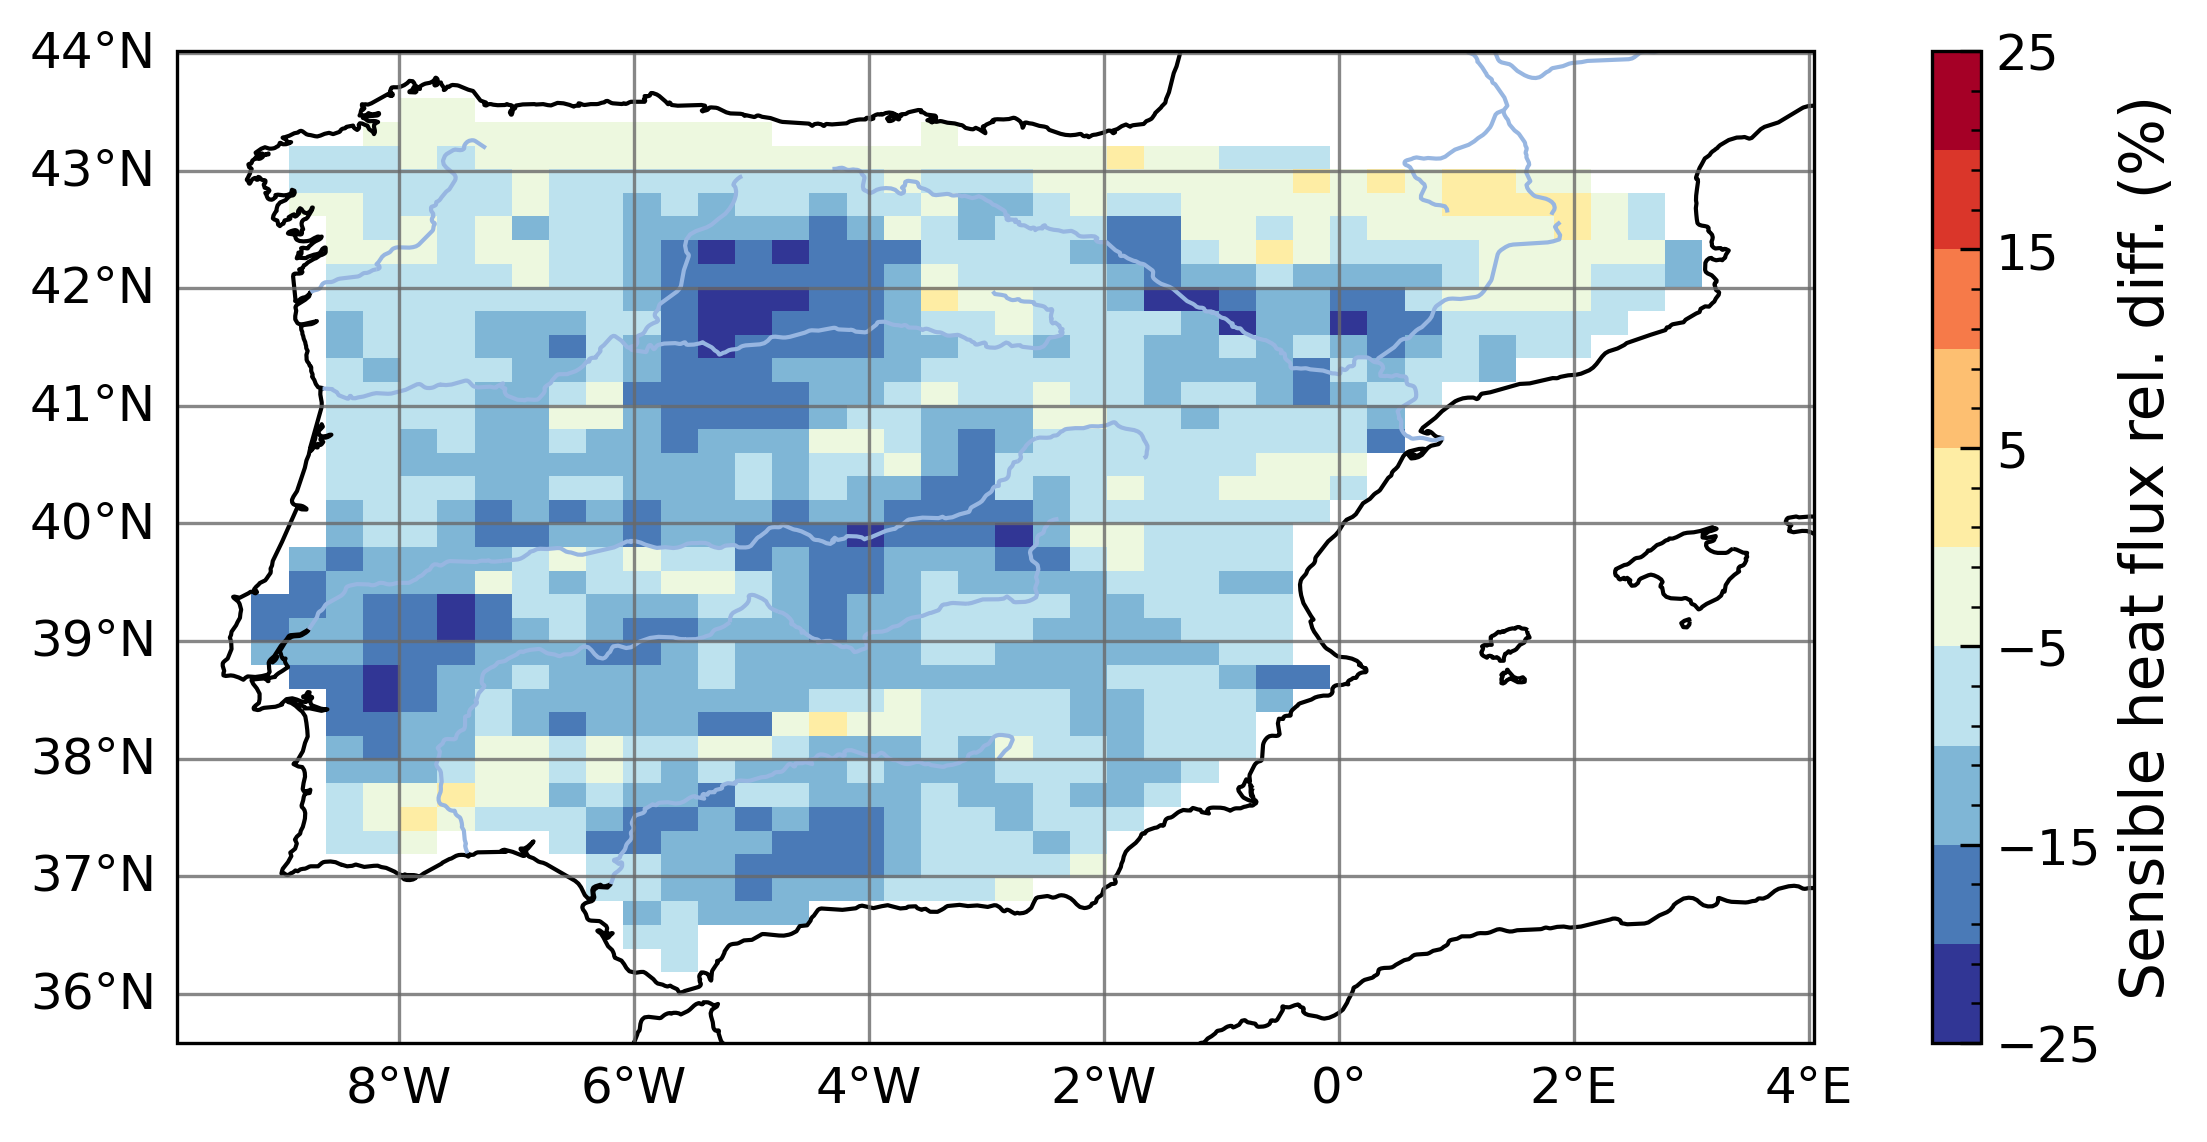
\includegraphics[width=\textwidth]{images/chap4/future/reldiffmap_fluxsens_futirr.png}
        \end{subfigure} \\

        %q2m
        \begin{subfigure}[b]{0.5\textwidth}
            \caption{}
            \includegraphics[width=\textwidth]{images/chap4/future/reldiffmap_q2m_futirr.png}
        \end{subfigure} &
        %rh2m
        \begin{subfigure}[b]{0.5\textwidth}
            \caption{}
            \includegraphics[width=\textwidth]{images/chap4/future/reldiffmap_rh2m_futirr.png}
        \end{subfigure} \\

        %pblh
        \begin{subfigure}[b]{0.5\textwidth}
            \caption{}
            \includegraphics[width=\textwidth]{images/chap4/future/reldiffmap_s_pblh_futirr.png}
        \end{subfigure} &
        %lcl
        \begin{subfigure}[b]{0.5\textwidth}
            \caption{}
            \includegraphics[width=\textwidth]{images/chap4/future/reldiffmap_s_lcl_futirr.png}
        \end{subfigure} \\
    \end{tabular}
    \caption{Annual relative difference (\futnoirr - \futirr)}
    \label{fig:reldiffmaps_future_irr}
\end{figure}

%figure : Aridity Index diff and rel diff maps
\begin{figure}[htbp]
    \centering
    \begin{tabular}{cc}
        %present vs future (noirr)
        \begin{subfigure}[b]{0.5\textwidth}
            \caption{Absolute change in aridity index under climate change}
            \includegraphics[width=\textwidth]{images/chap4/future/diffmap_aridity_index_presfut.png}
        \end{subfigure} &
        \begin{subfigure}[b]{0.5\textwidth}
            \caption{Relative change in aridity index under climate change}
            \includegraphics[width=\textwidth]{images/chap4/future/reldiffmap_aridity_index_presfut.png}
        \end{subfigure} \\

        %irr vs noirr (future)
        \begin{subfigure}[b]{0.5\textwidth}
            \caption{Absolute change in future aridity index in the presence of irrigation}
            \includegraphics[width=\textwidth]{images/chap4/future/diffmap_aridity_index_futirr.png}
        \end{subfigure} &
        \begin{subfigure}[b]{0.5\textwidth}
            \caption{Relative change in future aridity index in the presence of irrigation}
            \includegraphics[width=\textwidth]{images/chap4/future/reldiffmap_aridity_index_futirr.png}
        \end{subfigure} \\
    \end{tabular}
    \caption{Aridity index changes under climate change and in the presence of irrigation.}
    \label{fig:diffmaps_aridity}
\end{figure}

